% Options for packages loaded elsewhere
\PassOptionsToPackage{unicode}{hyperref}
\PassOptionsToPackage{hyphens}{url}
\PassOptionsToPackage{dvipsnames,svgnames*,x11names*}{xcolor}
%
\documentclass[
  11pt,
  american,
]{report}
\usepackage{amsmath,amssymb}
\usepackage{lmodern}
\usepackage{iftex}
\ifPDFTeX
  \usepackage[T1]{fontenc}
  \usepackage[utf8]{inputenc}
  \usepackage{textcomp} % provide euro and other symbols
\else % if luatex or xetex
  \usepackage{unicode-math}
  \defaultfontfeatures{Scale=MatchLowercase}
  \defaultfontfeatures[\rmfamily]{Ligatures=TeX,Scale=1}
  \setmainfont[]{Arial}
  \setsansfont[]{Arial}
  \setmonofont[]{Menlo}
\fi
% Use upquote if available, for straight quotes in verbatim environments
\IfFileExists{upquote.sty}{\usepackage{upquote}}{}
\IfFileExists{microtype.sty}{% use microtype if available
  \usepackage[]{microtype}
  \UseMicrotypeSet[protrusion]{basicmath} % disable protrusion for tt fonts
}{}
\makeatletter
\@ifundefined{KOMAClassName}{% if non-KOMA class
  \IfFileExists{parskip.sty}{%
    \usepackage{parskip}
  }{% else
    \setlength{\parindent}{0pt}
    \setlength{\parskip}{6pt plus 2pt minus 1pt}}
}{% if KOMA class
  \KOMAoptions{parskip=half}}
\makeatother
\usepackage{xcolor}
\IfFileExists{xurl.sty}{\usepackage{xurl}}{} % add URL line breaks if available
\IfFileExists{bookmark.sty}{\usepackage{bookmark}}{\usepackage{hyperref}}
\hypersetup{
  pdftitle={SolarLab Technical and User Manual},
  pdfauthor={SolarLab Project},
  pdflang={en-US},
  colorlinks=true,
  linkcolor={blue},
  filecolor={Maroon},
  citecolor={Blue},
  urlcolor={blue},
  pdfcreator={LaTeX via pandoc}}
\urlstyle{same} % disable monospaced font for URLs
\usepackage[margin=0.85in]{geometry}
\usepackage{color}
\usepackage{fancyvrb}
\newcommand{\VerbBar}{|}
\newcommand{\VERB}{\Verb[commandchars=\\\{\}]}
\DefineVerbatimEnvironment{Highlighting}{Verbatim}{commandchars=\\\{\}}
% Add ',fontsize=\small' for more characters per line
\newenvironment{Shaded}{}{}
\newcommand{\AlertTok}[1]{\textcolor[rgb]{1.00,0.00,0.00}{\textbf{#1}}}
\newcommand{\AnnotationTok}[1]{\textcolor[rgb]{0.38,0.63,0.69}{\textbf{\textit{#1}}}}
\newcommand{\AttributeTok}[1]{\textcolor[rgb]{0.49,0.56,0.16}{#1}}
\newcommand{\BaseNTok}[1]{\textcolor[rgb]{0.25,0.63,0.44}{#1}}
\newcommand{\BuiltInTok}[1]{#1}
\newcommand{\CharTok}[1]{\textcolor[rgb]{0.25,0.44,0.63}{#1}}
\newcommand{\CommentTok}[1]{\textcolor[rgb]{0.38,0.63,0.69}{\textit{#1}}}
\newcommand{\CommentVarTok}[1]{\textcolor[rgb]{0.38,0.63,0.69}{\textbf{\textit{#1}}}}
\newcommand{\ConstantTok}[1]{\textcolor[rgb]{0.53,0.00,0.00}{#1}}
\newcommand{\ControlFlowTok}[1]{\textcolor[rgb]{0.00,0.44,0.13}{\textbf{#1}}}
\newcommand{\DataTypeTok}[1]{\textcolor[rgb]{0.56,0.13,0.00}{#1}}
\newcommand{\DecValTok}[1]{\textcolor[rgb]{0.25,0.63,0.44}{#1}}
\newcommand{\DocumentationTok}[1]{\textcolor[rgb]{0.73,0.13,0.13}{\textit{#1}}}
\newcommand{\ErrorTok}[1]{\textcolor[rgb]{1.00,0.00,0.00}{\textbf{#1}}}
\newcommand{\ExtensionTok}[1]{#1}
\newcommand{\FloatTok}[1]{\textcolor[rgb]{0.25,0.63,0.44}{#1}}
\newcommand{\FunctionTok}[1]{\textcolor[rgb]{0.02,0.16,0.49}{#1}}
\newcommand{\ImportTok}[1]{#1}
\newcommand{\InformationTok}[1]{\textcolor[rgb]{0.38,0.63,0.69}{\textbf{\textit{#1}}}}
\newcommand{\KeywordTok}[1]{\textcolor[rgb]{0.00,0.44,0.13}{\textbf{#1}}}
\newcommand{\NormalTok}[1]{#1}
\newcommand{\OperatorTok}[1]{\textcolor[rgb]{0.40,0.40,0.40}{#1}}
\newcommand{\OtherTok}[1]{\textcolor[rgb]{0.00,0.44,0.13}{#1}}
\newcommand{\PreprocessorTok}[1]{\textcolor[rgb]{0.74,0.48,0.00}{#1}}
\newcommand{\RegionMarkerTok}[1]{#1}
\newcommand{\SpecialCharTok}[1]{\textcolor[rgb]{0.25,0.44,0.63}{#1}}
\newcommand{\SpecialStringTok}[1]{\textcolor[rgb]{0.73,0.40,0.53}{#1}}
\newcommand{\StringTok}[1]{\textcolor[rgb]{0.25,0.44,0.63}{#1}}
\newcommand{\VariableTok}[1]{\textcolor[rgb]{0.10,0.09,0.49}{#1}}
\newcommand{\VerbatimStringTok}[1]{\textcolor[rgb]{0.25,0.44,0.63}{#1}}
\newcommand{\WarningTok}[1]{\textcolor[rgb]{0.38,0.63,0.69}{\textbf{\textit{#1}}}}
\usepackage{longtable,booktabs,array}
\usepackage{calc} % for calculating minipage widths
% Correct order of tables after \paragraph or \subparagraph
\usepackage{etoolbox}
\makeatletter
\patchcmd\longtable{\par}{\if@noskipsec\mbox{}\fi\par}{}{}
\makeatother
% Allow footnotes in longtable head/foot
\IfFileExists{footnotehyper.sty}{\usepackage{footnotehyper}}{\usepackage{footnote}}
\makesavenoteenv{longtable}
\usepackage{graphicx}
\makeatletter
\def\maxwidth{\ifdim\Gin@nat@width>\linewidth\linewidth\else\Gin@nat@width\fi}
\def\maxheight{\ifdim\Gin@nat@height>\textheight\textheight\else\Gin@nat@height\fi}
\makeatother
% Scale images if necessary, so that they will not overflow the page
% margins by default, and it is still possible to overwrite the defaults
% using explicit options in \includegraphics[width, height, ...]{}
\setkeys{Gin}{width=\maxwidth,height=\maxheight,keepaspectratio}
% Set default figure placement to htbp
\makeatletter
\def\fps@figure{htbp}
\makeatother
\setlength{\emergencystretch}{3em} % prevent overfull lines
\providecommand{\tightlist}{%
  \setlength{\itemsep}{0pt}\setlength{\parskip}{0pt}}
\setcounter{secnumdepth}{5}
\hypersetup{linktoc=all}
\usepackage{float}
\floatplacement{figure}{H}
\setlength{\abovecaptionskip}{4pt}
\setlength{\belowcaptionskip}{0pt}
\setlength{\intextsep}{7pt plus 2pt minus 2pt}
\setlength{\textfloatsep}{8pt plus 2pt minus 2pt}
\widowpenalty=10000
\clubpenalty=10000
\displaywidowpenalty=10000
\makeatletter
\renewcommand*\l@section{\@dottedtocline{1}{1.5em}{3.2em}}
\renewcommand*\l@subsection{\@dottedtocline{2}{4.7em}{4.1em}}
\makeatother
\ifXeTeX
  % Load polyglossia as late as possible: uses bidi with RTL langages (e.g. Hebrew, Arabic)
  \usepackage{polyglossia}
  \setmainlanguage[variant=american]{english}
\else
  \usepackage[main=american]{babel}
% get rid of language-specific shorthands (see #6817):
\let\LanguageShortHands\languageshorthands
\def\languageshorthands#1{}
\fi
\ifLuaTeX
  \usepackage{selnolig}  % disable illegal ligatures
\fi

\title{SolarLab Technical and User Manual}
\usepackage{etoolbox}
\makeatletter
\providecommand{\subtitle}[1]{% add subtitle to \maketitle
  \apptocmd{\@title}{\par {\large #1 \par}}{}{}
}
\makeatother
\subtitle{Technical guide to thin-film solar-cell simulation, workflows,
and validation}
\author{SolarLab Project}
\date{2026-08-11}

\begin{document}
\maketitle

{
\hypersetup{linkcolor=}
\setcounter{tocdepth}{2}
\tableofcontents
}
\listoffigures
\newpage

\hypertarget{executive-summary}{%
\chapter{Executive Summary}\label{executive-summary}}

SolarLab is a thin-film photovoltaic device simulator that couples
drift-diffusion transport, Poisson electrostatics, mobile-ion
redistribution, recombination, and optical generation within a
reproducible software workflow. The numerical core is exposed through a
Python API, a FastAPI service layer, and a TypeScript/Plotly
workstation. An experimental two-dimensional extension supports lateral
microstructure and grain-boundary studies.

This edition covers the cancellation-safe quasi-Fermi steady-state
solver, its small-signal frequency-domain extension, and the optional
zero-thickness heterointerface model. At that interface, the quasi-Fermi
solver removes the ordinary Scharfetter-Gummel face and solves
thermionic transport and interface-SRH recombination together.
Unsupported physics produces an error before Newton starts. The
transient and direct steady-state solvers are still available for the
device classes they support.

New device files also state how the contact voltage is obtained.
SolarLab can calculate the signed built-in potential from the two
semiconductor contact work functions or from two specified metal work
functions. Carrier exchange at the contacts is configured separately. A
manual \texttt{V\_bi} is reserved for legacy benchmarks in which that
value forms part of the published comparison.

This manual serves two purposes:

\begin{enumerate}
\def\labelenumi{\arabic{enumi}.}
\tightlist
\item
  It introduces the device variables, parameter conventions, and
  simulation workflow for readers who are new to SolarLab or to
  semiconductor device simulation.
\item
  It documents the implemented physics, numerical method, validation
  gates, assumptions, and limitations needed for technical review and
  reproducible use.
\end{enumerate}

Chapter \ref{validation-and-evidence} lists the test runs, benchmark
ranges and source state used for this edition. The following chapter
collects the model assumptions and known limits.

\hypertarget{how-to-read-this-manual}{%
\chapter{How To Read This Manual}\label{how-to-read-this-manual}}

If you are new to device simulation, read the chapters in order through
\emph{Device Definition}, \emph{Governing Equations}, and
\emph{Numerical Method}. These chapters explain the device, the
variables, the equations, and the numerical method before introducing
the software workflow.

If you are already familiar with semiconductor drift-diffusion, start
with:

\begin{itemize}
\tightlist
\item
  Chapter \ref{governing-equations} (\emph{Governing Equations}), which
  defines the physical model in continuous form;
\item
  Chapter \ref{numerical-method} (\emph{Numerical Method}), which
  describes the discretization, the time integrator, and the
  steady-state solver;
\item
  Chapter \ref{running-solarlab} (\emph{Running SolarLab}), which covers
  the YAML/Python/API workflows;
\item
  Chapter \ref{validation-and-evidence} (\emph{Validation And
  Evidence}), which gives validation evidence and limitations.
\end{itemize}

The notation in this manual follows standard solar-cell convention:

\begin{itemize}
\tightlist
\item
  \(V_\mathrm{oc}\): open-circuit voltage.
\item
  \(J_\mathrm{sc}\): short-circuit current density.
\item
  \(FF\): fill factor.
\item
  \(PCE\): power-conversion efficiency.
\item
  \(n\): electron density.
\item
  \(p\): hole density.
\item
  \(P\): mobile positive ion-vacancy density.
\item
  \(\phi\): electrostatic potential.
\item
  \(E\): electric field.
\item
  \(G\): optical generation rate.
\item
  \(R\): recombination rate.
\end{itemize}

All simulator inputs are SI unless explicitly stated otherwise. Length
is in meters, time in seconds, current density in \(A\,m^{-2}\), density
in \(m^{-3}\), mobility in \(m^2 V^{-1} s^{-1}\), and diffusion
coefficient in \(m^2 s^{-1}\). The electron affinity \(\chi\) and band
gap \(E_g\) are stored in eV.

\hypertarget{simulator-architecture}{%
\chapter{Simulator Architecture}\label{simulator-architecture}}

SolarLab uses one device schema throughout the program. YAML files, the
Python API, the FastAPI backend and the TypeScript frontend all create
the same \texttt{DeviceStack} object, so a value edited in the browser
reaches the same solver input as a value loaded from YAML.

\begin{figure}
\centering
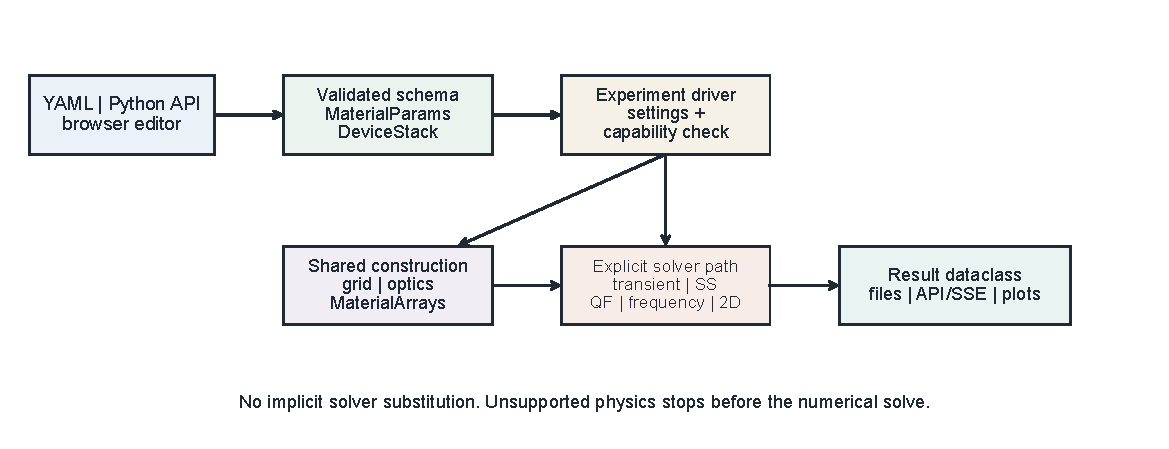
\includegraphics[width=0.98\textwidth,height=\textheight]{figures/architecture_flow.pdf}
\caption{SolarLab architecture and data flow}
\end{figure}

Four implementation rules keep these layers consistent:

\begin{itemize}
\tightlist
\item
  device definition is separated from experiment settings;
\item
  material and grid arrays are cached before the time integrator runs;
\item
  physics hooks are activated by the resolved simulation mode and by the
  presence of required parameters;
\item
  backend and frontend layers transport result dataclasses instead of
  reimplementing solver logic.
\end{itemize}

The experiment selects its solver explicitly. \texttt{transient},
\texttt{steady\_state} and \texttt{quasi\_fermi} use different state
variables and support different physics. SolarLab never swaps one for
another automatically; an unsupported combination stops before the
solve.

\hypertarget{solver-and-model-scope}{%
\section{Solver And Model Scope}\label{solver-and-model-scope}}

No single driver includes every optional model. The physics tier chooses
which configured terms may run, while the experiment driver sets the
unknowns, boundary conditions and numerical checks. Record both with the
result.

\begingroup\footnotesize\setlength{\tabcolsep}{3.5pt}\renewcommand{\arraystretch}{1.18}
\begin{longtable}{@{}>{\raggedright\arraybackslash}p{0.15\linewidth}>{\raggedright\arraybackslash}p{0.20\linewidth}>{\raggedright\arraybackslash}p{0.29\linewidth}>{\raggedright\arraybackslash}p{0.28\linewidth}@{}}
\toprule
Driver & Intended quantity & Physical model & Main limitation \\
\midrule
\endhead
\path{transient} & state-preserving J-V, hysteresis and time response & density variables; coupled electrons, holes and configured mobile ions; full-tier Robin contacts, field mobility and non-local recycling where configured & the final state depends on the voltage/time history and settling protocol \\
\path{steady_state} & ion-frozen DC comparison & direct density-log Newton on the established 1D RHS; the seed ion profile is held fixed & ions do not relax; deep-CBO points may need the validated transient fallback \\
\path{quasi_fermi} & cancellation-safe local DC J-V & quasi-Fermi increments, eliminated Poisson response and separate continuity/current checks; optional zero-thickness interface model & limited to ion-free local physics with ideal carrier pins; unsupported hooks stop before Newton \\
\path{quasi_fermi_frequency} & restricted small-signal C-V/impedance & linear response about a certified local QF operating point & limited to the local model supported by the QF operating point \\
1D operator split & long-time ion/degradation evolution & ions advance with carriers frozen, followed by electronic re-equilibration & first-order split; check macro-step halving against the coupled transient \\
2D & lateral parity and microstructure & 2D electrostatics and carrier transport with the configured static ion background & ions remain fixed during the 2D J-V solve; validation covers the registered parity and microstructure cases \\
\bottomrule
\end{longtable}
\endgroup

\texttt{full} is a feature setting, not an accuracy grade. It enables
the widest set of hooks available to the selected driver, but support
and validation still depend on the device and experiment. For each
reported curve, record the device stack, physics tier, experiment driver
and solver settings.

\hypertarget{what-solarlab-simulates}{%
\chapter{What SolarLab Simulates}\label{what-solarlab-simulates}}

SolarLab represents a solar cell as a sequence of material layers
between two contacts. The default coordinate follows the stack
direction. Incident light generates electron-hole pairs, while the
electrostatic field and contact selectivity drive carrier separation and
extraction. In perovskite devices, mobile ionic defects can redistribute
under the same field, producing history-dependent current-voltage
response.

The default solver is one-dimensional and is appropriate for:

\begin{itemize}
\tightlist
\item
  J-V sweeps and hysteresis;
\item
  dark diode curves;
\item
  EQE and electroluminescence;
\item
  impedance;
\item
  residual-certified local QF J-V and frequency-domain C-V for supported
  ion-free stacks;
\item
  opt-in abrupt-interface transport/recombination studies with a
  zero-thickness physical boundary;
\item
  transient photovoltage;
\item
  ion-coupled degradation;
\item
  tandem current matching;
\item
  screening many material candidates.
\end{itemize}

SolarLab also includes an experimental two-dimensional solver. The 2D
solver extrudes the same vertical device stack laterally and is intended
for:

\begin{itemize}
\tightlist
\item
  1D/2D parity checks;
\item
  vertical grain boundaries;
\item
  lateral microstructure;
\item
  \(V_\mathrm{oc}(L_g)\) grain-size sweeps.
\end{itemize}

The 2D solver is not a replacement for the 1D workflow. Mobile ions are
held as a static Poisson background during 2D J-V runs; this is an
explicit model assumption and should be reported when interpreting 2D
results.

\begin{figure}
\centering
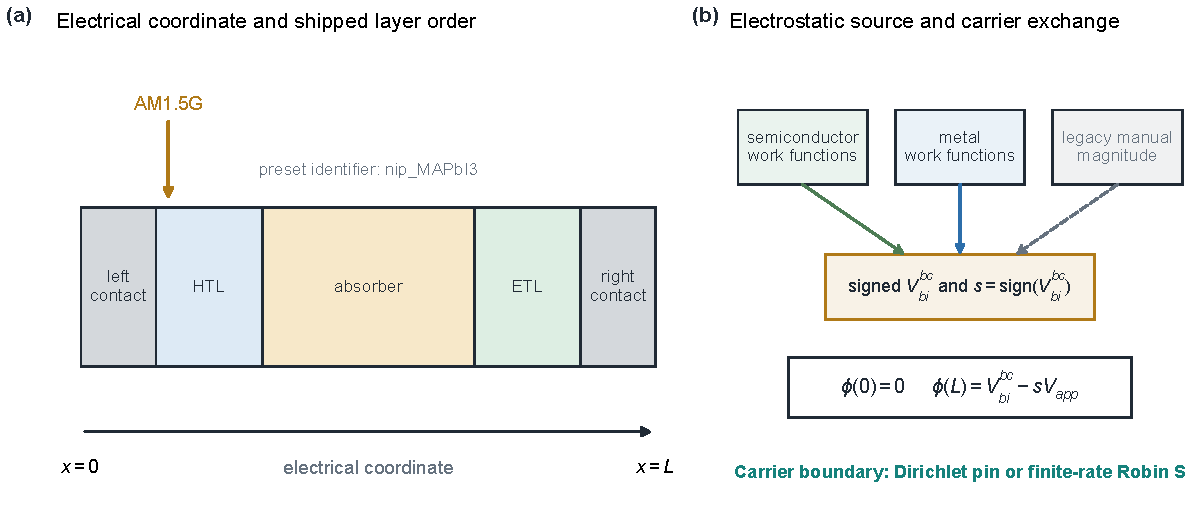
\includegraphics[width=0.98\textwidth,height=\textheight]{figures/device_contact_boundary.pdf}
\caption{Electrical coordinate, layer order, and contact-potential
sources}
\end{figure}

Illumination is always incident at \(x=0\), through the first listed
electrical layer after any optical-only substrate. The shipped
\texttt{nip\_MAPbI3} identifier therefore refers to a stored preset, not
to a rule for which transport layer faces the light. Its YAML order is
HTL, absorber, ETL. When porting a structure from the literature, check
the layer sequence and the \(x=0\) convention rather than inferring the
orientation from the preset name.

The Poisson contact potential and the carrier contact law are separate
inputs. New physical configurations obtain the signed contact potential
from endpoint semiconductor work functions or from two explicit metal
work functions. The manual magnitude remains only for legacy
comparisons. Carrier exchange is then set independently by Dirichlet
pins or finite-rate Robin velocities.

\begin{figure}
\centering
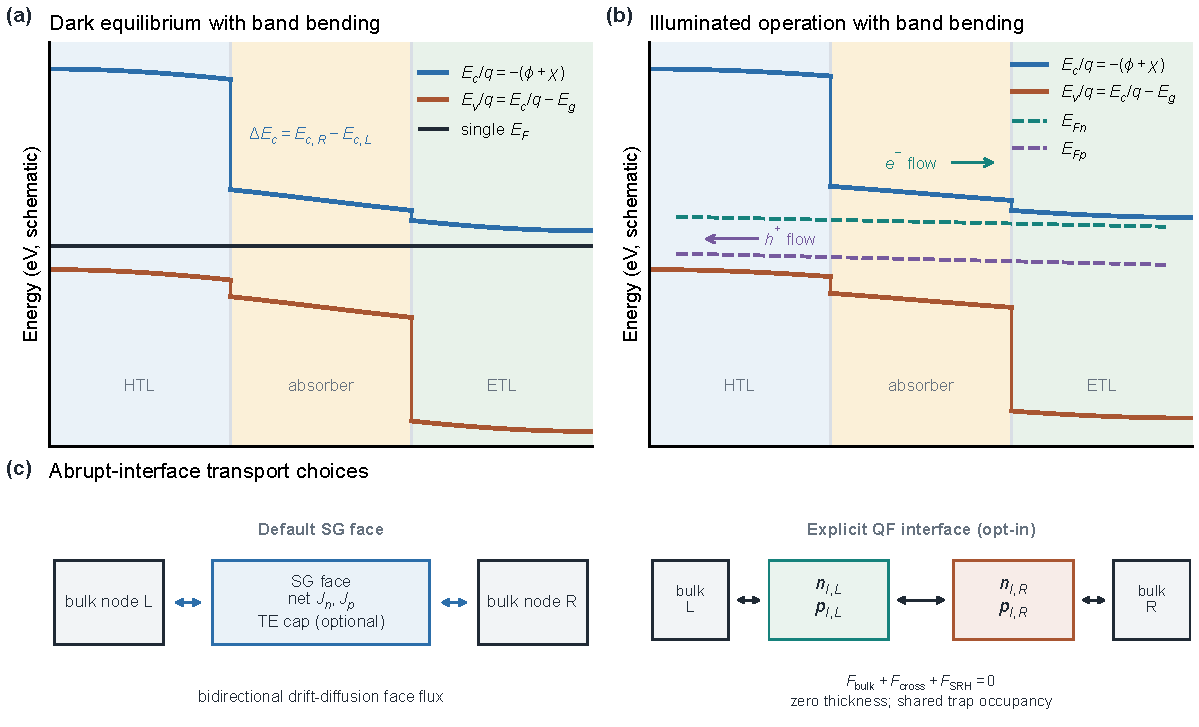
\includegraphics[width=0.98\textwidth,height=\textheight]{figures/band_interface_convention.pdf}
\caption{Band bending, quasi-Fermi levels, and abrupt-interface
closures}
\end{figure}

The first two panels are schematic energy profiles rather than output
from one particular device. They include a continuous electrostatic
potential so that the bands bend within each layer, while the affinity
and band-gap changes produce the abrupt offsets. At dark equilibrium
there is one flat Fermi level. Under illumination the electron and hole
quasi-Fermi levels split; the arrows show carrier motion toward the
selective contacts, not the conventional-current sign. The default
discretization uses one bidirectional Scharfetter-Gummel face whose
magnitude may be limited by the optional thermionic cap. The opt-in QF
boundary removes that face and balances bulk supply, reciprocal
cross-interface transport, and shared interface SRH on a zero-thickness
plane.

\hypertarget{beginner-physics-primer}{%
\chapter{Beginner Physics Primer}\label{beginner-physics-primer}}

\hypertarget{electrons-holes-and-bands}{%
\section{Electrons, Holes, And Bands}\label{electrons-holes-and-bands}}

In a semiconductor, electrons can move in the conduction band and holes
can move in the valence band. A solar cell works because light creates
electron-hole pairs and the device structure makes it more likely that
electrons leave through one contact while holes leave through the other.

SolarLab stores two energy parameters that are essential for
heterojunctions:

\begin{itemize}
\tightlist
\item
  \(\chi\), the electron affinity;
\item
  \(E_g\), the band gap.
\end{itemize}

Together these determine approximate conduction-band and valence-band
positions. At an interface, a change in \(\chi\) or \(E_g\) creates band
offsets. Band offsets are important because they can block one carrier
type while allowing the other carrier type to pass.

\hypertarget{generation-and-recombination}{%
\section{Generation And
Recombination}\label{generation-and-recombination}}

Optical generation \(G(x)\) is the rate at which absorbed photons create
electron-hole pairs per unit volume. Recombination \(R(n,p)\) is the
rate at which electrons and holes annihilate. A good solar cell has high
generation and carrier collection, but low recombination.

SolarLab includes several recombination channels:

\begin{itemize}
\tightlist
\item
  Shockley-Read-Hall (SRH) trap-assisted recombination;
\item
  radiative recombination;
\item
  Auger recombination;
\item
  interface recombination through surface recombination velocities;
\item
  optional trap-density profiles near interfaces.
\end{itemize}

\hypertarget{mobile-ions-and-hysteresis}{%
\section{Mobile Ions And Hysteresis}\label{mobile-ions-and-hysteresis}}

Perovskite cells can contain mobile ionic defects. These defects move
much more slowly than electronic carriers. During a voltage scan, the
ion profile may not reach equilibrium at each voltage. This creates J-V
hysteresis. SolarLab treats this as a physical transient, not as a
post-processing correction.

In the state vector, the default mobile ion variable is \(P\), the
positive vacancy density. A second negative species can be configured
through \texttt{D\_ion\_neg}, \texttt{P0\_neg}, and
\texttt{P\_lim\_neg}.

\hypertarget{device-definition}{%
\chapter{Device Definition}\label{device-definition}}

\hypertarget{core-data-flow}{%
\section{Core Data Flow}\label{core-data-flow}}

The simulator data flow is:

\begin{verbatim}
YAML or inline device dictionary
-> MaterialParams + LayerSpec + DeviceStack
-> experiment driver
-> MaterialArrays cache
-> result dataclass
\end{verbatim}

The main dataclasses are:

\begin{itemize}
\tightlist
\item
  \texttt{MaterialParams}: physical parameters for one material.
\item
  \texttt{LayerSpec}: layer name, role, thickness, and material
  parameters.
\item
  \texttt{DeviceStack}: full multilayer stack and global device
  settings.
\end{itemize}

\hypertarget{layer-roles}{%
\section{Layer Roles}\label{layer-roles}}

Layer roles used by the frontend and YAML schema are:

\begin{longtable}[]{@{}ll@{}}
\toprule
Role & Meaning \\
\midrule
\endhead
\texttt{substrate} & optical-only layer, excluded from electrical
drift-diffusion \\
\texttt{front\_contact} & front electrode or transparent conductor \\
\texttt{ETL} & electron transport layer \\
\texttt{absorber} & active photovoltaic absorber \\
\texttt{HTL} & hole transport layer \\
\texttt{back\_contact} & rear electrode \\
\bottomrule
\end{longtable}

Substrate layers must form a contiguous prefix of the stack. They
participate in transfer-matrix optics but do not appear in the
drift-diffusion grid.

\hypertarget{main-material-parameters}{%
\section{Main Material Parameters}\label{main-material-parameters}}

\begin{longtable}[]{@{}lll@{}}
\toprule
Field & Meaning & Unit \\
\midrule
\endhead
\texttt{eps\_r} & relative permittivity & dimensionless \\
\texttt{mu\_n}, \texttt{mu\_p} & electron and hole mobilities &
\(m^2 V^{-1} s^{-1}\) \\
\texttt{v\_th} & layer thermal velocity used by interface kinetics &
\(m\,s^{-1}\) \\
\texttt{D\_ion} & positive ion diffusion coefficient & \(m^2 s^{-1}\) \\
\texttt{P\_lim} & positive-ion finite-site density scale & \(m^{-3}\) \\
\texttt{P0} & initial positive ion density & \(m^{-3}\) \\
\texttt{ni} & intrinsic carrier density & \(m^{-3}\) \\
\texttt{tau\_n}, \texttt{tau\_p} & SRH lifetimes & \(s\) \\
\texttt{n1}, \texttt{p1} & SRH trap reference densities & \(m^{-3}\) \\
\texttt{B\_rad} & radiative recombination coefficient &
\(m^3 s^{-1}\) \\
\texttt{C\_n}, \texttt{C\_p} & Auger coefficients & \(m^6 s^{-1}\) \\
\texttt{alpha} & Beer-Lambert absorption coefficient & \(m^{-1}\) \\
\texttt{N\_A}, \texttt{N\_D} & acceptor and donor densities &
\(m^{-3}\) \\
\texttt{chi} & electron affinity & eV \\
\texttt{Eg} & band gap & eV \\
\texttt{Nc300}, \texttt{Nv300} & effective band-edge densities of states
at 300 K & \(m^{-3}\) \\
\texttt{A\_star\_n}, \texttt{A\_star\_p} & electron and hole Richardson
constants & \(A\,m^{-2}K^{-2}\) \\
\texttt{optical\_material} & key into \texttt{data/nk/*.csv} & string \\
\texttt{incoherent} & incoherent TMM layer flag & boolean \\
\bottomrule
\end{longtable}

Additional optional parameters cover negative ions, temperature scaling,
field-dependent mobility, trap profiles, and optical fallbacks.

\hypertarget{parameter-dictionary}{%
\section{Parameter Dictionary}\label{parameter-dictionary}}

Input specification is a dominant source of simulation error. SolarLab
cannot infer whether a parameter comes from measurement, literature,
fitting, or exploratory screening, so each field should be recorded with
its source and value.

\hypertarget{electrical-and-transport-fields}{%
\subsection{Electrical And Transport
Fields}\label{electrical-and-transport-fields}}

\begingroup\footnotesize\setlength{\tabcolsep}{3.5pt}

\renewcommand{\arraystretch}{1.18}
\begin{longtable}{@{}>{\raggedright\arraybackslash}p{0.20\linewidth}>{\raggedleft\arraybackslash}p{0.16\linewidth}>{\raggedright\arraybackslash}p{0.25\linewidth}>{\raggedright\arraybackslash}p{0.31\linewidth}@{}}
\toprule
Field & Unit & Physical role & Beginner guidance \\
\midrule
\endhead
\path{eps_r} & 1 & relative permittivity in Poisson's equation & Larger values screen charge and reduce field gradients. Use layer-specific literature values rather than a single generic perovskite value. \\
\path{mu_n} & \(m^2 V^{-1} s^{-1}\) & low-field electron mobility & Controls electron extraction and transport resistance. Remember that \(1\,cm^2 V^{-1}s^{-1}=10^{-4}\,m^2 V^{-1}s^{-1}\). \\
\path{mu_p} & \(m^2 V^{-1} s^{-1}\) & low-field hole mobility & Same unit conversion convention as \path{mu_n}. Low mobility typically affects FF before producing a large change in \(V_\mathrm{oc}\). \\
\path{v_th} & \(m\,s^{-1}\) & carrier thermal velocity supplied to SCAPS-style interface kinetics & The default is \(10^5\,m\,s^{-1}\). The SCAPS loader imports the declared per-layer value; do not confuse it with drift velocity or mobility. \\
\path{N_A} & \(m^{-3}\) & ionized acceptor density & Represents p-type doping. Values reported in \(cm^{-3}\) must be multiplied by \(10^6\). \\
\path{N_D} & \(m^{-3}\) & ionized donor density & Represents n-type doping. Use compensated doping only when it is part of the intended physical model. \\
\path{ni} & \(m^{-3}\) & intrinsic carrier density & Appears in mass action and SRH terms. It should be consistent with the effective band gap and temperature when doing parameter studies. \\
\path{chi} & eV & electron affinity & Sets approximate conduction-band alignment. Inconsistent \(\chi\) values can introduce artificial transport barriers. \\
\path{Eg} & eV & band gap & Sets band offsets and thermodynamic interpretation. Beer-Lambert optics do not automatically shift spectral absorption when \path{Eg} changes. \\
\path{A_star_n}, \path{A_star_p} & \(A\,m^{-2}K^{-2}\) & electron and hole Richardson supplies for interface-limited transport & The physical interface uses one reciprocal prefactor per carrier, selected conservatively from the adjacent layers. Keep these values consistent with the effective DOS or effective-mass assumption. \\
\bottomrule
\end{longtable}
\endgroup

\hypertarget{ion-and-hysteresis-fields}{%
\subsection{Ion And Hysteresis Fields}\label{ion-and-hysteresis-fields}}

\begingroup\footnotesize\setlength{\tabcolsep}{3.5pt}

\renewcommand{\arraystretch}{1.18}
\begin{longtable}{@{}>{\raggedright\arraybackslash}p{0.20\linewidth}>{\raggedleft\arraybackslash}p{0.16\linewidth}>{\raggedright\arraybackslash}p{0.25\linewidth}>{\raggedright\arraybackslash}p{0.31\linewidth}@{}}
\toprule
Field & Unit & Physical role & Beginner guidance \\
\midrule
\endhead
\path{D_ion} & \(m^2 s^{-1}\) & positive mobile-ion diffusion coefficient & Set to zero when mobile ions are excluded from the model. Nonzero values can produce scan-rate dependence. \\
\path{P0} & \(m^{-3}\) & initial positive ion density & Represents the equilibrium mobile-vacancy population before redistribution. \\
\path{P_lim} & \(m^{-3}\) & positive-ion finite-site density entering the crowding chemical potential & Use a physically motivated mobile-site density. It is not a hard transient-state projection. \\
\path{D_ion_neg} & \(m^2 s^{-1}\) & negative mobile-ion diffusion coefficient & Enables a second mobile species. Leave zero for the default single-ion model. \\
\path{P0_neg} & \(m^{-3}\) & initial negative ion density & Use only when the negative species is part of the physical hypothesis. \\
\path{P_lim_neg} & \(m^{-3}\) & negative-ion finite-site density scale & Same interpretation as \path{P_lim}; a shared-site model normally uses a common reservoir scale. \\
\path{E_a_ion} & eV & Arrhenius activation energy for ion diffusion & Used for temperature-dependent ion mobility. Fitted or literature-derived values should be reported with provenance. \\
\bottomrule
\end{longtable}
\endgroup

\hypertarget{recombination-and-trap-fields}{%
\subsection{Recombination And Trap
Fields}\label{recombination-and-trap-fields}}

\begingroup\footnotesize\setlength{\tabcolsep}{3.5pt}

\renewcommand{\arraystretch}{1.18}
\begin{longtable}{@{}>{\raggedright\arraybackslash}p{0.20\linewidth}>{\raggedleft\arraybackslash}p{0.16\linewidth}>{\raggedright\arraybackslash}p{0.25\linewidth}>{\raggedright\arraybackslash}p{0.31\linewidth}@{}}
\toprule
Field & Unit & Physical role & Beginner guidance \\
\midrule
\endhead
\path{tau_n} & s & electron SRH lifetime & Shorter lifetime increases trap-assisted recombination. It is often an effective fitted parameter. \\
\path{tau_p} & s & hole SRH lifetime & Interpret with \path{tau_n}; asymmetry can model carrier-selective trap response. \\
\path{n1} & \(m^{-3}\) & SRH electron reference density & Encodes the effective trap-energy position and should be changed consistently with the trap model. \\
\path{p1} & \(m^{-3}\) & SRH hole reference density & Companion to \path{n1}. \\
\path{B_rad} & \(m^3 s^{-1}\) & radiative recombination coefficient & Central to radiative-limit and photon-recycling studies. \\
\path{C_n} & \(m^6 s^{-1}\) & electron Auger coefficient & Most relevant when high carrier densities are expected. \\
\path{C_p} & \(m^6 s^{-1}\) & hole Auger coefficient & Same caution as \path{C_n}. \\
\path{trap_N_t_interface} & \(m^{-3}\) & interface-near trap density & Activates spatial trap profiles when supplied with decay information. \\
\path{trap_N_t_bulk} & \(m^{-3}\) & bulk trap density & The asymptotic trap density away from the interface. \\
\path{trap_decay_length} & m & decay length or Gaussian width & Must be physically resolvable by the grid. \\
\path{trap_profile_shape} & string & \path{exponential} or \path{gaussian} trap profile & Select the profile shape that corresponds to the assumed defect distribution. \\
\bottomrule
\end{longtable}
\endgroup

\hypertarget{optical-fields}{%
\subsection{Optical Fields}\label{optical-fields}}

\begingroup\footnotesize\setlength{\tabcolsep}{3.5pt}

\renewcommand{\arraystretch}{1.18}
\begin{longtable}{@{}>{\raggedright\arraybackslash}p{0.20\linewidth}>{\raggedleft\arraybackslash}p{0.16\linewidth}>{\raggedright\arraybackslash}p{0.25\linewidth}>{\raggedright\arraybackslash}p{0.31\linewidth}@{}}
\toprule
Field & Unit & Physical role & Beginner guidance \\
\midrule
\endhead
\path{alpha} & \(m^{-1}\) & scalar Beer-Lambert absorption coefficient & Suitable for simplified optical studies. It is not wavelength-resolved. \\
\path{optical_material} & string & key into tabulated \(n,k\) data & Required for TMM, EQE, and EL. The key must exist in \path{perovskite_sim/data/nk}. \\
\path{n_optical} & 1 & constant refractive-index fallback & Useful for approximate optical calculations but not a substitute for measured \(n,k\). \\
\path{incoherent} & boolean & thick-layer incoherent TMM treatment & Intended for the first thick substrate. The current TMM path does not support arbitrary incoherent layers mid-stack. \\
\bottomrule
\end{longtable}
\endgroup

\hypertarget{temperature-and-field-dependent-mobility-fields}{%
\subsection{Temperature And Field-Dependent Mobility
Fields}\label{temperature-and-field-dependent-mobility-fields}}

\begingroup\footnotesize\setlength{\tabcolsep}{3.5pt}

\renewcommand{\arraystretch}{1.18}
\begin{longtable}{@{}>{\raggedright\arraybackslash}p{0.20\linewidth}>{\raggedleft\arraybackslash}p{0.16\linewidth}>{\raggedright\arraybackslash}p{0.25\linewidth}>{\raggedright\arraybackslash}p{0.31\linewidth}@{}}
\toprule
Field & Unit & Physical role & Beginner guidance \\
\midrule
\endhead
\path{Nc300} & \(m^{-3}\) & conduction-band density of states at 300 K & Optional temperature-scaling input. Use only when the temperature model is calibrated. \\
\path{Nv300} & \(m^{-3}\) & valence-band density of states at 300 K & Companion to \path{Nc300}. \\
\path{mu_T_gamma} & 1 & mobility power-law temperature exponent & Default keeps a common scattering-style trend. Document any changed value. \\
\path{B_rad_T_gamma} & 1 & radiative coefficient temperature exponent & Default zero preserves legacy behavior. \\
\path{varshni_alpha} & eV K\(^{-1}\) & Varshni band-gap coefficient & Zero disables band-gap temperature shift. \\
\path{varshni_beta} & K & Varshni temperature parameter & Used with \path{varshni_alpha}. \\
\path{v_sat_n} & \(m\,s^{-1}\) & electron velocity-saturation limit & Zero disables Caughey-Thomas saturation for electrons. \\
\path{v_sat_p} & \(m\,s^{-1}\) & hole velocity-saturation limit & Zero disables Caughey-Thomas saturation for holes. \\
\path{ct_beta_n} & 1 & electron Caughey-Thomas exponent & Controls sharpness of velocity saturation. \\
\path{ct_beta_p} & 1 & hole Caughey-Thomas exponent & Same role for holes. \\
\path{pf_gamma_n} & \((V/m)^{-1/2}\) & electron Poole-Frenkel mobility coefficient & Zero disables field-enhanced hopping for electrons. \\
\path{pf_gamma_p} & \((V/m)^{-1/2}\) & hole Poole-Frenkel mobility coefficient & Zero disables field-enhanced hopping for holes. \\
\bottomrule
\end{longtable}
\endgroup

\hypertarget{device-level-fields}{%
\subsection{Device-Level Fields}\label{device-level-fields}}

\begingroup\footnotesize\setlength{\tabcolsep}{3.5pt}

\renewcommand{\arraystretch}{1.18}
\begin{longtable}{@{}>{\raggedright\arraybackslash}p{0.20\linewidth}>{\raggedleft\arraybackslash}p{0.16\linewidth}>{\raggedright\arraybackslash}p{0.25\linewidth}>{\raggedright\arraybackslash}p{0.31\linewidth}@{}}
\toprule
Field & Unit & Physical role & Beginner guidance \\
\midrule
\endhead
\path{built_in_potential_mode} & string & source of the signed Poisson contact potential & Use \path{semiconductor_work_function} or \path{metal_work_function} for new physical configurations. \\
\path{work_function_left_eV}, \path{work_function_right_eV} & eV & left and right metal work functions below vacuum & Required together in \path{metal_work_function} mode. \\
\path{V_bi_override} & V & legacy manual magnitude & Valid only in \path{legacy_manual}; use it for a frozen benchmark, not as a fitted default. \\
\path{V_bi} & V & deprecated compatibility input & Retained so shipped and imported benchmark files keep their recorded boundary condition. \\
\path{Phi} & \(m^{-2}s^{-1}\) & incident photon flux for Beer-Lambert generation & For spectral experiments use TMM data rather than only changing \path{Phi}. \\
\path{T} & K & device temperature & Affects thermal voltage and enabled temperature-dependent hooks. \\
\path{mode} & string & \path{legacy}, \path{fast}, or \path{full} physics tier & The mode is a ceiling; hooks still need required parameters. \\
\path{electrical_grid} & object & optional per-layer interval weights and tanh clustering strengths & Both maps must cover every electrical layer exactly. The global \path{N_grid} budget is retained. \\
\path{jv_solver_policy} & string & production J-V variable-set requirement & \path{general} permits the established drivers; \path{cancellation_safe_qf_required} rejects an uncertified driver unless a diagnostic override is explicit. \\
\path{interfaces} & \(m\,s^{-1}\) pairs & interface recombination velocities & One pair per internal electrical interface, ordered from the front contact toward the rear contact. \\
\path{S_n_left} & \(m\,s^{-1}\) & left electron contact velocity & \path{None} gives ohmic default. \path{0} is blocking. Large values approach ohmic extraction. \\
\path{S_p_left} & \(m\,s^{-1}\) & left hole contact velocity & Same convention as \path{S_n_left}. \\
\path{S_n_right} & \(m\,s^{-1}\) & right electron contact velocity & Same convention as \path{S_n_left}. \\
\path{S_p_right} & \(m\,s^{-1}\) & right hole contact velocity & Same convention as \path{S_n_left}. \\
\path{microstructure} & object & 2D grain-boundary specification & Used by 2D drivers; ignored by standard 1D paths. \\
\bottomrule
\end{longtable}
\endgroup

\hypertarget{advanced-model-options}{%
\subsection{Advanced Model Options}\label{advanced-model-options}}

These public \texttt{DeviceStack} fields change the equations or
determine which solver paths are available. The defaults below apply to
a new device. The \texttt{legacy} tier changes a few of them when an
older benchmark must be reproduced without altering its original setup.

\begingroup\footnotesize\setlength{\tabcolsep}{3.5pt}

\renewcommand{\arraystretch}{1.18}
\begin{longtable}{@{}>{\raggedright\arraybackslash}p{0.28\linewidth}>{\raggedright\arraybackslash}p{0.13\linewidth}>{\raggedright\arraybackslash}p{0.51\linewidth}@{}}
\toprule
Field & Default & Effect \\
\midrule
\endhead
\path{dos_band_potentials} & true & folds per-layer effective DOS into the Boltzmann transport potentials; legacy mode disables it \\
\path{te_physical_norm} & false & replaces the empirical density-weighted TE cap with a dimensionally normalized emission-velocity form; it remains opt-in while convergence is being extended for strongly binding interfaces \\
\path{ion_steric_diffusion_only} & true & selects the modified-PNP lattice-gas flux of Eq. \ref{eq:ion-flux}; false selects the legacy whole-flux regularization \\
\path{ion_steric_shared_site} & true & couples positive and negative mobile species through one finite-site reservoir when dual-ion mode is active \\
\path{flat_band_contacts} & false & activates the historical finite-rate Robin contact path; with an explicit potential mode it does not select the Poisson voltage \\
\path{flat_band_metal_contacts}, \path{contact_phi_B_eV} & false, 0 & optional majority-reservoir floor for weakly doped contacts; the barrier input is separate from the two explicit metal work functions \\
\path{interface_plane_projection} & false & uses the interface-sampling projection from older SCAPS comparisons; the physical QF interface uses a separate boundary formulation \\
\path{interface_two_sided} & false & older two-sided cross-carrier interface capture approximation \\
\path{interface_shared_occupancy} & false & older shared-occupancy interface-state approximation \\
\path{interface_plane_closure} & false & older supply-limited QSS plane-recombination support while retaining established SG transport \\
\path{interface_plane_generation} & false & allows signed generation on the older plane closure when its detailed-balance reference is physical \\
\path{het_recomb_despike} & 0 & SCAPS-emulation blend for an interface-node bulk-recombination spike; zero keeps the unmodified physical discretization \\
\path{band_grading} & false & activates the declared per-layer \path{Eg_back}/\path{chi_back} grading law and associated mesh refinement \\
\path{interface_tunneling}, \path{tunnel_mass_eff} & false, 0.2 & enables the static Padovani-Stratton enhancement at TE-capped faces and sets its effective mass \\
\bottomrule
\end{longtable}
\endgroup

The QF driver owns \path{interface_boundary},
\path{interface_transport_model}, and the QF coordinate choice; they are
not \texttt{DeviceStack} fields. These settings activate the boundary in
Eq.\textasciitilde{}\ref{eq:physical-interface-qss} only for
\path{quasi_fermi}. An unsupported combination raises an error.
\path{perovskite_sim/models/config_loader.py} defines the accepted YAML
keys; the table lists public physical options and omits private cache
fields.

\hypertarget{global-device-parameters}{%
\section{Global Device Parameters}\label{global-device-parameters}}

The device-level YAML maps to the following \texttt{DeviceStack} fields.
The legacy manual voltage is the only field whose public YAML name
differs from its runtime storage name:

\begingroup\footnotesize\setlength{\tabcolsep}{3.5pt}

\renewcommand{\arraystretch}{1.18}
\begin{longtable}{@{}>{\raggedright\arraybackslash}p{0.34\linewidth}>{\raggedright\arraybackslash}p{0.58\linewidth}@{}}
\toprule
Field & Meaning \\
\midrule
\endhead
\path{built_in_potential_mode} & \path{semiconductor_work_function}, \path{metal_work_function}, or \path{legacy_manual} \\
\path{work_function_left_eV}, \path{work_function_right_eV} & explicit metal work functions for the two contacts \\
\path{V_bi_override} (YAML) $\rightarrow$ \path{V_bi} (runtime) & manual magnitude used only by the explicit legacy mode \\
\path{V_bi} (YAML) & deprecated alias retained for unmodified compatibility presets \\
\path{Phi} & incident photon flux for Beer-Lambert generation \\
\path{interfaces} & interface recombination velocities \((v_n,v_p)\) \\
\path{T} & device temperature in K \\
\path{mode} & \path{legacy}, \path{fast}, or \path{full} \\
\path{grid_interval_weights}, \path{grid_alphas} & optional electrical-grid allocation and per-layer clustering controls \\
\path{jv_solver_policy} & \path{general} or \path{cancellation_safe_qf_required} \\
\path{S_n_left}, \path{S_p_left}, \path{S_n_right}, \path{S_p_right} & selective-contact velocities \\
\path{microstructure} & optional 2D grain-boundary block \\
\bottomrule
\end{longtable}
\endgroup

\hypertarget{built-in-potential}{%
\section{Built-In Potential}\label{built-in-potential}}

In a new physical device file, SolarLab calculates the built-in
potential from the equilibrium contact-potential difference,

\[
V_\mathrm{bi}=\phi(L)-\phi(0)=W_\mathrm{left}-W_\mathrm{right},
\]

where each \(W\) is measured downward from vacuum and entered as a
positive energy. \path{built_in_potential_mode} selects how
\(W_\mathrm{left}\) and \(W_\mathrm{right}\) are supplied:

\begin{itemize}
\item
  \texttt{semiconductor\_work\_function} derives each contact work
  function from the outer electrical layer. It requires positive
  \(\chi\), \(E_g\), \(N_{C,300}\) and \(N_{V,300}\) on both contact
  layers, together with finite non-negative doping. For
  Maxwell-Boltzmann statistics,

  \[
  W_n=\chi+V_T\ln\!\left(\frac{N_C}{n}\right),\qquad
  W_p=\chi+E_g-V_T\ln\!\left(\frac{N_V}{p}\right),
  \]

  with \(n\) or \(p\) obtained from charge neutrality and mass action.
  The active temperature law supplies \(N_C(T)\), \(N_V(T)\) and the
  optional Varshni shift; contact-face doping and band grading are
  included. Loading stops if the DOS or band data needed for this
  calculation are missing.
\item
  \path{metal_work_function} uses the measured or specified electrode
  values \path{work_function_left_eV} and \path{work_function_right_eV}
  directly. Use this mode when the electrodes are specified as metals.
\item
  \path{legacy_manual} accepts a non-negative \path{V_bi_override}
  magnitude. The field direction still follows the endpoint junction
  orientation. Use it only for a frozen benchmark or imported protocol
  in which the manual voltage is part of the reference definition. New
  physical devices should use one of the two work-function modes.
\end{itemize}

SolarLab keeps the sign of the result. It is positive for the usual
p-contact-left orientation and negative for an n-contact-left stack such
as an n-window/p-absorber CIGS cell or an n\(^+\)/p silicon junction. Do
not apply \texttt{abs()} at the Poisson boundary. The applied-voltage
polarity is handled separately, so positive forward bias reduces the
field magnitude in either orientation:

\[
\phi(0)=\phi_\mathrm{left}, \qquad
\phi(L)=\phi_\mathrm{left}+V_\mathrm{bi}
-\operatorname{sgn}(V_\mathrm{bi})V_\mathrm{app}.
\]

With an explicit potential mode, \texttt{flat\_band\_contacts} affects
only finite-rate Robin carrier exchange at the two outer contacts; the
four \texttt{S\_*} fields refine those rates. It leaves the Poisson
voltage unchanged. The selected contact densities and potential must
still be checked for dark-equilibrium consistency.

With doping-derived ohmic pins, a common dark quasi-Fermi level requires

\[
V_\mathrm{bi}=W_{s,\mathrm{left}}-W_{s,\mathrm{right}},
\]

where the semiconductor work functions \(W_s\) use the same contact-face
bands, DOS, doping and temperature as the pinned densities.
\path{semiconductor_work_function} meets this condition by construction.
In \path{metal_work_function} mode, the reservoir or Schottky barrier
must also agree with the stated metal work function and adjacent band
edge. Ordinary doping pins are suitable only when they describe the same
effective reservoir; otherwise \(V_\mathrm{app}=0\) can retain a contact
quasi-Fermi mismatch even though the Poisson voltage is well defined.
The optional \texttt{flat\_band\_metal\_contacts} floor uses the
separate \texttt{contact\_phi\_B\_eV} input; it is not inferred from the
two metal work functions.

\begin{longtable}[]{@{}
  >{\raggedright\arraybackslash}p{(\columnwidth - 4\tabcolsep) * \real{0.33}}
  >{\raggedright\arraybackslash}p{(\columnwidth - 4\tabcolsep) * \real{0.33}}
  >{\raggedright\arraybackslash}p{(\columnwidth - 4\tabcolsep) * \real{0.33}}@{}}
\toprule
Potential source & Carrier boundary & Interpretation \\
\midrule
\endhead
\path{semiconductor_work_function} & doping-derived ohmic pins &
recommended ideal semiconductor-reservoir pair; dark-equilibrium
compatible under the stated Maxwell-Boltzmann assumptions \\
\path{metal_work_function} & work-function-consistent Robin/Schottky
reservoir & physical metal-contact pair when the barrier and exchange
velocities have independent provenance \\
\path{metal_work_function} & unchanged doping-derived pins & valid only
if the two reservoirs are demonstrably equivalent; otherwise diagnostic
or calibrated rather than an automatic equilibrium \\
\path{legacy_manual} & historical benchmark contacts & use only to
reproduce the recorded benchmark; it does not define a new physical
contact model \\
\bottomrule
\end{longtable}

For a new contact model, verify zero dark current, spatially constant
equilibrium quasi-Fermi levels and mesh convergence before using
illuminated figures of merit.

Older files keep their original loading behavior. A device block
containing \path{V_bi} but no \path{built_in_potential_mode} follows the
historical compatibility rule, including the old
\path{flat_band_contacts} implication. The shipped IonMonger and
Driftfusion benchmarks therefore retain their recorded manual values.
Saving the file without changing the selector preserves its old shape;
selecting an explicit physical mode removes the manual field. For
example, the IonMonger reference records \(1.10\) V, while its
incomplete legacy band construction gives about \(0.86\) V. Substituting
\(0.86\) V would define a different benchmark.

\hypertarget{yaml-example}{%
\section{YAML Example}\label{yaml-example}}

\begin{Shaded}
\begin{Highlighting}[]
\FunctionTok{device}\KeywordTok{:}
\AttributeTok{  }\FunctionTok{built\_in\_potential\_mode}\KeywordTok{:}\AttributeTok{ metal\_work\_function}
\AttributeTok{  }\FunctionTok{work\_function\_left\_eV}\KeywordTok{:}\AttributeTok{ }\FloatTok{5.20}
\AttributeTok{  }\FunctionTok{work\_function\_right\_eV}\KeywordTok{:}\AttributeTok{ }\FloatTok{4.10}
\AttributeTok{  }\FunctionTok{Phi}\KeywordTok{:}\AttributeTok{ }\FloatTok{2.5e21}
\AttributeTok{  }\FunctionTok{T}\KeywordTok{:}\AttributeTok{ }\FloatTok{300.0}
\AttributeTok{  }\FunctionTok{mode}\KeywordTok{:}\AttributeTok{ full}
\AttributeTok{  }\FunctionTok{contacts}\KeywordTok{:}
\AttributeTok{    }\FunctionTok{left}\KeywordTok{:}
\AttributeTok{      }\FunctionTok{S\_p}\KeywordTok{:}\AttributeTok{ }\FloatTok{1.0e3}
\AttributeTok{      }\FunctionTok{S\_n}\KeywordTok{:}\AttributeTok{ }\FloatTok{1.0e{-}3}
\AttributeTok{    }\FunctionTok{right}\KeywordTok{:}
\AttributeTok{      }\FunctionTok{S\_n}\KeywordTok{:}\AttributeTok{ }\FloatTok{1.0e3}
\AttributeTok{      }\FunctionTok{S\_p}\KeywordTok{:}\AttributeTok{ }\FloatTok{1.0e{-}3}

\FunctionTok{electrical\_grid}\KeywordTok{:}
\AttributeTok{  }\FunctionTok{interval\_weights}\KeywordTok{:}\CommentTok{       \# one positive weight per electrical layer}
\AttributeTok{    }\FunctionTok{HTL}\KeywordTok{:}\AttributeTok{ }\FloatTok{1.0}
\AttributeTok{  }\FunctionTok{alphas}\KeywordTok{:}\CommentTok{                 \# per{-}layer tanh clustering strength}
\AttributeTok{    }\FunctionTok{HTL}\KeywordTok{:}\AttributeTok{ }\FloatTok{3.0}

\FunctionTok{layers}\KeywordTok{:}
\AttributeTok{  }\KeywordTok{{-}}\AttributeTok{ }\FunctionTok{name}\KeywordTok{:}\AttributeTok{ HTL}
\AttributeTok{    }\FunctionTok{role}\KeywordTok{:}\AttributeTok{ HTL}
\AttributeTok{    }\FunctionTok{thickness}\KeywordTok{:}\AttributeTok{ }\FloatTok{2.0e{-}7}
\AttributeTok{    }\FunctionTok{eps\_r}\KeywordTok{:}\AttributeTok{ }\FloatTok{3.0}
\AttributeTok{    }\FunctionTok{mu\_n}\KeywordTok{:}\AttributeTok{ }\FloatTok{1.0e{-}8}
\AttributeTok{    }\FunctionTok{mu\_p}\KeywordTok{:}\AttributeTok{ }\FloatTok{1.0e{-}6}
\AttributeTok{    }\FunctionTok{ni}\KeywordTok{:}\AttributeTok{ }\FloatTok{1.0e9}
\AttributeTok{    }\FunctionTok{N\_A}\KeywordTok{:}\AttributeTok{ }\FloatTok{1.0e24}
\AttributeTok{    }\FunctionTok{N\_D}\KeywordTok{:}\AttributeTok{ }\FloatTok{0.0}
\AttributeTok{    }\FunctionTok{D\_ion}\KeywordTok{:}\AttributeTok{ }\FloatTok{0.0}
\AttributeTok{    }\FunctionTok{P\_lim}\KeywordTok{:}\AttributeTok{ }\FloatTok{1.0e27}
\AttributeTok{    }\FunctionTok{P0}\KeywordTok{:}\AttributeTok{ }\FloatTok{0.0}
\AttributeTok{    }\FunctionTok{tau\_n}\KeywordTok{:}\AttributeTok{ }\FloatTok{1.0e{-}6}
\AttributeTok{    }\FunctionTok{tau\_p}\KeywordTok{:}\AttributeTok{ }\FloatTok{1.0e{-}6}
\AttributeTok{    }\FunctionTok{n1}\KeywordTok{:}\AttributeTok{ }\FloatTok{1.0e9}
\AttributeTok{    }\FunctionTok{p1}\KeywordTok{:}\AttributeTok{ }\FloatTok{1.0e9}
\AttributeTok{    }\FunctionTok{B\_rad}\KeywordTok{:}\AttributeTok{ }\FloatTok{0.0}
\AttributeTok{    }\FunctionTok{C\_n}\KeywordTok{:}\AttributeTok{ }\FloatTok{0.0}
\AttributeTok{    }\FunctionTok{C\_p}\KeywordTok{:}\AttributeTok{ }\FloatTok{0.0}
\AttributeTok{    }\FunctionTok{alpha}\KeywordTok{:}\AttributeTok{ }\FloatTok{0.0}
\AttributeTok{    }\FunctionTok{chi}\KeywordTok{:}\AttributeTok{ }\FloatTok{2.2}
\AttributeTok{    }\FunctionTok{Eg}\KeywordTok{:}\AttributeTok{ }\FloatTok{3.0}
\end{Highlighting}
\end{Shaded}

For semiconductor-derived contacts, set \path{built_in_potential_mode}
to \path{semiconductor_work_function} and provide \texttt{Nc300} and
\texttt{Nv300} on both outer electrical layers. A frozen manual
benchmark should state its exception rather than look like a physical
default:

\begin{Shaded}
\begin{Highlighting}[]
\FunctionTok{device}\KeywordTok{:}
\AttributeTok{  }\FunctionTok{built\_in\_potential\_mode}\KeywordTok{:}\AttributeTok{ legacy\_manual}
\AttributeTok{  }\FunctionTok{V\_bi\_override}\KeywordTok{:}\AttributeTok{ }\FloatTok{1.10}
\end{Highlighting}
\end{Shaded}

The old key \texttt{V\_bi} remains readable only for unmodified
compatibility files.

YAML 1.1 can parse bare scientific notation such as \texttt{1e-9} as a
string. SolarLab coerces numeric-looking strings to floats, but writing
values as \texttt{1.0e-9} is clearer and safer.

\hypertarget{governing-equations}{%
\chapter{Governing Equations}\label{governing-equations}}

This chapter states the governing equations in dimensional SI form. The
model belongs to the class of coupled Poisson/drift-diffusion (van
Roosbroeck) systems, extended by Nernst-Planck transport for mobile
ionic defects, heterojunction band alignment, and wavelength-resolved
optical generation. The implementation evaluates discretized node and
face arrays (Chapter \ref{numerical-method}), but the continuous form
stated here clarifies the model assumptions and the physical meaning of
each state variable.

Throughout, \(q\) is the elementary charge, \(k_B\) Boltzmann's
constant, \(T\) the lattice temperature, and \(V_T = k_B T/q\) the
thermal voltage. Bulk carrier statistics are Maxwell-Boltzmann
(non-degenerate). The opt-in physical interface boundary alone uses
bounded Fermi occupations at the two band edges to keep its
zero-thickness plane states below their available densities of states;
this does not turn the bulk model into a Fermi-Dirac transport model.

\hypertarget{electrostatics-the-poisson-equation}{%
\section{Electrostatics: The Poisson
Equation}\label{electrostatics-the-poisson-equation}}

The electrostatic potential \(\phi(x,t)\) is obtained from the
quasistatic Poisson equation

\begin{equation}
\label{eq:poisson}
\frac{\partial}{\partial x}
\left(
\varepsilon_0 \varepsilon_r
\frac{\partial \phi}{\partial x}
\right)
= -\rho ,
\end{equation}

with the space-charge density assembled from every charged species in
the model:

\begin{equation}
\label{eq:charge-density}
\rho
=
q\left[
p - n + \left(P - P_0\right) - \left(P^- - P^-_0\right)
+ N_D - N_A
\right].
\end{equation}

The mobile-ion contributions are measured relative to their neutral
background densities \(P_0\) and \(P^-_0\): an undisturbed vacancy
population together with its immobile counter-charge is electrically
neutral, so only the \emph{redistribution} of ions contributes net space
charge. The negative-species term is present only when a second mobile
species is configured (dual-ion mode).

The quasistatic approximation asserts that the potential responds
instantaneously to the charge configuration --- Eq. \ref{eq:poisson} is
Gauss's law
\(\nabla\cdot(\varepsilon_0\varepsilon_r \mathbf{E}) = \rho\) with
\(E = -\partial\phi/\partial x\), solved at every instant of the
transient. Retardation, magnetic effects, and electromagnetic wave
propagation are excluded from the electrical solve (the optical field is
treated separately by the transfer-matrix machinery of the \emph{Optical
Generation} section).

The discretization is finite-volume with a harmonic-mean face
permittivity:

\begin{equation}
\label{eq:harmonic-eps}
\varepsilon_{i+1/2}
=
\frac{2\varepsilon_i\varepsilon_{i+1}}
{\varepsilon_i+\varepsilon_{i+1}} .
\end{equation}

When the material interface falls at the midpoint between the two nodes,
the harmonic mean is the exact series composition of the two dielectric
half-cells: it is the face permittivity for which the discrete flux
reproduces a continuous normal displacement
\(D = \varepsilon_0\varepsilon_r E\) across the discontinuity, with the
field jumping between the layers as it physically must. An arithmetic
(nodal) mean is the \emph{parallel} composition instead, which is the
correct average for a face-tangential field, so using it here
misallocates the potential drop between the two layers. Neither choice
literally imposes a boundary condition on \(E\); the difference is which
equivalent series-versus-parallel dielectric response the face flux
represents.

For a general non-symmetric geometry, where the interface does not sit
at the midpoint, the correct series composition is the
\emph{distance-weighted} harmonic mean

\[
\varepsilon_f=
\frac{\Delta x_L+\Delta x_R}
{\Delta x_L/\varepsilon_L+\Delta x_R/\varepsilon_R},
\]

which reduces to Eq. \ref{eq:harmonic-eps} for equal half-widths.
SolarLab places every material interface \emph{on} a grid node and
assigns that node the permittivity of the layer to its right, so each
face lies entirely within one material and Eq. \ref{eq:harmonic-eps}
smears the discontinuity over one half-cell rather than weighting two
dissimilar half-cells. This is the usual node-centred finite-volume
treatment and its error is first order in the local cell width; it is
\emph{not} a distance-weighting bug, but it does mean the interface is
resolved to within half a cell, so interface-sensitive quantities should
be checked for mesh convergence.

Assumptions and limits:

\begin{itemize}
\tightlist
\item
  electrostatics is quasistatic;
\item
  magnetic effects and wave propagation in the electrical solve are
  ignored;
\item
  layer interfaces are abrupt on the scale of the grid;
\item
  \(\rho\) is built from the configured mobile species, carriers, and
  dopants, with dopants assumed fully ionized and immobile.
\end{itemize}

\hypertarget{carrier-transport-continuity-and-drift-diffusion}{%
\section{Carrier Transport: Continuity And
Drift-Diffusion}\label{carrier-transport-continuity-and-drift-diffusion}}

The electron and hole densities obey the continuity equations

\begin{equation}
\label{eq:electron-continuity}
\frac{\partial n}{\partial t}
=
\frac{1}{q}\frac{\partial J_n}{\partial x}
+G-R ,
\end{equation}

\begin{equation}
\label{eq:hole-continuity}
\frac{\partial p}{\partial t}
=
-\frac{1}{q}\frac{\partial J_p}{\partial x}
+G-R ,
\end{equation}

closed by the drift-diffusion constitutive relations

\begin{equation}
\label{eq:dd-currents}
J_n = q\mu_n n E + qD_n\frac{\partial n}{\partial x},
\qquad
J_p = q\mu_p p E - qD_p\frac{\partial p}{\partial x},
\end{equation}

with the Einstein relation \(D = \mu V_T\) linking diffusivity and
mobility. The Einstein relation expresses local thermal equilibrium
between the carrier gas and the lattice; it is exact for non-degenerate
(Boltzmann) statistics.

An equivalent and physically transparent form writes each current as a
quasi-Fermi-level gradient,

\begin{equation}
\label{eq:qfl-currents}
J_n = \mu_n\, n\, \frac{\partial E_{Fn}}{\partial x},
\qquad
J_p = \mu_p\, p\, \frac{\partial E_{Fp}}{\partial x},
\end{equation}

where, under Boltzmann statistics,
\(n = N_C \exp[-(E_C - E_{Fn})/k_BT]\) and
\(p = N_V \exp[-(E_{Fp} - E_V)/k_BT]\). Equations \ref{eq:dd-currents}
and \ref{eq:qfl-currents} are the same model; the quasi-Fermi form makes
explicit that a flat quasi-Fermi level implies zero current \emph{for
that carrier} --- the thermodynamic-equilibrium condition. At open
circuit only the net terminal current is constrained to zero: internal
electron and hole currents remain individually non-zero and convert into
each other through generation and recombination, so the quasi-Fermi
levels need not be flat everywhere in an operating device.

\hypertarget{heterojunction-band-alignment}{%
\subsection{Heterojunction Band
Alignment}\label{heterojunction-band-alignment}}

Band edges are referenced to the local vacuum level through the electron
affinity \(\chi\) and the band gap \(E_g\):

\[
E_C/q = -(\phi + \chi),
\qquad
E_V/q = -(\phi + \chi + E_g),
\]

with \(\chi\) and \(E_g\) expressed in volts (numerically equal to their
eV values). In heterojunction stacks SolarLab therefore drives the
carrier fluxes with \emph{band-effective} potentials,

\begin{equation}
\label{eq:band-corrected-potentials}
\phi_n=\phi+\chi, \qquad
\phi_p=\phi+\chi+E_g ,
\end{equation}

so that electrons respond to gradients of the conduction band edge and
holes to gradients of the valence band edge. An abrupt change in
\(\chi\) or \(E_g\) between layers then produces Anderson-rule band
offsets (\(\Delta E_C\) from the affinity step, \(\Delta E_V\) from the
combined affinity-plus-gap step) inside the same numerical flux
formulation, with no special-case interface treatment in the
discretization.

\hypertarget{effective-density-of-states-correction}{%
\subsection{Effective-Density-of-States
Correction}\label{effective-density-of-states-correction}}

For a heterostructure with unequal effective densities of states, the
band-effective potentials of Eq. \ref{eq:band-corrected-potentials} are
incomplete. Under Boltzmann statistics the carrier density couples to
the quasi-Fermi level through the local \(N_C\) or \(N_V\), so the exact
drift potentials carry an additional logarithmic term:

\begin{equation}
\label{eq:dos-potentials}
\phi_n = \phi + \chi + V_T\ln\!\frac{N_C}{N_C^{\mathrm{ref}}},
\qquad
\phi_p = \phi + \chi + E_g - V_T\ln\!\frac{N_V}{N_V^{\mathrm{ref}}} .
\end{equation}

Omitting these terms imposes a spurious quasi-Fermi-level discontinuity
of \(k_BT\,\ln(N_{C,1}/N_{C,2})\) (and the \(N_V\) analogue) at every
interface with a density-of-states contrast --- on a representative
HTL/perovskite/ETL stack the accumulated error exceeds 100 mV of
open-circuit voltage. SolarLab therefore folds the corrections of Eq.
\ref{eq:dos-potentials} into the cached per-layer \(\chi\)/\(E_g\)
arrays at build time, using the absorber as the reference layer (only
cross-junction \emph{differences} matter). The fold applies to transport
and thermionic emission only; purely statistical quantities (\(n_i\),
the SRH references \(n_1\)/\(p_1\), and the contact equilibrium
densities) are left unchanged. The correction is active by default
whenever per-layer \texttt{Nc300}/\texttt{Nv300} data are supplied, and
is disabled in the \texttt{legacy} tier, which reproduces the IonMonger
convention without DOS-folded transport.

Assumptions and limits:

\begin{itemize}
\tightlist
\item
  carriers are described by drift-diffusion transport, not ballistic
  transport;
\item
  carrier statistics are non-degenerate (Maxwell-Boltzmann);
  degenerately doped layers would require Fermi-Dirac corrections that
  are out of scope;
\item
  the model is most natural when local quasi-equilibrium is a reasonable
  approximation;
\item
  strongly quantum-confined structures, tunneling-dominated contacts,
  and hot carrier effects require additional modeling beyond this
  implementation.
\end{itemize}

\hypertarget{heterointerface-thermionic-emission-and-tunnelling}{%
\section{Heterointerface Thermionic Emission And
Tunnelling}\label{heterointerface-thermionic-emission-and-tunnelling}}

The drift-diffusion picture assumes that the band edges vary smoothly on
the scale of a grid cell. At an abrupt heterojunction the band offset is
instead resolved within a \emph{single} cell. With the band offsets and
density-of-states corrections carried in the exponentially fitted
potentials, the Scharfetter-Gummel flux (Chapter \ref{numerical-method})
is then the ideal-interface limit: it assumes local equilibrium across
the step and unlimited interface transmission, i.e.~no additional
kinetic resistance at the junction. That is an upper bound on the
transport a real interface supports whenever interface scattering, a
finite emission velocity, tunnelling, or interface-state supply actually
limit it --- it is not a systematic discretization error for every band
step, and the size of the discrepancy is a property of the interface,
not of the scheme. SolarLab therefore bounds the drift-diffusion face
flux by an interface-limited thermionic-emission (TE) flux of
Richardson-Dushman form at every face where the conduction- or
valence-band offset exceeds 50 meV:

\begin{equation}
\label{eq:te-flux}
J_{\mathrm{TE}}
\;\propto\;
A^{*}T^{2}
\left[
n_{L}\, e^{-\max(\Delta E,\,0)/V_T}
-
n_{R}\, e^{-\max(-\Delta E,\,0)/V_T}
\right],
\end{equation}

where \(\Delta E\) is the band-edge step across the face, \(n_L\) and
\(n_R\) are the adjacent carrier densities, and \(A^{*}\) is a per-face
Richardson constant (default: the free-electron value
\(1.2017\times10^{6}\,A\,m^{-2}K^{-2}\), overridable per layer). Only
the \emph{uphill} term carries the Boltzmann barrier penalty; a downhill
offset leaves the emission term unpenalized, so carriers flowing down a
band step are not artificially blocked.

Two points are important when using the default form. The
density-weighted form of Eq. \ref{eq:te-flux} is an \emph{empirical
interface-limited bound}. It is not the dimensional Richardson-Dushman
current: \(A^{*}T^{2}\) is already a current density, so multiplying by
an absolute carrier density leaves the bound's magnitude tied to the SI
unit system. This makes \(|J_{TE}|\) very large (order
\(10^{28}\)--\(10^{35}\) on a perovskite stack), so the
smaller-magnitude cap is rarely active; the observed heterojunction
\(V_\mathrm{oc}\) behaviour is driven by the band-offset potentials of
Eqs. \ref{eq:band-corrected-potentials}--\ref{eq:dos-potentials}, not by
the TE cap. A dimensionally correct \emph{emission-velocity} form is
available as an opt-in (\texttt{te\_physical\_norm}): dividing Eq.
\ref{eq:te-flux} by the band-edge density of states converts
\(A^{*}T^{2}\) into an emission velocity \(v_R = A^{*}T^{2}/(qN_C)\),
giving \(J = qv_R(\dots)\), which binds at real interface densities. The
normalized cap gives \(V_\mathrm{oc}=1.2013\,\mathrm{V}\) on the
mirrored regression configuration, the same value as the legacy cap
after correcting the cap direction and barrier input. It remains opt-in
because the coupled density solve still loses convergence in some
strongly binding cases, especially with weak contacts, difficult cold
starts or deep forward injection. The limitation is in the current
density solver, not in the dimensional normalization. This option
applies only to the bulk-node transport cap used by the transient and
direct steady-state drivers; interface-plane transport uses its own flux
law. Configurations without per-layer effective-DOS data are
bit-identical with the flag on or off. The second point concerns
equilibrium. The two-leg bracket vanishes only when the adjacent layers
share the same effective density of states or when the
density-of-states-folded potentials of Eq. \ref{eq:dos-potentials} are
active. The \emph{cap construction} still preserves system-level
equilibrium: the drift-diffusion flux is exactly zero, so the
smaller-magnitude selection below also returns zero for any value of
\(J_{\mathrm{TE}}\).

The TE flux caps magnitude only. At each flagged face, the solver takes
the smaller magnitude and keeps the direction of the drift-diffusion
flux. The interface limit can reduce the predicted current, but cannot
enhance or reverse it. The thermionic expression specifies how much
current the interface can emit; the underlying drift-diffusion solution
specifies its direction. Using the independent sign of the bracket in
Eq. \ref{eq:te-flux} could reverse that current. The steady-state Newton
driver replaces the hard minimum with a smooth sigmoid blend of
adjustable width to restore differentiability; the blend likewise
interpolates magnitudes. See Chapter \ref{numerical-method}.

\hypertarget{thermionic-field-emission-tunnelling}{%
\subsection{Thermionic-Field-Emission
Tunnelling}\label{thermionic-field-emission-tunnelling}}

Pure thermionic emission transports carriers \emph{over} the barrier
only. An optional intra-band tunnelling channel augments it with
transport \emph{through} the top of a band spike, as a
\textbf{doping-derived static tunnelling enhancement} scaled by the
Padovani-Stratton characteristic energy \(E_{00}\). It is not an
implementation of the Padovani-Stratton thermionic-field-emission
current: that theory evaluates a current-voltage relation from an energy
integral over a specific barrier shape, whereas the enhancement below is
a single bias-independent factor derived from the doping. In particular
it does not solve for the bias-dependent depletion width, the local
field, or the barrier profile, and it is therefore not equation-level
equivalent to the WKB tunnelling model in SCAPS (which computes a
transmission probability with a numerical floor on the barrier height
and enters the DC solution only). Cross-simulator comparisons should
either disable tunnelling on both sides or benchmark the two channels
separately against a common barrier and effective mass. The
characteristic tunnelling energy is

\begin{equation}
\label{eq:tfe-e00}
E_{00} = \frac{\hbar}{2}\sqrt{\frac{N_{\mathrm{if}}}{m^{*}\varepsilon_s}},
\qquad
E_{0} = E_{00}\coth\!\left(\frac{E_{00}}{V_T}\right),
\end{equation}

where \(E_{00}\) is expressed in eV (the prefactor \(\hbar/2\), without
the charge factor, yields volts directly; the implementation computes
the joule value
\((q\hbar/2)\sqrt{N_{\mathrm{if}}/(m^{*}\varepsilon_s)}\) and divides by
\(q\), which is the same number), so the ratio \(E_{00}/V_T\) in the
\(\coth\) is dimensionally consistent. \(N_{\mathrm{if}}\) is the net
doping of the lighter-doped (depletion) side of the junction, \(m^{*}\)
the effective tunnelling mass (default \(0.2\,m_e\)), and
\(\varepsilon_s\) the semiconductor permittivity. The
tunnelling-transparent fraction of the barrier,
\(\delta_{\mathrm{tun}} = |\Delta E|\,(1 - V_T/E_0)\), clamped to
\([0, |\Delta E|)\), defines a static enhancement factor

\begin{equation}
\label{eq:tfe-gamma}
\Gamma = \exp\!\left(\frac{\delta_{\mathrm{tun}}}{V_T}\right) \geq 1,
\end{equation}

which is folded into the per-face Richardson constants
(\(A^{*}_{\mathrm{eff}} = \Gamma A^{*}\)) at build time. Because the
same \(\Gamma\) scales \emph{both} legs of Eq. \ref{eq:te-flux},
equilibrium detailed balance is preserved to machine precision, and
because the factor is static (doping-derived, no dependence on the
evolving field) it cannot perturb the stability of the time integration.
The channel is opt-in and captures the doping-direction trend of
tunnelling-assisted interface transport; the bias-dependent flattening
of a spike under forward bias would require a field-dependent
\(E_{00}(F)\) evaluated per step, which is outside the present scope.

Assumptions and limits:

\begin{itemize}
\tightlist
\item
  TE capping applies only at faces whose band offset exceeds 50 meV;
  smaller offsets are handled by the drift-diffusion flux alone;
\item
  the tunnelling enhancement is static and doping-derived; an
  intrinsic-absorber interface (\(N_{\mathrm{if}}\!\to\!0\)) gives
  \(E_{00}\!\to\!0\) and hence \(\Gamma\!\to\!1\) (no enhancement);
\item
  the \texttt{legacy} tier disables thermionic emission entirely
  (IonMonger has no TE), and with it the tunnelling channel by
  construction.
\end{itemize}

\hypertarget{ion-migration}{%
\section{Ion Migration}\label{ion-migration}}

Mobile ionic defects --- in halide perovskites, predominantly halide
vacancies acting as an effective positive species --- are transported by
a Nernst-Planck equation of the same drift-diffusion form as the
electronic carriers. The positive vacancy density \(P\) satisfies the
conservation law

\begin{equation}
\label{eq:ion-continuity}
\frac{\partial P}{\partial t}
=
-\frac{\partial F_P}{\partial x},
\end{equation}

The default is the finite-site modified Poisson-Nernst-Planck model. For
mobile species \(s\) with number density \(P_s\), charge number
\(z_s\in\{-1,+1\}\) and diffusivity \(D_s\), its continuous flux is

\begin{equation}
\label{eq:ion-flux}
F_s=-D_s\left[
\frac{\partial P_s}{\partial x}
+P_s\frac{\partial}{\partial x}
\left(\frac{\mu_\mathrm{ex}}{k_BT}\right)
+z_s\frac{P_s}{V_T}\frac{\partial\phi}{\partial x}
\right],
\end{equation}

with the lattice-gas crowding potential

\begin{equation}
\label{eq:steric}
\frac{\mu_\mathrm{ex}}{k_BT}=-\ln(1-\theta).
\end{equation}

For one positive species, \(\theta=P/P_\mathrm{lim}\) and Eq.
\ref{eq:ion-flux} reduces to

\begin{equation}
\label{eq:ion-flux-single}
F_P=-D_I\left[
\frac{1}{1-P/P_\mathrm{lim}}\frac{\partial P}{\partial x}
+\frac{P}{V_T}\frac{\partial\phi}{\partial x}
\right].
\end{equation}

Thus finite-site crowding modifies the chemical-diffusion term without
artificially multiplying the electrostatic drift. For two mobile species
on a shared site reservoir, the default
\texttt{ion\_steric\_shared\_site} model uses
\(\theta=(P_+ + P_-)/P_\mathrm{lim}\) in Eq. \ref{eq:steric}; both
species then respond to the same vacancy fraction. Setting that flag
false assigns distinct sublattices, with each species using its own
occupancy and declared site-density scale. The charge sign enters only
through \(z_s\).

There is no generation or recombination term: the total number of mobile
ions in the device is conserved. Consistently, the contacts are
ion-blocking,

\begin{equation}
\label{eq:ion-zero-flux}
F_P(0)=F_P(L)=0,
\end{equation}

so that \(\int_0^L P\,dx\) is an exact invariant of the dynamics ---
ions redistribute internally but never leave through the electrodes.

The implementation evaluates \(-\ln(1-\theta)\) with \(\theta\) clipped
to \([0,0.999999]\) so a trial state cannot make the logarithm singular.
This protects the flux evaluation; it does not project the transient
state onto \(P_s\le P_\mathrm{lim}\). \texttt{P\_lim} is the finite-site
density in the chemical potential, not a numerically enforced upper
bound. Near-saturation results require an occupancy and time-step study.

\hypertarget{legacy-whole-flux-steric-form}{%
\subsection{Legacy Whole-Flux Steric
Form}\label{legacy-whole-flux-steric-form}}

The \texttt{legacy} tier retains the pre-July-2026 compatibility law

\begin{equation}
\label{eq:ion-flux-legacy}
F_P^\mathrm{legacy}
=-s(P)D_I\left(
\frac{\partial P}{\partial x}
+\frac{P}{V_T}\frac{\partial\phi}{\partial x}
\right),
\qquad
s(P)=\frac{1}{\max(1-P/P_\mathrm{lim},10^{-6})}.
\end{equation}

Because the same positive factor multiplies diffusion and drift, this
law rescales the kinetics but leaves the ideal Boltzmann zero-flux
equilibrium unchanged; it is an empirical crowding regularization, not a
finite-site occupation model. The shipped presets remain in the dilute
regime (\(P/P_\mathrm{lim}\approx0.011\) on the IonMonger benchmark),
where the two forms differ by less than 0.1 mV in \(V_\mathrm{oc}\). At
high occupancy the old law produced increasing FF and \(J_\mathrm{sc}\)
as the lattice filled, whereas the modified-PNP form remained stable
across the registered occupancy sweep. That physical trend, while
preserving the legacy benchmark path, is the reason the modified-PNP law
is the current default.

Because ionic diffusivities (\(D_I \sim 10^{-16}\,m^2 s^{-1}\)) are many
orders of magnitude below carrier diffusivities, ionic redistribution
introduces a slow time scale that coexists with nanosecond electronic
relaxation. The governing relaxation is the drift-assisted screening of
the built-in field across the interfacial, Debye-scale charge layers ---
typically milliseconds to seconds at perovskite ion mobilities ---
rather than diffusion over the full device length, which would be slower
still. This stiff two-time-scale structure is the physical origin of
scan-rate-dependent J-V hysteresis, and it is what the implicit time
integration of Chapter \ref{numerical-method} is designed to handle.

Additional model features:

\begin{itemize}
\tightlist
\item
  a second, negatively charged mobile species is optional and obeys the
  same equations with the drift sign reversed;
\item
  ionic diffusivity is Arrhenius-activated in temperature through the
  per-layer activation energy \texttt{E\_a\_ion} when temperature
  scaling is enabled;
\item
  non-ionic layers simply set \(D_I = 0\); the ion equations still
  integrate but contribute zero flux.
\end{itemize}

Assumptions and limits:

\begin{itemize}
\tightlist
\item
  the default mobile species is a positive vacancy-like species;
\item
  negative mobile species are optional and must be explicitly
  configured;
\item
  contacts are ion-blocking in the implemented boundary condition;
\item
  the 2D J-V solver treats ions as a frozen Poisson background.
\end{itemize}

\hypertarget{recombination}{%
\section{Recombination}\label{recombination}}

All bulk recombination channels share the mass-action driving term
\(np - n_i^2\), which vanishes at thermodynamic equilibrium and
guarantees that no channel generates or destroys carriers in the dark
equilibrium state.

\hypertarget{shockley-read-hall-trap-assisted-recombination}{%
\subsection{Shockley-Read-Hall (Trap-Assisted)
Recombination}\label{shockley-read-hall-trap-assisted-recombination}}

\begin{equation}
\label{eq:srh}
R_\mathrm{SRH}
=
\frac{np-n_i^2}
{\tau_p(n+n_1)+\tau_n(p+p_1)} .
\end{equation}

The reference densities \(n_1\) and \(p_1\) encode the trap energy level
\(E_t\) through the Boltzmann relations

\[
n_1 = N_C\, e^{-(E_C-E_t)/k_BT},
\qquad
p_1 = N_V\, e^{-(E_t-E_V)/k_BT},
\qquad
n_1 p_1 = n_i^2 .
\]

For approximately symmetric capture and at the injection levels typical
of an operating cell, deep levels near midgap produce the strongest SRH
recombination, because \(n_1\) and \(p_1\) are then smallest relative to
\(n\) and \(p\) and the denominator is minimized. The statement is
conditional in both respects: the rate-maximizing level depends on
\(n\), \(p\), \(\tau_n\) and \(\tau_p\), and shifts away from midgap for
strongly asymmetric capture; and \(n_1, p_1 \ll n, p\) is not guaranteed
at midgap, since inside the depletion region or under low injection the
carrier densities can fall to the order of \(n_i\) themselves. The
asymmetric lifetimes \(\tau_n \neq \tau_p\) model carrier-selective
capture. In SolarLab the SRH parameters are \emph{effective} quantities
per layer unless trap-energy provenance is supplied.

\hypertarget{radiative-recombination-and-photon-recycling}{%
\subsection{Radiative Recombination And Photon
Recycling}\label{radiative-recombination-and-photon-recycling}}

Band-to-band radiative recombination is bimolecular:

\begin{equation}
\label{eq:radiative}
R_\mathrm{rad}=B_\mathrm{rad}(np-n_i^2).
\end{equation}

In a high-refractive-index absorber most internally emitted photons are
trapped by total internal reflection and reabsorbed, regenerating
carriers --- photon recycling. Following Yablonovitch's statistical ray
optics, the single-pass escape probability of an internally emitted
photon is

\begin{equation}
\label{eq:p-esc}
P_\mathrm{esc}
=
\min\!\left(1,\ \frac{1}{4\, n_r^2\, \alpha(\lambda_g)\, d}\right),
\end{equation}

evaluated at the band-edge wavelength \(\lambda_g = hc/E_g\) from the
absorber's tabulated \(n,k\) data, with \(d\) the absorber thickness.
Only the escaping fraction is a true loss. SolarLab implements this at
two levels of self-consistency:

\begin{enumerate}
\def\labelenumi{\arabic{enumi}.}
\tightlist
\item
  \textbf{Net-coefficient form} (photon recycling on): the absorber's
  \(B_\mathrm{rad}\) is rescaled by \(P_\mathrm{esc}\) once at build
  time. Exact whenever the \(np\) product is spatially uniform across
  the absorber (the open-circuit regime where the \(V_\mathrm{oc}\)
  boost is measured).
\item
  \textbf{Self-consistent reabsorption} (full tier): \(B_\mathrm{rad}\)
  keeps its intrinsic value as a sink, and at every solver evaluation
  the total \emph{net} emission
  \(\int B_\mathrm{rad}\,(np - n_i^2)\, dx\) over the absorber is
  redistributed as a uniform generation source
  \(G_\mathrm{rad} = (1-P_\mathrm{esc})\, \big[\textstyle\int B_\mathrm{rad}\,(np-n_i^2)\, dx\big]/d\).
  The net-emission integrand makes the recycled source vanish at
  mass-action equilibrium together with the sink, so the channel
  preserves detailed balance. This closes the recycling loop and retains
  the \emph{global} coupling when \(np\) is non-uniform (strong
  injection, near-contact gradients, tandem sub-cells); it reduces to
  form 1 in the uniform limit. It is, however, a \emph{spatially
  averaged} approximation: the redistribution is uniform over the
  absorber, with no spatial or spectral reabsorption kernel (emission
  position, propagation direction, wavelength-dependent absorption
  depth, and parasitic reabsorption are not resolved).
\end{enumerate}

On the canonical radiative-limit configuration the recycling boost falls
within the 40--100 mV regression acceptance window adopted for that
configuration (motivated by reported MAPbI3 recycling effects, e.g.
Pazos-Outón et al.). The recycling gain depends on the internal
radiative efficiency, parasitic absorption, and out-coupling, so the
window is a regression gate for the canonical preset rather than a
general MAPbI3 figure.

\hypertarget{auger-recombination}{%
\subsection{Auger Recombination}\label{auger-recombination}}

\begin{equation}
\label{eq:auger}
R_\mathrm{Auger}
=(C_n n+C_p p)(np-n_i^2),
\end{equation}

the three-particle channel that dominates at high carrier density
(heavily doped layers, concentrator conditions, band-offset accumulation
spikes).

The total bulk rate is:

\begin{equation}
\label{eq:total-recombination}
R=R_\mathrm{SRH}+R_\mathrm{rad}+R_\mathrm{Auger}.
\end{equation}

\hypertarget{interface-recombination}{%
\subsection{Interface Recombination}\label{interface-recombination}}

Each internal electrical interface carries an areal SRH channel
parameterized by surface recombination velocities \((v_n, v_p)\):

\begin{equation}
\label{eq:interface-srh}
R_s
=
\frac{n_s\, p_s - n_{i,\mathrm{eff}}^2}
{\dfrac{n_s+n_1}{v_p} + \dfrac{p_s+p_1}{v_n}}
\qquad [m^{-2}s^{-1}],
\end{equation}

converted to a volumetric sink at the interface node by dividing by the
local dual-cell width. Three details matter for heterojunctions:

\begin{itemize}
\item
  \textbf{Cross-carrier sampling.} At a defect-bearing heterointerface
  the electron density is sampled on the transport-layer side and the
  hole density on the absorber side of the junction --- the carrier
  populations that actually accumulate under cliff-type band offsets,
  following the polycrystalline-heterojunction treatment of Pauwels and
  Vanhoutte. This reproduces the characteristic cliff/spike asymmetry of
  interface-limited \(V_\mathrm{oc}\).
\item
  \textbf{Detailed balance.} The reference \(n_{i,\mathrm{eff}}^2\) is
  the \emph{product of the adjacent layers' equilibrium densities}
  (\(n_{\mathrm{eq},R}\, p_{\mathrm{eq},L}\)), not
  \(n_{i,L}\, n_{i,R}\): with a heavily doped transport layer the
  equilibrium cross product exceeds the intrinsic product by many orders
  of magnitude, and a naive intrinsic reference would make the interface
  a spurious generator at dark equilibrium.
\item
  \textbf{Non-negativity clamp (model-specific safeguard,
  defect-scoped).} At interfaces carrying a \emph{declared defect} ---
  where the cross-carrier approximation installs a bulk-asymptotic
  reference \(n_{i,\mathrm{eff}}^2\) that can exceed the true
  interface-plane product by orders of magnitude --- the implementation
  clamps \(R_s \geq 0\) to suppress the resulting spurious generation
  (of order 10 A/m\(^2\) at illuminated short circuit). This clamp is
  \emph{not} a general physical property: a real interface defect does
  generate carriers when \(n_s p_s < n_{i,\mathrm{eff}}^2\), the origin
  of depletion-region generation current and reverse dark current.
  Interfaces \emph{without} a declared defect use the local mass-action
  reference and are left unclamped, so physical depletion generation is
  retained there.

  The July 2026 audit found no resolvable physical generation removed on
  the mirrored comparison stack. The cross-carrier reference is the
  cross-side product of two \emph{majority} equilibrium densities, which
  on the mirrored configuration is \(1.0\times10^{44}\,\mathrm{m^{-6}}\)
  against a local mass-action \(n_i^2\) of \(1.98\times10^{24}\) at the
  same node --- twenty orders of magnitude larger. Lifting the clamp
  there yields \(-8.4\,\mathrm{A\,m^{-2}}\) at \(-0.5\,\mathrm{V}\), but
  that figure is set by the inflated reference, not by interface
  physics. Evaluated instead against a true detailed-balance reference
  --- the interface-plane closure's \(n_{i,s}^2\), which equals the
  node's own \(n_i^2\) on this stack --- the signed rate is
  \(-8\times10^{-21}\,\mathrm{A\,m^{-2}}\), with a ceiling near
  \(4\times10^{-12}\) even for a fully depleted plane. That numerical
  conclusion belongs to this stack and surface-velocity range; it is not
  a general reason to discard interface generation.
\end{itemize}

The older SCAPS-comparison options remain available and default off.
They either evaluate Eq. \ref{eq:interface-srh} on Boltzmann-projected
plane densities or solve a supply-limited plane closure with the reduced
interface gap \(E_{g,s} = \min(E_C)-\max(E_V)\). These options modify
the recombination support while retaining the established transport
formulation.

\hypertarget{exclusive-physical-interface-boundary}{%
\subsubsection{Exclusive Physical Interface
Boundary}\label{exclusive-physical-interface-boundary}}

The quasi-Fermi driver provides a stricter alternative through
\texttt{interface\_boundary=true}. At every abrupt internal layer
boundary, the ordinary Scharfetter-Gummel face is removed and replaced
by a zero-thickness plane carrying four one-sided densities,

\[
\mathbf{s}_{\mathrm{if}}=(n_{R,s},p_{R,s},n_{L,s},p_{L,s}).
\]

These densities are not extra device-level dynamic unknowns. At each
outer residual evaluation they are eliminated from the local steady
balance

\begin{equation}
\label{eq:physical-interface-qss}
\mathbf{F}_{\mathrm{bulk}}
+\mathbf{F}_{\mathrm{cross}}
+\mathbf{F}_{\mathrm{SRH}}=\mathbf{0}.
\end{equation}

Only the reservoir-to-plane fluxes enter the two adjacent finite-volume
carrier balances. Cross-interface exchange remains internal to the
plane. The original SG face is zeroed, so the offset barrier is neither
bypassed nor counted twice. The reservoir flux used by the outer balance
is projected onto
\(-(\mathbf{F}_{\mathrm{cross}}+\mathbf{F}_{\mathrm{SRH}})\) to remove
the round-off left by subtracting nearly equal thermal-velocity
supplies; the unprojected mismatch is retained and must pass the final
interface certificate. The projection therefore enforces conservation
without hiding a failed local constitutive solve.

One shared trap occupancy couples both sides. With \(i\in\{L,R\}\),

\begin{equation}
\label{eq:shared-interface-occupancy}
f=\frac{v_n\sum_i n_{i,s}+v_p\sum_i p_{1,i}}
{v_n\sum_i(n_{i,s}+n_{1,i})+v_p\sum_i(p_{i,s}+p_{1,i})},
\end{equation}

and the signed electron and hole capture rates on side \(i\) are

\[
R_{n,i}=v_n[n_{i,s}(1-f)-n_{1,i}f],\qquad
R_{p,i}=v_p[p_{i,s}f-p_{1,i}(1-f)].
\]

This construction gives \(\sum_iR_{n,i}=\sum_iR_{p,i}\) and vanishes at
thermal equilibrium without a non-negativity clamp. The local solve uses
a DOS-bounded logit for the \texttt{fermi\_richardson} model and
logarithmic densities for the two Boltzmann models. An inexact inner
value may guide the outer Newton iteration, but the final state is
solved again and rejected if its local normalized residual exceeds
\(10^{-7}\).

Three reciprocal cross-plane laws are selectable:

\begin{itemize}
\tightlist
\item
  \texttt{fermi\_richardson} (default) evaluates the two one-way
  supplies as bounded band-edge Fermi occupations with one Richardson
  prefactor in both directions. It recovers Boltzmann thermionic
  emission in the dilute limit, enforces state/DOS \(\leq 1\), and is
  the preferred law when a barrier drives a plane population toward its
  available DOS.
\item
  \texttt{scaps\_thermionic} implements the published SCAPS Boltzmann
  form at the common maximum band edge, with a common Richardson supply.
  It is a compatibility law; the CBO protocol accepts it only when the
  maximum state/DOS ratio is no greater than 0.1.
\item
  \texttt{scaps\_thermal\_velocity} uses the smaller of the two adjacent
  layer \texttt{v\_th} values with the DOS-correct equilibrium density
  step. It is also a Boltzmann compatibility law and carries the same
  0.1 dilute-state restriction in the CBO certificate.
\end{itemize}

All three use the same prefactor in the forward and reverse directions
and therefore give zero cross-plane current for a common quasi-Fermi
level. The physical boundary requires positive per-layer \(N_C,N_V\) and
physical band offsets; unsupported contacts, ions, field-dependent
mobility, non-local photon recycling, and older interface-state
combinations are rejected before Newton starts. It is opt-in and does
not change the default transient, direct-steady-state, or quasi-Fermi
homojunction paths.

A related optional correction (\texttt{het\_recomb\_despike}, a fraction
\(f \in [0,1]\)) addresses a discretization artifact: an abrupt
valence-band offset produces a Boltzmann accumulation \emph{spike} of
majority carriers on the single interface node, and because
\(R_\mathrm{Auger} \propto p^2 n\), the bulk Auger channel over-counts
an interface loss that the areal channel of Eq. \ref{eq:interface-srh}
already represents. The correction blends the junction-node densities
toward the geometric mean of their neighbours \emph{for the
bulk-recombination evaluation only} --- transport fluxes are untouched.

Assumptions and limits:

\begin{itemize}
\tightlist
\item
  SRH parameters are effective trap parameters unless trap-energy
  provenance is supplied;
\item
  radiative and Auger coefficients should be layer-appropriate;
\item
  interface recombination is localized numerically near the interface,
  so grid resolution matters when very large surface velocities are
  used;
\item
  a grid-certified transition in an interface sweep is an internal
  numerical result until an independent physical curve validates its
  location and shape.
\end{itemize}

\hypertarget{optical-generation}{%
\section{Optical Generation}\label{optical-generation}}

SolarLab supports two optical models of increasing fidelity.

\hypertarget{beer-lambert-absorption}{%
\subsection{Beer-Lambert Absorption}\label{beer-lambert-absorption}}

The scalar model uses a single absorption coefficient per layer:

\begin{equation}
\label{eq:beer-lambert}
G(x)
=
\Phi \alpha(x)
\exp\left[
-\int_0^x \alpha(x')\,dx'
\right].
\end{equation}

It captures exponential attenuation of a monochromatic-equivalent photon
flux \(\Phi\) but no interference, reflection, or spectral structure.

\hypertarget{transfer-matrix-optics}{%
\subsection{Transfer-Matrix Optics}\label{transfer-matrix-optics}}

For wavelength-resolved generation, SolarLab implements the coherent
transfer-matrix method (TMM) for multilayer thin films at normal
incidence, following Pettersson et al.~and Burkhard et al.~Each layer is
described by its complex refractive index \(\tilde n(\lambda) = n + ik\)
from tabulated \(n,k\) data. For every wavelength, \(2\times2\)
\emph{interface} matrices built from the Fresnel coefficients

\[
r_{ab} = \frac{\tilde n_a - \tilde n_b}{\tilde n_a + \tilde n_b},
\qquad
t_{ab} = \frac{2\tilde n_a}{\tilde n_a + \tilde n_b},
\]

alternate with \emph{propagation} matrices carrying the complex phase
\(\delta_j = 2\pi \tilde n_j d_j/\lambda\) through each layer of
thickness \(d_j\). The assembled system matrix yields the stack
reflectance and the forward/backward field amplitudes at every depth,
from which the normalized internal intensity
\(|E(x,\lambda)|^2/|E_0|^2\) follows. The local spectral absorption rate
is

\begin{equation}
\label{eq:tmm-absorption}
A(x,\lambda)
=
\frac{4\pi\, n(\lambda)\, k(\lambda)}{\lambda\, n_\mathrm{amb}}
\,\frac{|E(x,\lambda)|^2}{|E_0|^2}
\qquad [m^{-1}],
\end{equation}

where the \(n/n_\mathrm{amb}\) factor converts field energy density to
the Poynting-vector (energy-flux) normalization; this is the
normalization under which the computed reflectance, transmittance, and
layer-resolved absorptance satisfy \(R+T+A=1\), which the regression
suite checks explicitly. The generation profile is the spectral integral
against the incident AM1.5G photon flux,

\begin{equation}
\label{eq:tmm-generation}
G(x)
=
\int A(x,\lambda)\,\Phi_\mathrm{AM1.5G}(\lambda)\,d\lambda ,
\end{equation}

evaluated over 300--1000 nm by default, assuming unit internal quantum
efficiency of photogeneration, and cached once before the transient
solve.

A millimetre-scale glass substrate is far thicker than the coherence
length of sunlight, so treating it coherently would produce unphysical
interference fringes. The first layer of the stack may therefore be
flagged \emph{incoherent}: it contributes a phase-free power-form
Fresnel reflection and Beer-Lambert bulk attenuation, and hands the
transmitted intensity to the coherent sub-stack beneath it.

EQE and electroluminescence require this wavelength-resolved machinery
(monochromatic TMM generation plus a short-circuit drift-diffusion solve
per wavelength); Beer-Lambert-only stacks do not contain sufficient
spectral information for those experiments.

Assumptions and limits:

\begin{itemize}
\tightlist
\item
  Beer-Lambert optics are fast and useful for trends, but cannot
  represent interference, reflection, or wavelength-dependent
  collection;
\item
  the TMM assumes planar layers, normal incidence, and coherent
  propagation (except the optional incoherent first substrate);
\item
  TMM quality is limited by the provenance and wavelength coverage of
  the supplied optical constants;
\item
  synthetic or placeholder optical constants should be treated as
  workflow demonstrations, not material-specific evidence.
\end{itemize}

\hypertarget{field-dependent-mobility}{%
\section{Field-Dependent Mobility}\label{field-dependent-mobility}}

Two empirical high-field mobility models can modify the low-field
mobilities, composed multiplicatively and evaluated per face from the
Poisson-solved electric field at every solver evaluation. The
Caughey-Thomas form imposes velocity saturation,

\begin{equation}
\label{eq:caughey-thomas}
\mu_\mathrm{CT}(E)
=
\mu_0\left[1+\left(\frac{\mu_0 |E|}{v_\mathrm{sat}}\right)^{\beta}
\right]^{-1/\beta},
\end{equation}

with \(\beta = 2\) (the Canali form, typical for electrons) and
\(\beta = 1\) (the Thornber form, typical for holes) as conventional
exponents. The Poole-Frenkel form describes field-assisted barrier
lowering in disordered or organic transport layers,

\begin{equation}
\label{eq:poole-frenkel}
\mu_\mathrm{PF}(E)
=
\mu_0 \exp\!\left(\gamma_\mathrm{PF}\sqrt{|E|}\right),
\end{equation}

with \(\gamma_\mathrm{PF} \sim 3\times10^{-4}\,(V/m)^{-1/2}\)
representative of spiro-OMeTAD. Both hooks are opt-in per layer
(\(v_\mathrm{sat} = 0\) and \(\gamma_\mathrm{PF} = 0\) disable them)
and, because they must be re-evaluated from the instantaneous field,
they are active only in the \texttt{full} tier.

\hypertarget{temperature-dependence}{%
\section{Temperature Dependence}\label{temperature-dependence}}

When temperature scaling is enabled, the device temperature \(T\) enters
the model self-consistently. The thermal voltage \(V_T = k_BT/q\)
rescales every Einstein relation; carrier mobilities follow the standard
scattering-style power law
\(\mu(T) = \mu_{300}\,(T/300\,K)^{\gamma_\mu}\); the radiative
coefficient follows
\(B_\mathrm{rad}(T) = B_{300}\,(T/300\,K)^{\gamma_B}\); and ionic
diffusivity is Arrhenius-activated through the per-layer activation
energy \texttt{E\_a\_ion}.

The band gap follows a Varshni shift \emph{referenced to 300 K}, so that
the configured \(E_g\) retains its meaning as the room-temperature gap:

\begin{equation}
\label{eq:varshni}
E_g(T)
=
E_g^{300}
-\alpha\left[
\frac{T^2}{T+\beta}-\frac{T_0^2}{T_0+\beta}
\right],
\qquad T_0 = 300\,K .
\end{equation}

Conventional semiconductors (silicon:
\(\alpha \approx 4.73\times10^{-4}\) eV/K, \(\beta \approx 636\) K)
narrow on heating; halide perovskites show the opposite sign and widen
with temperature, reproduced by a negative \(\alpha\).

The band-edge effective densities of states follow the standard
parabolic-band law,

\begin{equation}
\label{eq:dos-temperature}
N_C(T)=N_C^{300}\left(\frac{T}{300\,K}\right)^{3/2},
\qquad
N_V(T)=N_V^{300}\left(\frac{T}{300\,K}\right)^{3/2},
\end{equation}

and the intrinsic density is recomputed from the shifted gap and the
scaled densities of states,
\(n_i(T)=\sqrt{N_C(T)N_V(T)}\,e^{-E_g(T)/2k_BT}\). Because the SRH
reference densities \(n_1\), \(p_1\) are configured at 300 K, they are
rescaled by \(n_i(T)/n_i(300)\) so that the mass-action invariant
\(n_1p_1=n_i^2(T)\) is preserved at every temperature; this holds the
trap level fixed relative to midgap, the same convention used for graded
layers. Without that rescaling the SRH reference densities would stay
pinned at their 300 K values while \(n_i(T)\) moved, which biases the
dark and depletion-regime rates that a \(V_\mathrm{oc}(T)\) sweep reads.

Two quantities remain fixed at their 300 K values. Both occur on
interface paths that are off by default: the thermal velocity of the
interface-plane state and closure formulations (fixed at the SCAPS value
\(10^{7}\,\mathrm{cm\,s^{-1}}\) rather than
\(v_\mathrm{th}\propto T^{1/2}\)), and the density-of-states prefactor
of the per-side interface-defect trap levels. Cross-simulator
\(V_\mathrm{oc}(T)\) comparisons that enable those options should hold
\(T=300\) K or supply the temperature dependence explicitly.

All temperature hooks are gated by the temperature-scaling flag; the
\texttt{legacy} tier pins the model at 300 K regardless of the
configured \(T\).

\hypertarget{spatial-trap-profiles}{%
\section{Spatial Trap Profiles}\label{spatial-trap-profiles}}

Grain-boundary and interface-adjacent defects concentrate near the
transport layers. A per-layer trap-density profile with exponentially
decaying edge enhancement,

\begin{equation}
\label{eq:trap-profile}
N_t(x)
=
N_t^\mathrm{bulk}
+\left(N_t^\mathrm{if}-N_t^\mathrm{bulk}\right)
\left(e^{-x/L_d}+e^{-(d-x)/L_d}\right),
\end{equation}

(or a Gaussian variant with faster tail decay for defect slabs of
well-defined width) is mapped onto the local SRH lifetimes through the
inverse-proportionality of the SRH lifetime to trap density,

\[
\tau(x)
=
\tau_\mathrm{bulk}\,
\frac{N_t^\mathrm{bulk}}{\max\!\big(N_t(x),\,N_t^\mathrm{bulk}\big)} ,
\]

where the denominator floor caps the lifetime at \(\tau_\mathrm{bulk}\):
an edge-\emph{passivation} profile
(\(N_t^\mathrm{if} < N_t^\mathrm{bulk}\)) is clamped to the bulk
lifetime rather than extrapolated to lifetimes above
\(\tau_\mathrm{bulk}\), so the profile can only ever add recombination.
The two edge kernels are summed rather than maximized so that
overlapping tails blend smoothly, and the sum is divided by its analytic
supremum so that the shape function is bounded by unity and \(N_t\)
saturates \emph{at} \(N_t^\mathrm{if}\). Without that normalization the
raw sum reaches
\(N_t^\mathrm{if} + (N_t^\mathrm{if}-N_t^\mathrm{bulk}) e^{-d/L_d}\) at
each face, and \(\simeq 2N_t^\mathrm{if}-N_t^\mathrm{bulk}\) for
\(d \ll L_d\) --- up to a factor-of-two overshoot of the configured
interface density. A single-face profile (\texttt{trap\_edge} set to
\texttt{left} or \texttt{right}) already peaks at exactly
\(N_t^\mathrm{if}\) and is not renormalized.

\hypertarget{band-gap-grading}{%
\section{Band-Gap Grading}\label{band-gap-grading}}

Compositionally graded absorbers (e.g.~Ga-graded CIGS) are modelled with
a \emph{simplified subset} of the SCAPS material-interpolation framework
of Burgelman and Marlein: a graded layer is a mixture of two endpoint
materials A (front face) and B (back face) with a composition profile
\(y(x)\) that may be linear, parabolic, or an exponential notch. SCAPS
itself admits a wider family --- uniform, linear, logarithmic,
parabolic, power-law, effective-medium, tabulated and Beta laws,
selectable \emph{per material parameter}, with the effective densities
of states and the absorption coefficient gradeable alongside \(E_g\) and
\(\chi\). Only the common subset should be compared across the two
tools. The graded gap includes an optional bowing term,

\begin{equation}
\label{eq:grading-eg}
E_g(y) = (1-y)\,E_g^{A} + y\,E_g^{B} - b\, y\,(1-y),
\end{equation}

while the electron affinity interpolates linearly (Vegard's rule). The
statistical quantities are anchored to the front face,

\[
n_i^2(x) = n_{i,\mathrm{front}}^2
\exp\!\left[-\frac{E_g(x)-E_g^\mathrm{front}}{V_T}\right],
\]

which is the ratio form of \(n_i^2 = N_CN_V e^{-E_g/k_BT}\) under the
assumption that \(N_C N_V\) is \emph{constant across the graded layer}
--- SolarLab does not grade the effective densities of states, so within
this model the prefactors cancel exactly and no per-node DOS data are
required. The cancellation is a consequence of that modelling choice,
not a general identity: it would not hold against a tool that grades
\(N_C\) and \(N_V\) with composition. The SRH references \(n_1, p_1\)
are graded so that \(n_1 p_1 = n_i^2(x)\) holds node by node.
Independent grading of \(\chi\) and \(E_g\) controls the conduction- and
valence-band profiles separately, which is how back-surface fields are
configured. The transform is applied once at build time; a graded layer
automatically refines its mesh so that a steep notch is resolved over
several cells. Documented limitation: the \emph{optical} constants are
not graded --- a graded absorber's absorption edge does not shift
spatially, so \(J_\mathrm{sc}\) reflects the electrical effect of
grading under uniform optics only.

\hypertarget{boundary-and-initial-conditions}{%
\chapter{Boundary And Initial
Conditions}\label{boundary-and-initial-conditions}}

\hypertarget{potential}{%
\section{Potential}\label{potential}}

The potential is Dirichlet at both contacts:

\[
\phi(0)=\phi_\mathrm{left},
\qquad
\phi(L)=\phi_\mathrm{left}+V_\mathrm{bi}
-\operatorname{sgn}(V_\mathrm{bi})V_\mathrm{app}.
\]

Forward bias reduces the built-in field for either stack orientation.
The signed \(V_\mathrm{bi}\) comes from the mode selected in the device
definition: the difference of two explicit metal work functions, or two
semiconductor work functions calculated from the contact-face bands,
DOS, doping and active temperature. The latter is a non-degenerate
Maxwell-Boltzmann construction; it does not include Fermi-Dirac
degeneracy, metal/semiconductor interface dipoles, Fermi-level pinning,
or deep-defect charge in the contact-adjacent layer.

The contact-potential source and carrier boundary are configured
separately. Changing from an ohmic density pin to a Robin contact
changes the exchange kinetics but not \(V_\mathrm{bi}\). The only
exception is an unmodified old YAML containing \texttt{V\_bi} with no
explicit mode: that file retains the historical
\texttt{flat\_band\_contacts} coupling so its published benchmark
trajectory is not silently moved.

\hypertarget{carrier-contacts}{%
\section{Carrier Contacts}\label{carrier-contacts}}

By default, carrier densities at contacts are ohmic pins derived from
local charge neutrality and mass action:

\[
np=n_i^2, \qquad n-p=N_D-N_A.
\]

The implementation evaluates the numerically stable two-branch closed
form,

\[
n_\mathrm{eq} = \eta+\sqrt{\eta^2+n_i^2},
\quad
p_\mathrm{eq} = \frac{n_i^2}{n_\mathrm{eq}}
\qquad
\left(\eta = \tfrac{1}{2}(N_D-N_A) \geq 0\right),
\]

and the mirrored branch for p-type material, which avoids catastrophic
cancellation at heavy doping. An ohmic (Dirichlet) pin represents an
ideal contact with infinite surface exchange velocity: the contact acts
as an inexhaustible carrier reservoir at the dark doping equilibrium.

In \texttt{full} mode, selected contacts can instead use a
finite-kinetics Robin flux boundary condition:

\[
J=\pm qS(u-u_\mathrm{eq}),
\]

where \(u\) is \(n\) or \(p\), \(u_\mathrm{eq}\) its contact equilibrium
value, and \(S\) a surface recombination/extraction velocity. \(S=0\) is
a perfectly blocking (Neumann) contact, finite \(S\) lets the boundary
density evolve with a relaxation time \(\sim \Delta x/S\), and
\(S\to\infty\) recovers the ohmic limit. Selective contacts are modelled
by choosing a large \(S\) for the extracted carrier and a small \(S\)
for the blocked carrier. For Schottky-type contacts the equilibrium
reference can be taken as the thermionic reservoir density at the
barrier, \(n_\mathrm{eq} = N_C\, e^{-\phi_B/V_T}\) (and the \(N_V\)
analogue for holes), which makes the contact carrier supply
work-function-limited rather than doping-limited.

\hypertarget{ion-boundaries}{%
\section{Ion Boundaries}\label{ion-boundaries}}

Both positive and negative mobile ions use zero-flux boundaries. This
reflects the physical assumption that ions redistribute inside the
device but do not leave through the contacts; it also makes the total
ion content an exact conserved quantity of the simulation.

\hypertarget{initial-states}{%
\section{Initial States}\label{initial-states}}

The dark equilibrium state starts from charge neutrality and mass
action. The illuminated state is obtained by integrating the transient
equations under illumination at the starting voltage until the coupled
electron/hole/ion system reaches its light-soaked quasi-steady state.

For J-V, impedance, and degradation, this light-soaked initial state
matters because ion and carrier memory affect the measurement: the same
voltage grid scanned from a different pre-conditioning state produces a
different transient current. Within this model that mobile-ion memory
\emph{is} the hysteresis mechanism, and the resulting loop is physical
rather than a numerical artifact --- but only once the time step, mesh,
and convergence checks confirm it, since an unconverged transient
produces a spurious loop of its own. It should not be read as a claim
about experiment: measured J-V hysteresis in perovskite devices can also
carry interface trapping, reversible polarization, slow contact
processes, ion-electron coupling, measurement capacitance, and
pre-conditioning differences, none of which this model separates.

\hypertarget{physics-tiers}{%
\chapter{Physics Tiers}\label{physics-tiers}}

SolarLab uses three physics-activation modes:

\begin{longtable}[]{@{}
  >{\raggedright\arraybackslash}p{(\columnwidth - 4\tabcolsep) * \real{0.33}}
  >{\raggedright\arraybackslash}p{(\columnwidth - 4\tabcolsep) * \real{0.33}}
  >{\raggedright\arraybackslash}p{(\columnwidth - 4\tabcolsep) * \real{0.33}}@{}}
\toprule
Mode & Active physics & Typical use \\
\midrule
\endhead
\texttt{legacy} & disables upgraded hooks & historical benchmark
reproduction \\
\texttt{fast} & build-once upgrades, no expensive per-RHS hooks &
screening \\
\texttt{full} & every configured hook supported by the selected driver &
maximum configured feature set \\
\bottomrule
\end{longtable}

The distinction between \texttt{fast} and \texttt{full} is
architectural: \emph{build-once} physics is folded into the cached
material arrays before the time integrator starts, while
\emph{per-evaluation} physics must be recomputed from the evolving state
inside every right-hand-side call (Chapter \ref{numerical-method}). The
flag matrix is:

\begin{longtable}[]{@{}lllll@{}}
\toprule
Physics hook & \texttt{legacy} & \texttt{fast} & \texttt{full} &
Evaluation \\
\midrule
\endhead
Band offsets + thermionic emission & off & on & on & build-once \\
Transfer-matrix optics & off & on & on & build-once \\
Dual mobile-ion species & off & on & on & build-once \\
Spatial trap profiles & off & on & on & build-once \\
Temperature scaling & off & on & on & build-once \\
Photon recycling (net coefficient) & off & on & on & build-once \\
Self-consistent radiative reabsorption & off & off & on &
per-evaluation \\
Field-dependent mobility & off & off & on & per-evaluation \\
Selective/Robin contacts & off & off & on & per-evaluation \\
\bottomrule
\end{longtable}

\texttt{legacy} disables every upgraded hook and is regression-tested
against pinned IonMonger benchmark configurations and metrics (a
specific configuration, sweep protocol, and metric envelope --- see
Chapter \ref{validation-and-evidence} --- not a blanket equation-level
reproduction claim across IonMonger's full parameter space).

One documented exception crosses the tier matrix: the historically named
\texttt{flat\_band\_contacts} option activates the finite-kinetics Robin
contact path on all four carrier/side channels on \emph{every} tier.
With an explicit \texttt{built\_in\_potential\_mode} it does not choose
the Poisson voltage; it changes carrier exchange only. The
\texttt{off/off/on} row for selective contacts describes the explicit
user-supplied \texttt{S\_*} fields.

The tier is a ceiling, not a command to fabricate missing data --- a
hook activates only when the configuration supplies the parameters it
needs. For example:

\begin{itemize}
\tightlist
\item
  TMM requires \texttt{optical\_material}.
\item
  Field-dependent mobility requires nonzero \texttt{v\_sat\_*} or
  \texttt{pf\_gamma\_*}.
\item
  Selective contacts require finite \texttt{S\_*} values.
\item
  Radiative reabsorption requires TMM/photon-recycling support.
\end{itemize}

This ``enable-if-configured'' pattern makes the tier strings safe to set
on any preset: flags whose prerequisites are absent stay silent instead
of forcing physics the stack cannot support.

The physical QF interface boundary is not a fourth tier. Select it with
\texttt{solver=quasi\_fermi} and \texttt{interface\_boundary=true}. It
supports fewer optional models than the \texttt{full} tier. If the
request includes an unsupported full-tier hook, SolarLab raises an error
before solving.

\hypertarget{numerical-method}{%
\chapter{Numerical Method}\label{numerical-method}}

\begin{figure}
\centering
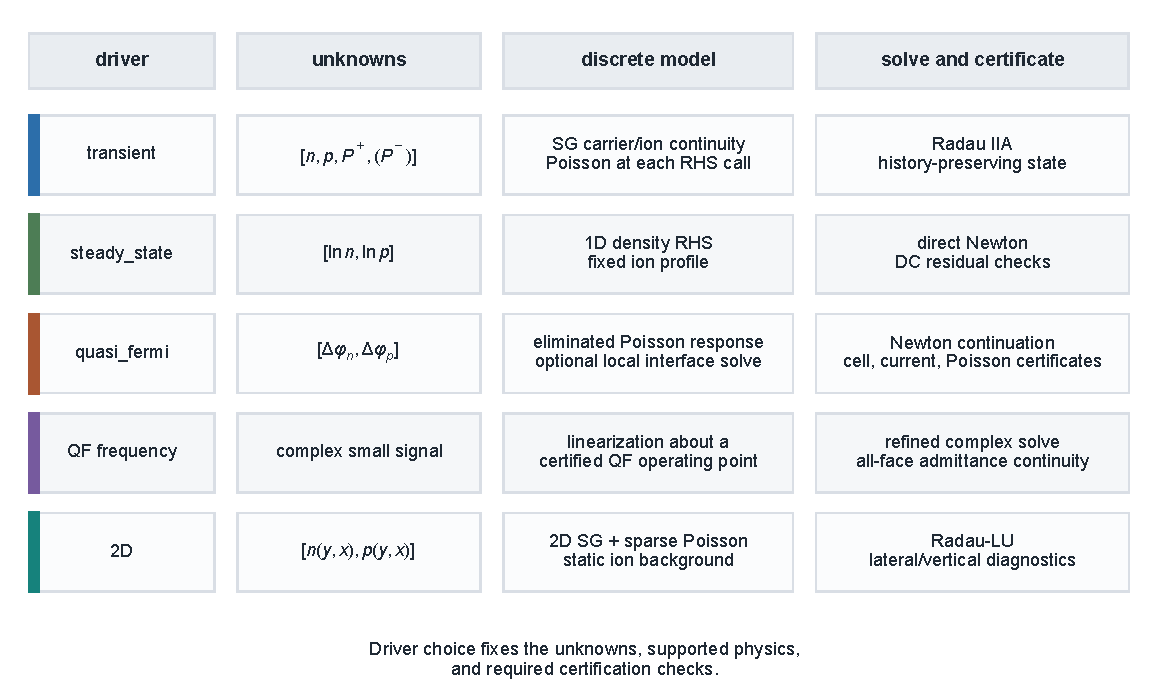
\includegraphics[width=0.98\textwidth,height=\textheight]{figures/solver_topology.pdf}
\caption{Numerical drivers, variable sets, and certification paths}
\end{figure}

The drivers share device construction, grid utilities, Poisson operators
and transport definitions, but they do not solve the same algebraic
problem. The transient driver advances density and configured ion states
in time. The direct steady-state and QF drivers solve different DC
variable sets, while the QF frequency path linearizes about a certified
operating point. The 2D driver uses a separate sparse Poisson operator
and holds the configured ion charge fixed during a J-V run. A J-V point
is reported only after the selected driver has completed its own
relaxation or residual checks.

\hypertarget{spatial-grid}{%
\section{Spatial Grid}\label{spatial-grid}}

The 1D solver builds a multilayer grid over the electrical layers only;
substrate layers are excluded from the electrical grid but retained for
TMM optics. Within each layer of thickness \(L\) the \(N+1\) nodes
follow a hyperbolic-tangent stretching,

\begin{equation}
\label{eq:tanh-grid}
x(\xi)
=
\frac{L}{2}\left[1+\frac{\tanh(a\,\xi)}{\tanh a}\right],
\qquad \xi \in [-1, 1],\ a = 3,
\end{equation}

which clusters nodes toward both layer boundaries. This resolves the
space-charge regions and interface carrier gradients --- where densities
vary over Debye-length scales --- without wasting nodes in the
quasi-neutral interior. Layer grids are concatenated with duplicate
interface points removed, and a compositionally graded layer is
automatically refined by an integer multiplier so a steep band-gap notch
spans several cells.

An optional top-level \texttt{electrical\_grid} block makes the
allocation explicit. Its \texttt{interval\_weights} and \texttt{alphas}
maps are keyed by electrical-layer name and must cover those layers
exactly. Positive interval weights divide the global \texttt{N\_grid}
budget by deterministic largest-remainder allocation, with at least one
interval in each layer and exactly \texttt{N\_grid} intervals overall.
Each positive \texttt{alpha} then sets that layer's tanh clustering
strength. With no block, the historical equal-per-layer grid and grading
multiplier are unchanged. A custom weighted grid cannot be combined with
\texttt{grading\_N\_mult\ \textgreater{}\ 1}, because the two mechanisms
would otherwise compete for the same interval budget.

\hypertarget{method-of-lines-and-state-vector}{%
\section{Method Of Lines And State
Vector}\label{method-of-lines-and-state-vector}}

The PDEs are discretized in space first, producing a coupled system of
ordinary differential equations in time --- the method-of-lines
approach. The packed state vector contains the nodal values

\[
\mathbf{y}=(n,\,p,\,P\,[,P^-]\,[,\mathbf{s}_\mathrm{if}]),
\]

with the optional negative-ion block in dual-ion mode and an optional
trailing block of interface-plane carrier states used by the
steady-state SCAPS-comparison machinery. The electrostatic potential is
\emph{not} a dynamical unknown: Eq. \ref{eq:poisson} is elliptic and is
re-solved exactly, from the instantaneous charge configuration, inside
every right-hand-side (RHS) evaluation. This eliminates any splitting
error between electrostatics and transport at the cost of one linear
solve per evaluation, which the prefactored Poisson path below makes
essentially free.

The exclusive physical interface boundary follows a different
bookkeeping rule. Its four plane densities per interface are solved and
eliminated inside the residual evaluation, so they do not enlarge the
packed device state. This is an algebraic constitutive closure nested
inside the quasi-Fermi solve, not a fast transient appended to the
method-of-lines vector.

\hypertarget{scharfetter-gummel-flux-discretization}{%
\section{Scharfetter-Gummel Flux
Discretization}\label{scharfetter-gummel-flux-discretization}}

Central differencing of the drift-diffusion current (Eq.
\ref{eq:dd-currents}) becomes unstable when the potential drop per cell
exceeds a few \(V_T\) --- the standard failure of naive discretizations
in depletion regions. The Scharfetter-Gummel (SG) scheme instead solves
the constitutive relation \emph{exactly} on each cell under the
assumptions of constant current and constant field between adjacent
nodes; the resulting face flux is the optimal exponential fit,

\begin{equation}
\label{eq:sg-electron}
J_{n,i+1/2}
=
\frac{qD_n}{\Delta x}
\left[
B(\xi)\,n_{i+1}-B(-\xi)\,n_i
\right],
\qquad
\xi = \frac{\phi_{n,i+1}-\phi_{n,i}}{V_T},
\end{equation}

\begin{equation}
\label{eq:sg-hole}
J_{p,i+1/2}
=
\frac{qD_p}{\Delta x}
\left[
B(\xi)\,p_i-B(-\xi)\,p_{i+1}
\right],
\qquad
\xi = \frac{\phi_{p,i+1}-\phi_{p,i}}{V_T},
\end{equation}

with the Bernoulli function

\begin{equation}
\label{eq:bernoulli}
B(\xi)=\frac{\xi}{e^{\xi}-1}.
\end{equation}

The scheme reduces to central differencing in the diffusion limit
(\(|\xi| \ll 1\)) and to pure upwinding in the drift limit
(\(|\xi| \gg 1\)), remaining stable at arbitrarily large cell Peclet
numbers (Scharfetter and Gummel 1969; Selberherr 1984). Its positivity
property is a statement about the \emph{spatial semi-discretization} ---
the face flux is monotone, so the semi-discrete operator does not
manufacture negative densities --- and does not carry over automatically
to the fully discrete transient: the state vector \((n,p,P)\) is
advanced by a general-purpose implicit integrator, which does not
enforce non-negativity at each internal stage or accepted step, and
SolarLab applies no clipping or projection to \(n\) and \(p\) during the
transient. Positivity \emph{is} enforced by construction in the direct
steady-state driver, which solves in logarithmic unknowns (Chapter
\ref{numerical-method}). The scheme rests on three implementation
details:

\begin{itemize}
\tightlist
\item
  the drift argument \(\xi\) is built from the \emph{band-effective}
  potentials \(\phi_n\), \(\phi_p\) of Eqs.
  \ref{eq:band-corrected-potentials}--\ref{eq:dos-potentials}, so
  heterojunction offsets and density-of-states contrasts enter the flux
  without any special-case interface treatment;
\item
  \(B(\xi)\) is evaluated in three numerically safe branches: a Taylor
  series for \(|\xi|<10^{-8}\) (removing the \(0/0\) singularity), the
  analytic zero limit for \(\xi > 700\) (preventing floating-point
  overflow of \(e^{\xi}\)), and the \texttt{expm1} form elsewhere
  (preserving precision near zero);
\item
  face diffusivities use the harmonic mean of the adjacent nodal values,
  the composition consistent with flux continuity across a material
  discontinuity (it also preserves exact zeros, so an ion-blocking layer
  boundary carries strictly zero ionic flux).
\end{itemize}

The divergence of the face fluxes is taken over dual-grid
(finite-volume) cells, so the semi-discrete continuity equations
conserve charge exactly on the non-uniform mesh. The same generalized SG
form discretizes Eq. \ref{eq:ion-flux}, with the electrostatic drop and
the change in excess chemical potential folded into the Bernoulli
argument. The legacy path instead folds the whole-flux factor of Eq.
\ref{eq:ion-flux-legacy} into the face diffusivity.

\hypertarget{poisson-fast-path}{%
\section{Poisson Fast Path}\label{poisson-fast-path}}

The finite-volume Poisson operator is tridiagonal. Its LU factorization
depends only on the grid and the permittivity profile --- both constant
for the lifetime of an experiment --- so it is computed once (LAPACK
\texttt{dgttrf}) and cached; every subsequent RHS evaluation performs a
single \(O(N)\) back-substitution (\texttt{dgttrs}) with the Dirichlet
boundary values absorbed into the right-hand side. This is roughly forty
times faster than a general sparse solve and is the reason the
per-experiment material cache must be built \emph{outside} the time-step
loop.

The same build-once strategy applies to all static coefficient fields:
per-node and per-face material arrays, band-edge and density-of-states
folds, trap-profile lifetime maps, grading profiles, tunnelling-enhanced
Richardson constants, and the TMM generation profile are all assembled
once into an immutable cache. Only three hooks are inherently
state-dependent and re-evaluated per RHS call --- field-dependent
mobility, self-consistent radiative reabsorption, and Robin contact
fluxes --- which is exactly the set excluded from the \texttt{fast}
tier.

\hypertarget{right-hand-side-assembly}{%
\section{Right-Hand-Side Assembly}\label{right-hand-side-assembly}}

Each RHS evaluation proceeds in a fixed order:

\begin{enumerate}
\def\labelenumi{\arabic{enumi}.}
\tightlist
\item
  apply contact conditions to the carrier arrays (ohmic Dirichlet pins,
  or free boundary densities on Robin sides);
\item
  assemble the space charge \(\rho\) (Eq. \ref{eq:charge-density});
\item
  solve Poisson for \(\phi\) via the prefactored path;
\item
  form the generation profile \(G(x)\) (cached TMM or Beer-Lambert; plus
  the reabsorption source when self-consistent photon recycling is
  active);
\item
  recompute face diffusivities from the face field if field-dependent
  mobility is active;
\item
  evaluate SG fluxes, apply the thermionic-emission cap at flagged
  heterointerface faces, and take flux divergences with \(G-R\);
\item
  subtract interface recombination at interface nodes. In the opt-in
  physical QF boundary, locally eliminate the plane states, zero the
  replaced SG face, and insert only the conservative reservoir-to-plane
  drains instead;
\item
  evaluate ion continuity (and the negative species in dual-ion mode);
\item
  enforce the boundary treatment (zero time-derivative on
  Dirichlet-pinned entries; Robin fluxes otherwise), and verify all
  derivatives are finite.
\end{enumerate}

\hypertarget{time-integration-and-robustness}{%
\section{Time Integration And
Robustness}\label{time-integration-and-robustness}}

The semi-discrete system is stiff: electronic relaxation (nanoseconds),
dielectric relaxation, and ionic migration (milliseconds-seconds)
coexist in one state vector. SolarLab integrates it with SciPy's Radau
IIA method --- a fifth-order, L-stable, fully implicit Runge-Kutta
scheme appropriate for stiff differential systems (Hairer and Wanner
1996) --- with BDF as a fallback. Stability of the implicit iteration,
not accuracy, sets the practical step size, and a layered set of
safeguards keeps difficult J-V steps bounded:

\begin{itemize}
\tightlist
\item
  \textbf{Step-size ceiling near flat band.} Close to
  \(V_\mathrm{app} \approx |V_\mathrm{bi}|\) the Jacobian is nearly
  singular and Radau's local-error estimator can under-report the
  truncation error, accepting a single oversized step onto a spurious
  branch of the implicit equations (visible as an isolated non-physical
  J-V spike). Every voltage step therefore caps the internal step at
  \(1/20\) of the settle interval.
\item
  \textbf{Evaluation budget.} A per-step ceiling on RHS evaluations
  converts a non-contracting implicit iteration (which would otherwise
  spin without wall-time bound) into a recoverable failure.
\item
  \textbf{Bisection in time.} A failed settle interval is halved and
  re-chained, up to \(2^{10}\) sub-intervals.
\item
  \textbf{Frozen-source retry.} The self-consistent reabsorption source
  couples all absorber nodes through a non-local integral; at the
  diode-injection knee this can prevent Newton contraction inside Radau.
  The failed step is retried with the reabsorption source frozen at its
  entry-state value --- a lag bounded by one settle interval, well below
  the regression tolerance.
\item
  \textbf{Method fallback.} A step that exhausts bisection is attempted
  once with BDF, which occasionally converges where Radau's error
  estimator stalls.
\item
  \textbf{Finite-value guard.} Any NaN/Inf in the assembled derivatives
  raises immediately rather than letting the integrator accept corrupted
  state.
\end{itemize}

\hypertarget{direct-steady-state-solver}{%
\section{Direct Steady-State Solver}\label{direct-steady-state-solver}}

The transient integrator is the reference engine for ion-coupled
dynamics, but steady-state comparisons (e.g.~against ion-free
steady-state simulators such as SCAPS) and artifact-free open-circuit
voltages benefit from solving \(F(\mathbf{y}) = 0\) directly on the
\emph{same} discretized RHS --- one physics implementation, two drivers.
The steady-state driver freezes the ion profile from its seed state and
applies a damped Newton method with:

\begin{itemize}
\tightlist
\item
  \textbf{Logarithmic unknowns} \(z = (\ln n, \ln p)\), which enforce
  positivity by construction and equidistribute sensitivity across
  densities spanning twenty orders of magnitude;
\item
  \textbf{Peak-density residual scaling}: residuals are normalized by
  the global peak density rather than the local one, because at dark
  depletion nodes the local-relative rate floors at double-precision
  cancellation noise and no tolerance could ever be met; on the
  peak-density scale that noise sits near \(10^{-10}\) while a physical
  imbalance registers at order unity, and the tolerance translates into
  a terminal-current error bound of \(\sim 10^{-8}\,A\,m^{-2}\);
\item
  \textbf{Finite-difference Jacobian with chord reuse}: the dense
  Jacobian is built by forward differences and its LU factorization is
  reused across chord iterations, rebuilt only when a stale factor loses
  contraction --- the dominant cost saving on warm-started continuation
  solves;
\item
  \textbf{Backtracking line search} on the residual 2-norm, with the
  Newton step capped in log space;
\item
  \textbf{Smoothed thermionic-emission cap}: the hard magnitude-minimum
  of the TE cap is non-differentiable exactly where it binds; the
  steady-state driver (and only it) replaces it with a narrow sigmoid
  blend so Newton retains a usable derivative;
\item
  \textbf{Quasi-Fermi-preserving Poisson relaxation}: before Newton
  starts (and after every transient assist), a nonlinear Poisson solve
  with Boltzmann-responding carriers at frozen quasi-Fermi levels
  performs the dielectric relaxation analytically. This step is
  unconditionally well-posed and removes the seconds-slow relaxation
  mode that otherwise dominates the Jacobian conditioning in
  near-insulating layers;
\item
  \textbf{Certified fallbacks}: where the TE-cap kink makes Newton stall
  at an already-physically-converged state, the best iterate is accepted
  under an explicit residual bound; where Newton cannot finish at all,
  escalating Radau settles compute the point and are \emph{certified}
  against the same residual scale; an uncertifiable point raises an
  error rather than returning an unconverged result.
\end{itemize}

Steady-state J-V curves are computed by voltage continuation with
warm-started seeds and automatic voltage-step bisection; the
open-circuit voltage can additionally be located by direct bisection on
the steady-state \(J(V)\) zero crossing, eliminating sweep-grid
interpolation error. Measured agreement between the two drivers on the
reference configuration is within 5 mV in \(V_\mathrm{oc}\) and 1\% in
\(J_\mathrm{sc}\). Two deep-tail regimes are handled by the transient
engine rather than the Newton driver: near-insulating contact doping
produces no \(J = 0\) crossing below the scan ceiling (a physical
absence the transient confirms), and deeply collapsed
conduction-band-offset junctions are pathological for any algebraic
Newton method and are handled by the transient engine only.

\hypertarget{cancellation-safe-quasi-fermi-steady-state}{%
\section{Cancellation-Safe Quasi-Fermi Steady
State}\label{cancellation-safe-quasi-fermi-steady-state}}

The \texttt{quasi\_fermi} driver targets steady states in which the
terminal current is the small difference between very large forward and
reverse SG terms. This is the relevant numerical regime in a highly
doped crystalline-silicon emitter and in the zero-thickness interface
closure. Reaching a small algebraic residual in density variables is not
enough there: direct subtraction can lose the current before Newton sees
it.

SolarLab instead solves for increments of the electron and hole
quasi-Fermi potentials,

\begin{equation}
\label{eq:qf-potentials}
\varphi_n=V_T\ln n-(\phi+\chi),\qquad
\varphi_p=V_T\ln p+(\phi+\chi+E_g).
\end{equation}

A transport-balanced reference state is retained separately from the
Newton increments. Poisson and the Boltzmann carrier response are
eliminated to tight tolerance at every residual evaluation. For a face
whose two exponential SG legs are \(a\) and \(b\), the current is
evaluated from the known quasi-Fermi drop \(\delta\) using

\[
a-b=
\begin{cases}
-a\,\operatorname{expm1}(-\delta), & \delta\geq0,\\
b\,\operatorname{expm1}(\delta), & \delta<0,
\end{cases}
\]

rather than by subtracting the two rounded absolute legs. Reference and
increment drops are never collapsed into one absolute potential and then
differenced again.

Illuminated states are reached by source continuation from dark
equilibrium. The Newton termination test is only a numerical stopping
condition. A point is returned only when independent gates also pass for
the normalized cell residual, the integrated electron and hole
continuity defects, the peak-to-peak all-face current spread, and the
Poisson residual. The physical interface path adds the local
plane-closure residual to that certificate.

For the physical interface boundary, the final Newton stage uses
face-drop coordinates rather than nodal quasi-Fermi values. For each
carrier the closing drop is formed as

\[
d_{\mathrm{last}}=-\sum_{i<\mathrm{last}}d_i,
\]

which pins both contact increments exactly while retaining sub-ULP
interior drops. A certified state transferred to another mesh is
regridded by conservative overlap of these face drops, with the
round-off remainder placed on the closing face. A nodal-coordinate solve
may be used to locate the basin, but the target mesh is always re-solved
and re-certified in face-drop coordinates before it is reported.

This driver is intentionally narrower than the transient engine. It
currently supports illuminated, local, ion-free J-V with ideal carrier
pins and local recombination. Mobile or background ions, selective
contacts, field-dependent mobility, non-local photon recycling, the
older dynamic interface-state block, and thermionic/cross-node interface
terms outside the exclusive boundary are rejected. A stack marked
\texttt{jv\_solver\_policy:\ cancellation\_safe\_qf\_required} cannot
run a production J-V through another variable set; an explicit
diagnostic override is labelled unvalidated rather than being treated as
equivalent physics.

\hypertarget{operator-splitting-for-slow-ion-dynamics}{%
\section{Operator Splitting For Slow Ion
Dynamics}\label{operator-splitting-for-slow-ion-dynamics}}

Long-time experiments (degradation) use an operator-splitting step
matched to the two-time-scale structure: the ion subsystem is advanced
over a macroscopic interval with the carrier densities frozen (Poisson
re-solved inside the ion RHS, so the ions always see a field consistent
with the \emph{current ion profile and the frozen carriers}), and the
carriers are then re-equilibrated by a short full-system transient of
order one carrier lifetime. Re-solving Poisson makes the potential
consistent with the instantaneous charge density; it does not keep the
electrons and holes quasi-stationary with respect to the evolving ionic
field, so this is a first-order operator splitting rather than a fully
self-consistent electron-ion advance. Its error grows with the
macro-step and with the band-bending change the ions produce over that
step, so a macro-step halving study against the fully coupled solution
is the appropriate check before quoting long-time results --- most
importantly near open circuit and near flat band, where the ionic
screening moves the bands the furthest. Snapshot J-V measurements inside
degradation freeze the ion profile entirely, so each snapshot reports
the instantaneous electronic response of the current ionic
configuration.

\hypertarget{terminal-current-evaluation}{%
\section{Terminal Current
Evaluation}\label{terminal-current-evaluation}}

The reported current density combines conduction, ionic, and
displacement contributions at mesh faces:

\[
J = J_n + J_p + J_\mathrm{ion} + \varepsilon_0\varepsilon_r
\frac{\partial E}{\partial t}.
\]

Transient sweeps read the contact-adjacent face, where the displacement
term is part of the physical external-circuit current. Steady-state
probes (Suns-\(V_\mathrm{oc}\), EQE) instead take the \emph{median}
across interior faces: charge conservation makes \(J(x)\) uniform at
steady state, so any face is formally correct, but residual ionic and
displacement transients concentrate at the boundary faces and the median
is robust to those outliers.

Because a median summarises the face-to-face disagreement rather than
removing it, both steady-state probes also report how large that
disagreement was,

\[
\Delta J_\mathrm{spread}=\max_x J(x)-\min_x J(x),
\]

evaluated over the interior faces only --- the two contact-adjacent
faces are excluded because their displacement term is physical
external-circuit current and legitimately swings on ionic-rich stacks,
so including them would report a real boundary transient as a
conservation error. The value is returned as \texttt{J\_spread\_max} on
both result objects.

SolarLab reports this value but does not use it as an acceptance test.
Although \(J(x)\) is uniform at an exact steady state, the raw transient
endpoint does not support a fixed \(\Delta J_\mathrm{spread}\) threshold
for \(V_\mathrm{oc}\), \(J_\mathrm{sc}\) or FF. On the TMM presets, the
median current is already stable while the spread remains non-monotone
in settling time and strongly mesh-dependent.

At the raw endpoint, the anomalous spread is dominated by the local
error of Radau's final unbounded step: \texttt{run\_transient} is called
with \texttt{max\_step=inf} and \texttt{t\_eval={[}t\_end{]}}, so near a
fixed point the controller can inflate its last step to the scale of the
full settling interval. Re-entering the integrator for one short
controlled leg reduced the interior spread by about 390x on
\texttt{nip\_MAPbI3} and 39,700x on \texttt{ionmonger\_benchmark}, while
moving the median by no more than \(2.4\times10^{-4}\,A\,m^{-2}\). The
terminal electron, hole, ionic and displacement components do not show a
cancellation large enough to explain that raw endpoint anomaly. After
the controlled leg, any remaining conduction-current spread is paired
with the displacement term and can represent a genuinely unequilibrated
ionic state.

Use the raw spread as a diagnostic, not as a fixed pass/fail threshold
for the photovoltaic metrics. A longer nominal settling interval does
not necessarily remove the final-step error. Control the final step,
then refine the mesh until the \emph{extracted metrics} stop moving.
Metrics extraction interpolates \(J_\mathrm{sc}\) at \(V=0\). For
\(J_\mathrm{sc}\ne0\), it brackets \(V_\mathrm{oc}\) at the first pair
satisfying \(J_i>J_\mathrm{tol}\) and \(J_{i+1}\le J_\mathrm{tol}\),
where \(J_\mathrm{tol}=10^{-3}|J_\mathrm{sc}|\); a genuine sign crossing
is the common case, while a collapsed-current curve may reach this
declared resolution floor without changing sign. FF and PCE are then
computed over the resolved operating quadrant. The
\texttt{voc\_bracketed} flag reports whether this metric bracket was
found and accepted, not whether a literal positive-to-negative sign
change occurred. The hysteresis index compares scan directions as

\[
\mathrm{HI}
=
\frac{PCE_\mathrm{rev}-PCE_\mathrm{fwd}}{PCE_\mathrm{rev}} .
\]

\hypertarget{two-dimensional-extension}{%
\section{Two-Dimensional Extension}\label{two-dimensional-extension}}

The experimental 2D solver reuses the same physics on a tensor-product
grid: the tanh-clustered stack axis crossed with a uniform lateral axis.
The 2D Poisson operator is a five-point finite-volume stencil with
harmonic-mean face permittivities, factorized once with a sparse LU and
reused per evaluation; the carrier fluxes are vectorized 2D SG forms
with the same band-effective potentials, and the thermionic-emission cap
applies on vertical (stack-direction) heterointerface faces. Mobile ions
are held as a static Poisson background extruded from the 1D solution
--- the documented 2D model assumption. Lateral boundaries are periodic
or zero-flux. The 2D solver is regression-gated against 1D in the
lateral-uniform limit to \(|\Delta V_\mathrm{oc}| \leq 0.1\) mV,
relative \(\Delta J_\mathrm{sc} \leq 5\times10^{-4}\), and
\(|\Delta FF| \leq 10^{-3}\).

\hypertarget{numerical-safety}{%
\section{Numerical Safety}\label{numerical-safety}}

Important safety mechanisms include:

\begin{itemize}
\tightlist
\item
  finite-value guards in the RHS;
\item
  harmonic face permittivity;
\item
  stable Bernoulli-function branches;
\item
  the thermionic-emission cap at abrupt heterointerfaces;
\item
  step-size ceilings, evaluation budgets, and bisection/fallback logic
  in every voltage-stepping experiment;
\item
  TMM determinant guard;
\item
  median-current steady-state readout;
\item
  explicit \texttt{voc\_bracketed} flags when a J-V sweep does not
  resolve an accepted open-circuit bracket;
\item
  steady-state convergence raises on non-convergence.
\end{itemize}

For publication work, numerical settings are part of the method. Report
the grid size, voltage spacing, settling time or scan rate, tolerances
when modified, and whether the run used \texttt{legacy}, \texttt{fast},
or \texttt{full} mode.

\hypertarget{running-solarlab}{%
\chapter{Running SolarLab}\label{running-solarlab}}

\hypertarget{installation}{%
\section{Installation}\label{installation}}

From \texttt{perovskite-sim/}:

\begin{Shaded}
\begin{Highlighting}[]
\ExtensionTok{pip}\NormalTok{ install }\AttributeTok{{-}e} \StringTok{".[dev]"}
\end{Highlighting}
\end{Shaded}

For the frontend:

\begin{Shaded}
\begin{Highlighting}[]
\BuiltInTok{cd}\NormalTok{ frontend}
\ExtensionTok{npm}\NormalTok{ install}
\end{Highlighting}
\end{Shaded}

\hypertarget{backend}{%
\section{Backend}\label{backend}}

From the SolarLab root:

\begin{Shaded}
\begin{Highlighting}[]
\ExtensionTok{uvicorn}\NormalTok{ backend.main:app }\DataTypeTok{\textbackslash{}}
  \AttributeTok{{-}{-}host}\NormalTok{ 127.0.0.1 }\AttributeTok{{-}{-}port}\NormalTok{ 8000 }\DataTypeTok{\textbackslash{}}
  \AttributeTok{{-}{-}app{-}dir}\NormalTok{ perovskite{-}sim }\AttributeTok{{-}{-}reload}
\end{Highlighting}
\end{Shaded}

Do not run \texttt{uvicorn\ main:app} from inside \texttt{backend/}; the
backend imports are written around \texttt{-\/-app-dir\ perovskite-sim}.

\hypertarget{frontend}{%
\section{Frontend}\label{frontend}}

\begin{Shaded}
\begin{Highlighting}[]
\BuiltInTok{cd}\NormalTok{ perovskite{-}sim/frontend}
\ExtensionTok{npm}\NormalTok{ run dev}
\end{Highlighting}
\end{Shaded}

Then open:

\begin{verbatim}
http://127.0.0.1:5173
\end{verbatim}

\hypertarget{python-api}{%
\section{Python API}\label{python-api}}

\begin{Shaded}
\begin{Highlighting}[]
\ImportTok{from}\NormalTok{ perovskite\_sim.models.config\_loader }\ImportTok{import}\NormalTok{ load\_device\_from\_yaml}
\ImportTok{from}\NormalTok{ perovskite\_sim.experiments.jv\_sweep }\ImportTok{import}\NormalTok{ run\_jv\_sweep}

\NormalTok{stack }\OperatorTok{=}\NormalTok{ load\_device\_from\_yaml(}\StringTok{"configs/nip\_MAPbI3.yaml"}\NormalTok{)}
\NormalTok{result }\OperatorTok{=}\NormalTok{ run\_jv\_sweep(stack, N\_grid}\OperatorTok{=}\DecValTok{80}\NormalTok{, n\_points}\OperatorTok{=}\DecValTok{40}\NormalTok{, v\_rate}\OperatorTok{=}\FloatTok{1.0}\NormalTok{)}

\BuiltInTok{print}\NormalTok{(result.metrics\_fwd.V\_oc)}
\BuiltInTok{print}\NormalTok{(result.metrics\_fwd.J\_sc)}
\BuiltInTok{print}\NormalTok{(result.metrics\_fwd.FF)}
\BuiltInTok{print}\NormalTok{(result.metrics\_fwd.PCE)}
\end{Highlighting}
\end{Shaded}

\hypertarget{worked-example-1-baseline-j-v-sweep}{%
\section{Worked Example 1: Baseline J-V
Sweep}\label{worked-example-1-baseline-j-v-sweep}}

This example runs a standard n-i-p MAPbI3 J-V sweep and reports the
principal photovoltaic metrics.

\begin{Shaded}
\begin{Highlighting}[]
\BuiltInTok{cd}\NormalTok{ perovskite{-}sim}
\ExtensionTok{python} \AttributeTok{{-}} \OperatorTok{\textless{}\textless{}\textquotesingle{}PY\textquotesingle{}}
\StringTok{from perovskite\_sim.models.config\_loader import load\_device\_from\_yaml}
\StringTok{from perovskite\_sim.experiments.jv\_sweep import run\_jv\_sweep}

\StringTok{stack = load\_device\_from\_yaml("configs/nip\_MAPbI3.yaml")}
\StringTok{result = run\_jv\_sweep(stack, N\_grid=80, n\_points=40, v\_rate=1.0)}
\StringTok{m = result.metrics\_fwd}
\StringTok{print(f"Voc = \{m.V\_oc:.4f\} V")}
\StringTok{print(f"Jsc = \{m.J\_sc:.2f\} A/m\^{}2")}
\StringTok{print(f"FF  = \{m.FF:.3f\}")}
\StringTok{print(f"PCE = \{100*m.PCE:.2f\} \%")}
\StringTok{print(f"Voc bracketed: \{m.voc\_bracketed\}")}
\OperatorTok{PY}
\end{Highlighting}
\end{Shaded}

Metric interpretation:

\begin{itemize}
\tightlist
\item
  \(J_\mathrm{sc}\) is the current density near zero applied voltage.
\item
  \(V_\mathrm{oc}\) is extracted from the first current-resolution
  bracket, \(J_\mathrm{tol}=10^{-3}|J_\mathrm{sc}|\); on an ordinary
  curve this is the neighborhood of the terminal-current zero crossing.
  The bracket must also pass the configured thermodynamic voltage
  ceiling.
\item
  FF and PCE are meaningful only when \texttt{voc\_bracketed} is true.
\item
  Forward and reverse metrics can differ when mobile ions retain scan
  history.
\end{itemize}

\hypertarget{worked-example-2-absorber-thickness-study}{%
\section{Worked Example 2: Absorber Thickness
Study}\label{worked-example-2-absorber-thickness-study}}

This example varies absorber thickness while leaving the rest of the
stack unchanged, allowing optical collection and recombination trends to
be compared under controlled assumptions.

\begin{Shaded}
\begin{Highlighting}[]
\ImportTok{from}\NormalTok{ dataclasses }\ImportTok{import}\NormalTok{ replace}
\ImportTok{from}\NormalTok{ perovskite\_sim.models.config\_loader }\ImportTok{import}\NormalTok{ load\_device\_from\_yaml}
\ImportTok{from}\NormalTok{ perovskite\_sim.experiments.jv\_sweep }\ImportTok{import}\NormalTok{ run\_jv\_sweep}

\NormalTok{base }\OperatorTok{=}\NormalTok{ load\_device\_from\_yaml(}\StringTok{"configs/nip\_MAPbI3.yaml"}\NormalTok{)}
\NormalTok{absorber\_index }\OperatorTok{=} \BuiltInTok{next}\NormalTok{(i }\ControlFlowTok{for}\NormalTok{ i, layer }\KeywordTok{in} \BuiltInTok{enumerate}\NormalTok{(base.layers)}
                      \ControlFlowTok{if}\NormalTok{ layer.role }\OperatorTok{==} \StringTok{"absorber"}\NormalTok{)}

\ControlFlowTok{for}\NormalTok{ thickness\_nm }\KeywordTok{in}\NormalTok{ (}\DecValTok{200}\NormalTok{, }\DecValTok{400}\NormalTok{, }\DecValTok{700}\NormalTok{, }\DecValTok{1000}\NormalTok{):}
\NormalTok{    layers }\OperatorTok{=} \BuiltInTok{list}\NormalTok{(base.layers)}
\NormalTok{    layers[absorber\_index] }\OperatorTok{=}\NormalTok{ replace(}
\NormalTok{        layers[absorber\_index],}
\NormalTok{        thickness}\OperatorTok{=}\NormalTok{thickness\_nm }\OperatorTok{*} \FloatTok{1e{-}9}\NormalTok{,}
\NormalTok{    )}
\NormalTok{    stack }\OperatorTok{=}\NormalTok{ replace(base, layers}\OperatorTok{=}\BuiltInTok{tuple}\NormalTok{(layers))}
\NormalTok{    result }\OperatorTok{=}\NormalTok{ run\_jv\_sweep(stack, N\_grid}\OperatorTok{=}\DecValTok{80}\NormalTok{, n\_points}\OperatorTok{=}\DecValTok{30}\NormalTok{, v\_rate}\OperatorTok{=}\FloatTok{2.0}\NormalTok{)}
\NormalTok{    m }\OperatorTok{=}\NormalTok{ result.metrics\_fwd}
    \BuiltInTok{print}\NormalTok{(thickness\_nm, m.V\_oc, m.J\_sc, m.FF, m.PCE)}
\end{Highlighting}
\end{Shaded}

Expected interpretation:

\begin{itemize}
\tightlist
\item
  Thicker absorbers can absorb more light, but can also increase
  recombination or transport loss.
\item
  If \(J_\mathrm{sc}\) does not change under Beer-Lambert optics, check
  whether \texttt{alpha} and \texttt{Phi} are physically configured.
\item
  If FF collapses, inspect spatial profiles and contact selectivity
  before concluding that the absorber is intrinsically poor.
\end{itemize}

\hypertarget{worked-example-3-enabling-tmm-optics}{%
\section{Worked Example 3: Enabling TMM
Optics}\label{worked-example-3-enabling-tmm-optics}}

This example compares scalar Beer-Lambert generation with
wavelength-resolved transfer-matrix generation.

\begin{Shaded}
\begin{Highlighting}[]
\ImportTok{from}\NormalTok{ perovskite\_sim.models.config\_loader }\ImportTok{import}\NormalTok{ load\_device\_from\_yaml}
\ImportTok{from}\NormalTok{ perovskite\_sim.experiments.jv\_sweep }\ImportTok{import}\NormalTok{ run\_jv\_sweep}

\ControlFlowTok{for}\NormalTok{ config }\KeywordTok{in}\NormalTok{ (}\StringTok{"configs/nip\_MAPbI3.yaml"}\NormalTok{, }\StringTok{"configs/nip\_MAPbI3\_tmm.yaml"}\NormalTok{):}
\NormalTok{    stack }\OperatorTok{=}\NormalTok{ load\_device\_from\_yaml(config)}
\NormalTok{    result }\OperatorTok{=}\NormalTok{ run\_jv\_sweep(stack, N\_grid}\OperatorTok{=}\DecValTok{60}\NormalTok{, n\_points}\OperatorTok{=}\DecValTok{21}\NormalTok{)}
    \BuiltInTok{print}\NormalTok{(config, result.metrics\_fwd.J\_sc)}
\end{Highlighting}
\end{Shaded}

Expected interpretation:

\begin{itemize}
\tightlist
\item
  TMM includes interference, reflection, parasitic absorption, and
  spectral weighting.
\item
  TMM results are only as credible as the \texttt{optical\_material}
  data and AM1.5G spectrum used.
\item
  EQE and EL should use TMM-enabled configurations, not
  Beer-Lambert-only presets.
\end{itemize}

\hypertarget{backend-api}{%
\chapter{Backend API}\label{backend-api}}

Configuration endpoints:

\begin{longtable}[]{@{}lll@{}}
\toprule
Method & Path & Purpose \\
\midrule
\endhead
\texttt{GET} & \texttt{/api/configs} & list shipped and user presets \\
\texttt{GET} & \texttt{/api/configs/\{name\}} & load one preset \\
\texttt{POST} & \texttt{/api/configs/user} & save a user-edited stack \\
\texttt{GET} & \texttt{/api/layer-templates} & layer template library \\
\texttt{GET} & \texttt{/api/optical-materials} & available TMM optical
keys \\
\bottomrule
\end{longtable}

Preferred experiment interface:

\begin{longtable}[]{@{}lll@{}}
\toprule
Method & Path & Purpose \\
\midrule
\endhead
\texttt{POST} & \texttt{/api/jobs} & submit
\texttt{\{kind,\ config\_path\textbar{}device,\ params\}} \\
\texttt{GET} & \texttt{/api/jobs/\{id\}/events} & stream
progress/result/error/done events \\
\bottomrule
\end{longtable}

When the backend is running, \texttt{/docs} shows the interactive
FastAPI schema and \texttt{/openapi.json} provides the machine-readable
version. The streaming job endpoint accepts four top-level fields:

\begin{longtable}[]{@{}
  >{\raggedright\arraybackslash}p{(\columnwidth - 2\tabcolsep) * \real{0.50}}
  >{\raggedright\arraybackslash}p{(\columnwidth - 2\tabcolsep) * \real{0.50}}@{}}
\toprule
Field & Use \\
\midrule
\endhead
\texttt{kind} & required experiment name \\
\texttt{config\_path} & preset path or name; required unless an inline
\texttt{device} is supplied \\
\texttt{device} & inline device object; takes precedence over
\texttt{config\_path} for single-stack jobs \\
\texttt{params} & job-specific settings; defaults to an empty object \\
\bottomrule
\end{longtable}

The \texttt{tandem} job is the exception: it requires
\texttt{config\_path} because its YAML contains more than one subcell. A
typical J-V submission is:

\begin{Shaded}
\begin{Highlighting}[]
\FunctionTok{\{}
  \DataTypeTok{"kind"}\FunctionTok{:} \StringTok{"jv"}\FunctionTok{,}
  \DataTypeTok{"config\_path"}\FunctionTok{:} \StringTok{"configs/cSi\_homojunction.yaml"}\FunctionTok{,}
  \DataTypeTok{"params"}\FunctionTok{:} \FunctionTok{\{}
    \DataTypeTok{"solver"}\FunctionTok{:} \StringTok{"quasi\_fermi"}\FunctionTok{,}
    \DataTypeTok{"N\_grid"}\FunctionTok{:} \DecValTok{200}\FunctionTok{,}
    \DataTypeTok{"n\_points"}\FunctionTok{:} \DecValTok{42}\FunctionTok{,}
    \DataTypeTok{"V\_max"}\FunctionTok{:} \FloatTok{0.7}
  \FunctionTok{\}}
\FunctionTok{\}}
\end{Highlighting}
\end{Shaded}

Submission returns \texttt{\{"status":"ok","job\_id":"..."\}}. The
client then opens the event stream for that ID:

\begin{longtable}[]{@{}ll@{}}
\toprule
SSE event & Payload \\
\midrule
\endhead
\texttt{progress} & \texttt{stage}, \texttt{current}, \texttt{total},
\texttt{eta\_s}, and \texttt{message} \\
\texttt{result} & final serialized experiment result \\
\texttt{error} & \texttt{message} describing a worker failure \\
\texttt{done} & empty terminal marker, emitted after either result or
error \\
\bottomrule
\end{longtable}

For \texttt{kind="jv"}, the streaming defaults and compatibility rules
are:

\begingroup\footnotesize\setlength{\tabcolsep}{3.5pt}

\renewcommand{\arraystretch}{1.18}
\begin{longtable}{@{}>{\raggedright\arraybackslash}p{0.38\linewidth}>{\raggedright\arraybackslash}p{0.27\linewidth}>{\raggedright\arraybackslash}p{0.27\linewidth}@{}}
\toprule
Parameter & Job default & Use \\
\midrule
\endhead
\path{N_grid} & 60 & global electrical-grid budget \\
\path{n_points} & 30 & requested voltage samples \\
\path{v_rate} & 1.0 & transient scan rate; ignored by zero-scan-rate drivers \\
\path{V_max} & driver default & upper requested bias \\
\path{illuminated} & true & \path{quasi_fermi} currently rejects dark J-V \\
\path{solver} & \path{transient} & \path{transient}, \path{steady_state}, or \path{quasi_fermi} \\
\path{iface_states} & false & older plane-state option for \path{steady_state} only \\
\path{interface_boundary} & false & exclusive physical boundary; requires \path{quasi_fermi} \\
\path{interface_transport_model} & \path{fermi_richardson} & meaningful only with the physical boundary enabled \\
\bottomrule
\end{longtable}
\endgroup

The synchronous \texttt{/api/jv} compatibility route accepts the same
named J-V fields but defaults to \texttt{N\_grid=80} and
\texttt{n\_points=40}. Because \texttt{/api/jobs.params} is a generic
object, OpenAPI cannot validate every job-specific key before dispatch.
Unknown or unused parameters may be ignored; use the table for the
selected job and confirm the serialized settings in reproducibility
work.

Supported job kinds:

\begin{verbatim}
jv, current_decomp, spatial, dark_jv, suns_voc, voc_t,
eqe, el, impedance, tpv, degradation, tandem,
mott_schottky, jv_2d, voc_grain_sweep
\end{verbatim}

The frontend primarily uses streaming jobs. Long-running experiments
report progress through callbacks that the backend converts to SSE
frames.

\hypertarget{experiment-manual}{%
\chapter{Experiment Manual}\label{experiment-manual}}

\hypertarget{j-v-sweep}{%
\section{J-V Sweep}\label{j-v-sweep}}

The J-V sweep runs forward and reverse voltage scans while preserving
state history. This state-preserving scan is the implemented
representation of hysteresis in an ion-coupled perovskite cell.

Outputs:

\begin{itemize}
\tightlist
\item
  \texttt{V\_fwd}, \texttt{J\_fwd};
\item
  \texttt{V\_rev}, \texttt{J\_rev};
\item
  \texttt{metrics\_fwd}, \texttt{metrics\_rev};
\item
  \texttt{hysteresis\_index}.
\end{itemize}

Metrics:

\[
FF=\frac{P_\mathrm{mpp}}{V_\mathrm{oc}J_\mathrm{sc}}.
\]

\[
PCE=\frac{P_\mathrm{mpp}}{P_\mathrm{in}},
\qquad
P_\mathrm{in} = 1000\,W\,m^{-2}\ \text{by default (AM1.5G, 1 sun)}.
\]

The low-level metric extractor accepts an explicit \texttt{P\_in}. The
Python QF J-V driver exposes it as \texttt{P\_in\_W\_m2}; the current
transient and density-Newton drivers, and all backend J-V routes, do not
yet forward it. For those paths, a run that changes illumination
intensity or spectrum must recompute the branch metrics from the
returned arrays:

\begin{Shaded}
\begin{Highlighting}[]
\ImportTok{from}\NormalTok{ perovskite\_sim.experiments.jv\_sweep }\ImportTok{import}\NormalTok{ compute\_metrics}

\NormalTok{m }\OperatorTok{=}\NormalTok{ compute\_metrics(result.V\_fwd, result.J\_fwd, P\_in}\OperatorTok{=}\NormalTok{actual\_power\_W\_m2)}
\end{Highlighting}
\end{Shaded}

Until that recomputation is made, \texttt{result.metrics\_fwd.PCE} and
\texttt{result.metrics\_rev.PCE} retain the 1-sun denominator of
\(1000\,W\,m^{-2}\). The denominator is fixed by the current driver
interface; the optical model does not impose it.

If the sweep never reaches the current-resolution bracket,
\texttt{voc\_bracketed=false}. The same flag is returned when an
extracted voltage is rejected by the configured thermodynamic ceiling.
In either case \(V_\mathrm{oc}\), FF, and PCE are sentinel values;
inspect the voltage range, band-gap ceiling and point-status records
before deciding whether to increase \texttt{V\_max}.

The J-V job additionally accepts a solver selector: the default
\texttt{transient} driver is the state-preserving Radau sweep described
above, while \texttt{steady\_state} routes the same device through the
ion-frozen direct Newton driver of Chapter \ref{numerical-method},
returning a single hysteresis-free steady-state curve. The steady-state
driver is the appropriate choice when comparing against ion-free
steady-state simulators.

\texttt{quasi\_fermi} selects the cancellation-safe, certificate-bearing
driver. It currently returns an illuminated zero-scan-rate curve only,
represented in the common result schema with identical forward and
reverse branches and zero hysteresis. \texttt{interface\_boundary=true}
is accepted only with this driver and activates the exclusive
zero-thickness physical boundary described in Eq.
\ref{eq:physical-interface-qss}. Its
\texttt{interface\_transport\_model} is one of
\texttt{fermi\_richardson}, \texttt{scaps\_thermionic}, or
\texttt{scaps\_thermal\_velocity}; choosing a non-default model while
the boundary is off is rejected. Dark J-V and ion-history studies remain
on the transient path.

The solver choice is not a convenience fallback. A stack whose
\texttt{jv\_solver\_policy} requires cancellation-safe quasi-Fermi
variables rejects the transient and density-Newton drivers for
production use. Conversely, a QF request containing unsupported physics
raises an error instead of dropping that physics or silently routing to
another solver. Per-point QF status records carry the continuity,
current-spread, Poisson, and normalized-residual certificates used to
accept the curve.

\hypertarget{current-decomposition}{%
\section{Current Decomposition}\label{current-decomposition}}

Current decomposition separates:

\begin{itemize}
\tightlist
\item
  electron current \(J_n\);
\item
  hole current \(J_p\);
\item
  ion current \(J_\mathrm{ion}\);
\item
  displacement current \(J_\mathrm{disp}\);
\item
  total current.
\end{itemize}

This separation helps identify whether a transient is dominated by
electronic, ionic, or capacitive response.

\hypertarget{spatial-profiles}{%
\section{Spatial Profiles}\label{spatial-profiles}}

Spatial-profile runs save snapshots of:

\begin{itemize}
\tightlist
\item
  \(x\);
\item
  \(\phi\);
\item
  \(E\);
\item
  \(n\);
\item
  \(p\);
\item
  \(P\);
\item
  \(\rho\);
\item
  applied voltage.
\end{itemize}

These profiles are essential for interpreting unusual J-V behavior. For
example, a high \(V_\mathrm{oc}\) with poor FF may indicate
selective-contact or recombination issues rather than poor optical
generation.

\hypertarget{dark-j-v}{%
\section{Dark J-V}\label{dark-j-v}}

Dark J-V fits the diode equation:

\[
J=J_0\left[\exp\left(\frac{V}{n_\mathrm{id}V_T}\right)-1\right].
\]

The output includes ideality factor \(n_\mathrm{id}\), saturation
current \(J_0\), and the fitted voltage window.

\hypertarget{suns-v_mathrmoc}{%
\section{\texorpdfstring{Suns-\(V_\mathrm{oc}\)}{Suns-V\_\textbackslash mathrm\{oc\}}}\label{suns-v_mathrmoc}}

Suns-\(V_\mathrm{oc}\) varies illumination intensity and extracts
\(V_\mathrm{oc}\) at each level. It constructs a pseudo-JV curve:

\[
J_\mathrm{pseudo}(X)
=J_{\mathrm{sc,ref}}-J_\mathrm{sc}(X),
\qquad
V_\mathrm{pseudo}(X)=V_\mathrm{oc}(X).
\]

The pseudo-JV representation is less affected by series resistance than
a standard terminal J-V sweep.

\hypertarget{v_mathrmoct}{%
\section{\texorpdfstring{\(V_\mathrm{oc}(T)\)}{V\_\textbackslash mathrm\{oc\}(T)}}\label{v_mathrmoct}}

The temperature sweep estimates recombination activation energy by
fitting \(V_\mathrm{oc}\) versus temperature:

\[
V_\mathrm{oc}(T)
\approx
\frac{E_A}{q}
-
\frac{A k T}{q}
\ln\left(\frac{J_{00}}{J_\mathrm{sc}}\right),
\]

which follows from the single-diode forms

\[
J = J_0\exp(qV/Ak_BT),\qquad
J_0 = J_{00}\exp(-E_A/Ak_BT),
\]

with ideality factor \(A\).

The intercept at \(T=0\) is reported as \(E_A\) in eV. Note that a
\emph{temperature-independent} \(A\) enters the slope only and leaves
that intercept unchanged, so the extracted activation energy is
insensitive to the value of \(A\) --- it is \(A(T)\),
\(J_\mathrm{sc}(T)\) and \(E_g(T)\) varying across the fitted window
that bias it. The linear extrapolation to 0 K is therefore an empirical
activation energy for the fitted temperature range, not a
zero-temperature physical quantity; report the range, the fit quality,
and whether \(J_\mathrm{sc}\) was allowed to vary alongside it.

When comparing \(V_\mathrm{oc}(T)\) against other simulators, the
temperature models are generally not equivalent: SolarLab applies
\(E_g(T)\), \(\mu(T)\), \(B_\mathrm{rad}(T)\), \(n_i(T)\), and Arrhenius
ion scaling automatically when temperature scaling is enabled, whereas
reference tools (e.g.~SCAPS) treat only a subset of quantities as
temperature-dependent by default and expect the rest to be supplied per
temperature. Align every temperature-dependent parameter explicitly
before drawing cross-simulator conclusions.

\hypertarget{eqe-ipce}{%
\section{EQE / IPCE}\label{eqe-ipce}}

EQE is:

\[
\mathrm{EQE}(\lambda)
=
\frac{J(\lambda)-J_\mathrm{dark}}
{q\Phi_\mathrm{inc}(\lambda)}.
\]

The incremental current is used \emph{signed} against the solar
convention (\(J>0\) at \(V=0\) under illumination), so a negative EQE is
reported as such and raises a runtime warning rather than being hidden
by an absolute value: a wrong-way incremental current indicates a
contact polarity, sign-convention, or dark-baseline convergence problem,
and must not be presented as a physical quantum efficiency.

SolarLab computes monochromatic TMM generation, solves the
drift-diffusion problem at short circuit, subtracts a dark baseline
current \(J_\mathrm{dark}\) (the device settled at \(V=0\) with \(G=0\),
which cancels any residual ionic drift that has not fully damped), and
integrates against AM1.5G for \(J_\mathrm{sc}\). The incremental
\(\Delta J\) definition matches the standard measurement convention. The
baseline state is the settled dark short-circuit state; bias-light
protocols are not modelled. This experiment requires
\texttt{optical\_material}.

\hypertarget{electroluminescence}{%
\section{Electroluminescence}\label{electroluminescence}}

EL uses the Rau reciprocity relation, whose general form is

\[
\Phi_\mathrm{EL}(\lambda,V)
=
\mathrm{EQE}_\mathrm{PV}(\lambda)\,
\phi_\mathrm{bb}(\lambda,T)
\left[\exp\left(\frac{qV}{kT}\right)-1\right],
\]

where \(\mathrm{EQE}_\mathrm{PV}\) is the external photovoltaic quantum
efficiency (absorption \emph{and} collection). SolarLab evaluates the
absorber-absorptance upper bound of this relation,

\[
\Phi_\mathrm{EL}(\lambda)
\approx
A_\mathrm{abs}(\lambda)
\phi_\mathrm{bb}(\lambda,T)
\exp\left(\frac{qV_\mathrm{inj}}{kT}\right),
\]

which assumes near-unity carrier collection
(\(\mathrm{EQE}_\mathrm{PV} \approx A_\mathrm{abs}\)), a flat
quasi-Fermi-level splitting equal to \(qV_\mathrm{inj}\) across the
absorber, and injection well above thermal (\(e^{qV/kT} \gg 1\), so the
\(-1\) is dropped). Reciprocity itself further assumes transport that is
linear in the excess carrier density and only weakly dependent on the
operating point.

The blackbody photon flux is:

\[
\phi_\mathrm{bb}(\lambda,T)
=
\frac{2\pi c/\lambda^4}
{\exp(hc/\lambda kT)-1}.
\]

The non-radiative voltage loss is:

\[
\Delta V_\mathrm{nr}
=
-V_T\ln(\mathrm{EQE}_\mathrm{EL}),
\]

where \(\mathrm{EQE}_\mathrm{EL}\) is the external electroluminescence
quantum efficiency (emitted radiative flux over injected carrier flux)
evaluated at the injection point corresponding to open circuit. The
relation quantifies the \(V_\mathrm{oc}\) deficit relative to the
radiative limit under the reciprocity assumptions above; it is not an
unconditional identity at arbitrary injection. This experiment also
requires TMM optical data.

\hypertarget{impedance}{%
\section{Impedance}\label{impedance}}

Impedance applies a small sinusoidal voltage perturbation around a DC
bias, integrates a few AC cycles of the full nonlinear transient at each
frequency, and extracts the amplitude and phase of the current response
by lock-in demodulation (sine/cosine multiplication followed by low-pass
filtering). The displacement current
\(\varepsilon_0\varepsilon_r\,\partial E/\partial t\) is included, so
the capacitive branch is physical rather than post-processed. The result
is \(Z(f)\) in \(\Omega\, m^2\), suitable for Nyquist and Bode plots.

This general path is a \emph{time-domain, small-amplitude,
full-nonlinear-model} method. Because the ionic and electronic
subsystems respond on different time scales, it can resolve both
relaxations without an equivalent-circuit assumption, provided the
selected frequency window spans both time constants and the
per-frequency integration reaches a periodic steady state. Too few
settling cycles or an excessive perturbation amplitude degrade the
extracted spectrum.

The optional \texttt{method="quasi\_fermi\_frequency"} path is a true
frequency-domain linearization about a certified QF DC operating point.
Central differences of the conserved carrier storage, rate, face
conduction current, and displacement charge form the small-signal
operator

\begin{equation}
\label{eq:qf-small-signal}
(i\omega\mathbf{M}-\mathbf{A})\,\hat{\mathbf{u}}
=(\mathbf{b}-i\omega\mathbf{m}_V)\,\hat V.
\end{equation}

The complex system is row-equilibrated and solved with
iterative-refinement diagnostics. Conduction and displacement response
are evaluated on every face; the result is returned only if the
componentwise backward error and the relative all-face admittance spread
pass their gates. The public nominal perturbation must be below 20 mV,
although the linear operator itself is solved per volt and is therefore
amplitude-independent.

The two methods have different scopes. \texttt{transient} remains the
ion-aware, nonlinear route. \texttt{quasi\_fermi\_frequency} is
restricted to the same local, ion-free model envelope as its DC state
and is the certified route used for the crystalline-silicon C-V evidence
in Chapter \ref{validation-and-evidence}. Its addition does not
retroactively certify endpoint sampling or periodic settling in the
older time-domain path.

\hypertarget{mott-schottky}{%
\section{Mott-Schottky}\label{mott-schottky}}

Mott-Schottky wraps dark impedance at a fixed frequency and fits:

\[
\frac{1}{C^2}=aV+b.
\]

Then:

\[
V_\mathrm{bi}^\mathrm{app}=-\frac{b}{a}+\frac{2k_BT}{q},
\qquad
N_\mathrm{eff}^\mathrm{app}
=
-\frac{2}{q\varepsilon_r\varepsilon_0 a}.
\]

The \texttt{impedance\_method} argument selects either impedance engine
explicitly. For the certified local silicon case,
\texttt{quasi\_fermi\_frequency} carries the QF DC, linear-solve, and
all-face current certificates into every bias point. The default remains
\texttt{transient}, which is required when mobile-ion dynamics are part
of the intended C-V response.

The \(2k_BT/q\) term accounts for the thermally diffuse
transition-region edges on both sides of a p--n junction. In the
one-sided abrupt-junction approximation,
\(1/C^2 = 2(V_\mathrm{bi}-V-2k_BT/q)/(q\varepsilon_s\varepsilon_0 N)\),
so the bare \(V\)-axis intercept \(-b/a\) corresponds to
\(V_\mathrm{bi}-2k_BT/q\). The one-edge \(k_BT/q\) correction applies to
the Schottky form and must not be substituted here. A depletion
capacitance has \(a<0\), which makes \(N_\mathrm{eff}^\mathrm{app}\)
positive; the fit does not determine the doping \emph{type}, which must
be read off the stack and reported separately from \(|N|\).

Both extracted quantities are \emph{apparent} values: the textbook
interpretation assumes a one-sided abrupt junction, uniform doping, a
known permittivity, a cleanly separable depletion capacitance, and
traps/ions that do not respond at the measurement frequency. In
thin-film perovskites the geometric capacitance, injection capacitance,
interface states, and ionic response can each produce a near-linear
\(1/C^2\) slope of their own, so for thin fully depleted absorbers the
analysis can over-interpret non-depletion response. Report the fit
frequency, bias window, and phase alongside the fitted values, and do
not report the slopes automatically as physical dopant densities.

Chang's exact p--n capacitance analysis shows that capacitance
integrates the differential mobile-carrier inventory throughout the
transition region. Its linear \(1/C^2\) intercept can therefore remain
below the independently known contact-potential barrier after the
\(2k_BT/q\) correction. Hufschmidt et al. report a typical
barrier-minus-intercept difference of 0.1--0.4 V for silicon p--n
junctions. Treat the intercept as \(V_\mathrm{bi}^\mathrm{app}\) unless
a compatible external curve and barrier measurement establish the
stronger interpretation.

\hypertarget{transient-photovoltage}{%
\section{Transient Photovoltage}\label{transient-photovoltage}}

TPV applies a small generation pulse at open circuit. SolarLab enforces
the open-circuit condition by adjusting \(V_\mathrm{app}\) so that
terminal current remains near zero at each reported time. The voltage
decay is fitted as:

\[
V(t)
\approx
V_\mathrm{oc}
+\Delta V_0\exp(-t/\tau).
\]

\hypertarget{degradation}{%
\section{Degradation}\label{degradation}}

The degradation experiment is a long-time ion-coupled damage proxy. It
advances the ion/carrier system under bias and periodically performs
snapshot J-V measurements. During each snapshot, ions are frozen while
carriers relax, separating slow ionic redistribution from the
instantaneous electronic response.

\hypertarget{tandem-j-v}{%
\section{Tandem J-V}\label{tandem-j-v}}

The tandem driver:

\begin{enumerate}
\def\labelenumi{\arabic{enumi}.}
\tightlist
\item
  runs one combined TMM optical calculation over the full tandem stack;
\item
  runs independent top and bottom sub-cell J-V sweeps with fixed
  generation;
\item
  series-matches at a common current;
\item
  sums the sub-cell voltages.
\end{enumerate}

This is a SolarLab-native workflow (reference steady-state simulators
such as SCAPS handle multi-junction devices by external scripting rather
than a built-in driver, so no cross-simulator parity is implied). The
current driver neglects luminescent coupling between sub-cells,
tunnel-junction resistance, and any electrical inter-cell coupling
beyond ideal series current matching.

Some tandem optical constants are documented as placeholder/stub data.
These must be replaced before using the tandem driver for
material-specific predictions.

\hypertarget{d-j-v}{%
\section{2D J-V}\label{d-j-v}}

The 2D J-V driver uses a tensor-product grid. It is validated against 1D
in the lateral-uniform limit and can add absorber grain boundaries with
reduced SRH lifetimes. Ions are frozen as static Poisson background in
2D.

\hypertarget{v_mathrmocl_g-grain-sweep}{%
\section{\texorpdfstring{\(V_\mathrm{oc}(L_g)\) Grain
Sweep}{V\_\textbackslash mathrm\{oc\}(L\_g) Grain Sweep}}\label{v_mathrmocl_g-grain-sweep}}

The grain sweep repeats 2D J-V simulations over grain sizes \(L_g\) and
reports \(V_\mathrm{oc}\), \(J_\mathrm{sc}\), and FF as functions of
grain size. It is intended to quantify microstructure-driven voltage
loss within the frozen-ion 2D approximation.

\hypertarget{shipped-presets}{%
\chapter{Shipped Presets}\label{shipped-presets}}

Representative shipped presets:

\begin{longtable}[]{@{}ll@{}}
\toprule
Preset & Purpose \\
\midrule
\endhead
\texttt{nip\_MAPbI3.yaml} & n-i-p MAPbI3, Beer-Lambert optics \\
\texttt{nip\_MAPbI3\_tmm.yaml} & n-i-p MAPbI3 with TMM optics \\
\texttt{pin\_MAPbI3.yaml} & p-i-n MAPbI3, Beer-Lambert optics \\
\texttt{pin\_MAPbI3\_tmm.yaml} & p-i-n MAPbI3 with TMM optics \\
\texttt{ionmonger\_benchmark.yaml} & Courtier/IonMonger-style
benchmark \\
\texttt{driftfusion\_benchmark.yaml} & Driftfusion-inspired benchmark \\
\texttt{cigs\_baseline.yaml} & CIGS-like inorganic thin-film stack \\
\texttt{cSi\_homojunction.yaml} & crystalline silicon homojunction \\
\texttt{radiative\_limit.yaml} & photon-recycling and radiative-limit
checks \\
\texttt{selective\_contacts\_demo.yaml} & Robin/selective-contact
demonstration \\
\texttt{field\_mobility\_demo.yaml} & field-dependent mobility
demonstration \\
\texttt{tandem\_lin2019.yaml} & 2T tandem workflow demonstration \\
\texttt{twod/nip\_MAPbI3\_uniform.yaml} & 2D lateral-uniform parity
preset \\
\texttt{twod/nip\_MAPbI3\_singleGB.yaml} & 2D single grain-boundary
preset \\
\texttt{twod/bcx\_combined\_demo.yaml} & combined 2D advanced-physics
demo \\
\bottomrule
\end{longtable}

Preset values are simulation inputs, not universal material constants.
For publication studies, users should document the source of every
parameter they change or use.

\hypertarget{troubleshooting-and-diagnostics}{%
\chapter{Troubleshooting And
Diagnostics}\label{troubleshooting-and-diagnostics}}

\hypertarget{voc_bracketedfalse}{%
\section{\texorpdfstring{\texttt{voc\_bracketed=false}}{voc\_bracketed=false}}\label{voc_bracketedfalse}}

Meaning: the metric extractor did not retain an accepted open-circuit
bracket. Usually the sweep stopped before the current reached
\(J_\mathrm{tol}=10^{-3}|J_\mathrm{sc}|\); less commonly, a candidate
bracket was rejected by the thermodynamic voltage ceiling. A literal
current sign change is not required for a collapsed-current curve.

Likely causes:

\begin{itemize}
\tightlist
\item
  \texttt{V\_max} is too low;
\item
  the voltage grid is too coarse near open circuit;
\item
  the device is numerically unstable near flat band;
\item
  contact or recombination settings produce an unusual current sign.
\end{itemize}

Recommended response:

\begin{enumerate}
\def\labelenumi{\arabic{enumi}.}
\tightlist
\item
  Check whether the sampled current ever reaches the declared resolution
  floor and whether the candidate voltage exceeds the band-gap ceiling.
\item
  If the scan genuinely stopped short, increase \texttt{V\_max}.
\item
  Increase \texttt{n\_points} or add a finer voltage region near the
  expected \(V_\mathrm{oc}\).
\item
  Inspect point-status records and spatial profiles near the highest
  voltage.
\item
  Do not report FF or PCE from an unbracketed result.
\end{enumerate}

\hypertarget{sentinel-or-zero-ffpce}{%
\section{Sentinel Or Zero FF/PCE}\label{sentinel-or-zero-ffpce}}

Zero FF or zero PCE does not always mean a physically dead solar cell.
In SolarLab it can also mean the metric extraction refused to infer a
maximum power point because \(V_\mathrm{oc}\) was not bracketed. Always
check \texttt{voc\_bracketed} first.

\hypertarget{tmm-or-eqe-fails-because-optical-data-are-missing}{%
\section{TMM Or EQE Fails Because Optical Data Are
Missing}\label{tmm-or-eqe-fails-because-optical-data-are-missing}}

EQE and EL require at least one layer with \texttt{optical\_material}.
If a stack only uses scalar \texttt{alpha}, it can run Beer-Lambert J-V
but not wavelength-resolved experiments. Use a \texttt{*\_tmm.yaml}
preset or add verified \(n,k\) data.

\hypertarget{yaml-values-look-numeric-but-behave-strangely}{%
\section{YAML Values Look Numeric But Behave
Strangely}\label{yaml-values-look-numeric-but-behave-strangely}}

YAML 1.1 can parse bare scientific notation such as \texttt{1e-9} as a
string. SolarLab coerces numeric-looking fields in the config loader,
but users should write \texttt{1.0e-9} for clarity and to avoid
surprises in external tools.

\hypertarget{slow-or-stiff-runs}{%
\section{Slow Or Stiff Runs}\label{slow-or-stiff-runs}}

Thick absorbers, high fields, sharp interfaces, and ion-coupled
transients can make Radau solves slow. Use a coarse grid while
developing the configuration, then rerun final cases at publication
settings. For CIGS or crystalline silicon, transient J-V may be much
slower than equilibrium-style checks.

If a stack marked \texttt{cancellation\_safe\_qf\_required} rejects a
transient or density-Newton J-V, the message is a capability guard, not
a request to loosen tolerances. Select \texttt{quasi\_fermi} for the
certified local model or use the explicit diagnostic override and label
the result unvalidated. Likewise, a QF request that contains ions,
selective contacts, non-local recycling, or another unsupported hook
must be reformulated physically; the driver will not drop the hook on
the user's behalf.

\hypertarget{unphysical-band-barriers}{%
\section{Unphysical Band Barriers}\label{unphysical-band-barriers}}

Large or inconsistent jumps in \texttt{chi} and \texttt{Eg} can create
artificial heterojunction barriers. If a device has unexpectedly poor FF
or current, plot the band diagram, check the transport-layer band
offsets, and verify the contact velocities.

For a physical-interface scan, inspect \texttt{numerical\_certified} and
top-level \texttt{certified} separately. The first covers the local
state, current, statistics, and mesh protocol. The second also includes
enabled external gates. A false top-level value with a true numerical
value is a scientifically useful diagnostic, not an externally validated
barrier threshold.

\hypertarget{d-results-differ-from-1d}{%
\section{2D Results Differ From 1D}\label{d-results-differ-from-1d}}

For a lateral-uniform 2D stack, differences from 1D should be small when
ions are frozen consistently and the grids are comparable. If the
difference is large, check:

\begin{itemize}
\tightlist
\item
  whether 1D ions were allowed to move while 2D ions were frozen;
\item
  lateral boundary condition;
\item
  \texttt{Nx}, \texttt{Ny\_per\_layer}, and the settling time
  (\texttt{settle\_t});
\item
  whether a microstructure block was unintentionally active.
\end{itemize}

\hypertarget{frontend-job-appears-to-hang}{%
\section{Frontend Job Appears To
Hang}\label{frontend-job-appears-to-hang}}

Long-running experiments use server-sent events. If the UI does not
update, check that the backend was started from the SolarLab root with
\texttt{-\/-app-dir\ perovskite-sim}, then verify
\texttt{/api/jobs/\{id\}/events} is reachable.

\hypertarget{validation-and-evidence}{%
\chapter{Validation And Evidence}\label{validation-and-evidence}}

This edition draws on two source states. Commit \texttt{fbaef22c}
records the P1 closure from 2026-08-07. The physical QF interface
boundary and explicit contact-potential source were checked in the later
working tree on 2026-08-10 and 2026-08-11. The verification table below
applies to that working tree. P1 decisions and deferred items remain as
recorded in
\texttt{perovskite-sim/reproducibility/P1\_CLOSURE\_2026-08-07.md} and
\texttt{p1\_gaps.yaml}.

The later working tree has no commit or tag, and its complete slow lane
has not been rerun. This manual therefore describes a development state,
not a release. A release record still needs a commit, tag or complete
patch digest and a finished slow-lane run for the same source state.

The tables separate three questions. Unit and integration tests check
the code path. Regression and mesh tests establish numerical behavior
within a stated range. External physical validation requires independent
curves or measurements. The reproducibility registry uses
\texttt{certified}, \texttt{partial}, \texttt{load\_only},
\texttt{demo}, and \texttt{unvalidated} to mark those differences. P1
closure means that each P1 item either met its stated acceptance
criteria or was deferred explicitly. It does not make every model
externally predictive or ready for publication.

\begingroup\footnotesize\setlength{\tabcolsep}{3.5pt}

\renewcommand{\arraystretch}{1.18}
\begin{longtable}{@{}>{\raggedright\arraybackslash}p{0.24\linewidth}>{\raggedright\arraybackslash}p{0.18\linewidth}>{\raggedright\arraybackslash}p{0.31\linewidth}>{\raggedright\arraybackslash}p{0.19\linewidth}@{}}
\toprule
Gate & Command & Result & Time / record \\
\midrule
\endhead
Current Python non-slow & \texttt{pytest -m "not slow"} & 1632 passed, 2 skipped, 256 deselected & 152.21 s \\
Frozen P1 slow lane & \texttt{pytest -m slow} & 249 passed, 4 skipped, 1551 deselected & 2026-08-07 record \\
Current interface/QF target & selected unit, integration, backend, and reproducibility tests & 115 passed, 4 deselected & 2.38 s \\
Current frontend build & \texttt{npm run build} & passed (TypeScript clean; 86 modules) & 1.01 s\textsuperscript{a} \\
Current frontend unit tests & \texttt{npm run test:run} & 28 files, 393 tests passed & 1.54 s\textsuperscript{a} \\
\bottomrule
\end{longtable}
\endgroup

The passing suites cover:

\begin{itemize}
\tightlist
\item
  core Poisson, recombination, ion, optics, contact, temperature, and
  trap modules;
\item
  cancellation-safe QF current evaluation, DC certificates,
  frequency-domain response, physical interface QSS elimination,
  transport-model gating, and CBO-scan checks;
\item
  J-V, dark J-V, Suns-\(V_\mathrm{oc}\), EQE, EL, impedance,
  Mott-Schottky, TPV, degradation, tandem, and 2D workflows;
\item
  backend API and SSE job dispatch;
\item
  frontend result rendering and validation UI;
\item
  IonMonger and Driftfusion-inspired benchmark envelopes;
\item
  TMM Jsc baselines;
\item
  photon-recycling voltage boost;
\item
  1D/2D lateral-uniform parity;
\item
  2D microstructure regression;
\item
  physical trends for bandgap, thickness, mobility, dark ideality, and
  Suns-\(V_\mathrm{oc}\) slope.
\end{itemize}

The current interface/QF target combines the physical interface-plane
unit tests, QF steady-state tests, CBO-scan unit/integration tests,
continuity, SCAPS loader, backend dispatch, and reproducibility-matrix
tests. The frontend checks used an isolated local copy with the exact
lockfile because the OneDrive-resident \texttt{node\_modules} tree timed
out during file reads. No dependency or build output was written back to
the repository.

The P1 status is:

\begin{longtable}[]{@{}
  >{\raggedright\arraybackslash}p{(\columnwidth - 4\tabcolsep) * \real{0.33}}
  >{\raggedright\arraybackslash}p{(\columnwidth - 4\tabcolsep) * \real{0.33}}
  >{\raggedright\arraybackslash}p{(\columnwidth - 4\tabcolsep) * \real{0.33}}@{}}
\toprule
Item & Status & Evidence and remaining work \\
\midrule
\endhead
CIGS graded notch & closed & internal orientation, grid, and grading
checks passed; external material/device evidence remains partial \\
SCAPS low-doping ETL & closed & documented contact-model numerical
branch, not universal contact validation \\
Lin 2019 tandem & closed; partial external & reported stack and
thicknesses pass the declared window; proxy absorber optics and assumed
inputs prevent parameter-free prediction \\
IonMonger residual steady state & closed & residual-certified frozen-ion
short-circuit terminal-current mesh lane only \\
c-Si QF J-V & closed & certified local QF N=200/300/400 curve; general
transient/algebraic driver not implied \\
c-Si transient/algebraic J-V & deferred to P2 & requires a compensated
dynamic mass-matrix or equivalent general state \\
c-Si external C-V parity & deferred to P2 & available source is 2D with
partial contacts; SolarLab comparison is 1D/full-area and the source
deck is unavailable \\
Exact external solver curves & deferred to P2 & publication-era decks,
revisions, preconditioning histories, and arrays are not yet
content-addressed \\
\bottomrule
\end{longtable}

For c-Si QF J-V, all 42 points pass on N=200/300/400. The N=400 metrics
are

\[
J_\mathrm{sc}=356.842862\,A\,m^{-2},\quad
V_\mathrm{oc}=0.592684\,V,\quad
FF=0.824938,\quad PCE=17.4470\%.
\]

The N=300-to-400 maximum pointwise difference is 0.8406\% of the
fine-grid \(J_\mathrm{sc}\). On the same N=200, \(V=0\) physical state,
the QF residual is \(5.822\times10^{-13}\) with electron/hole continuity
bounds \(5.80\times10^{-10}/3.51\times10^{-9}\,A\,m^{-2}\) and face
spread \(3.41\times10^{-10}\,A\,m^{-2}\). Collapsing that state to
absolute densities gives a density-SG residual of 33.08 and an electron
continuity bound of \(3.18\,A\,m^{-2}\). This difference is why the c-Si
preset requires the QF driver. It does not establish convergence of the
general transient solver.

The QF frequency-domain c-Si lane converges on N=200/300/400 over 10
kHz, 100 kHz, and 1 MHz. At N=400 the 100 kHz Mott-Schottky fit gives an
apparent intercept of 0.782066 V and
\(N_\mathrm{eff}^{\mathrm{app}}=9.5537\times10^{21}\,m^{-3}\); the
intercept is 0.111 V below the configured contact potential, within the
published distributed-carrier range. The uncalibrated van Nijen
comparison is still \texttt{partial\_external\_comparison}: the local
curve is grid-converged but lies 19.7--35.6\% above the published 2D
Sentaurus values over 0--0.2 V.

The 2026-08-10 physical-interface CBO campaign is a separate
working-tree result. With \texttt{fermi\_richardson}, fixed contacts,
interval weights (1,2,1), alphas (3,3.25,3), and face-drop QF
coordinates, the N=40/50/60 one-percent \(J_\mathrm{sc}\) critical
intervals are 0.386719--0.387109, 0.382813--0.383203, and
0.380078--0.380469 eV. Their union is 7.031 meV, the midpoint shifts
decrease from 3.906 to 2.734 meV, and the reference \(J_\mathrm{sc}\)
spread is \(1.75\times10^{-5}\). The finest face-current spread is
\(1.17\times10^{-5}\,A\,m^{-2}\) and the local QSS residual is
\(2.53\times10^{-15}\). These pass the internal numerical gates. The
normalized SCAPS \(J_\mathrm{sc}\) error is 0.4744 against a 0.05 gate,
so the JSON correctly reports \texttt{numerical\_certified=true} but
top-level \texttt{certified=false}.

\hypertarget{numerical-evidence-and-model-scope-figures}{%
\section{Numerical Evidence And Model-Scope
Figures}\label{numerical-evidence-and-model-scope-figures}}

The numerical panels below are generated from machine-readable
observations, not from values copied into the plotting script. The
generator checks the registered grid ladders and evidence status before
writing a figure. A missing field or a changed certification state stops
generation. Test counts and qualitative assertions remain in native
tables because their row labels, rather than a plotted magnitude, carry
the information.

\begin{figure}
\centering
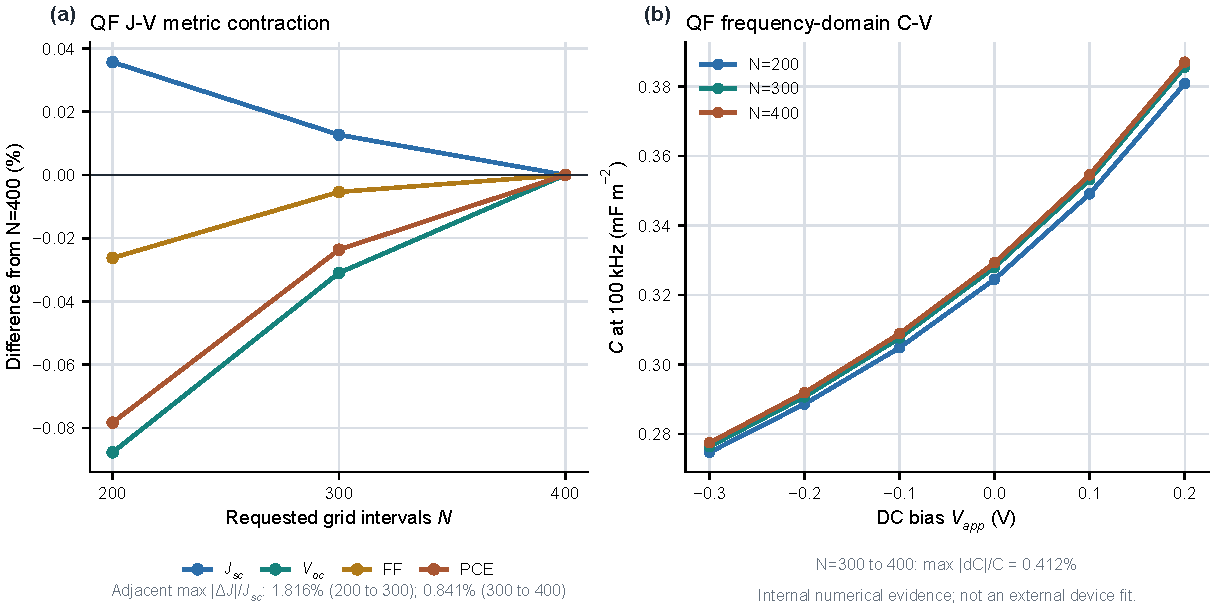
\includegraphics[width=0.98\textwidth,height=\textheight]{figures/csi_qf_convergence.pdf}
\caption{Registered c-Si QF J-V and C-V grid-ladder observations}
\end{figure}

Panel (a) reports each J-V metric relative to the N=400 result and gives
the maximum pointwise current change between adjacent grids. It is a
contraction check against the finest registered grid, not a fitted
order-of-accuracy claim against an exact solution. Panel (b) shows the
stored 100 kHz capacitance values for the same N=200/300/400 ladder.
Both panels are internal numerical evidence for the restricted QF model;
neither is an external c-Si device fit.

\newpage

\begin{figure}
\centering
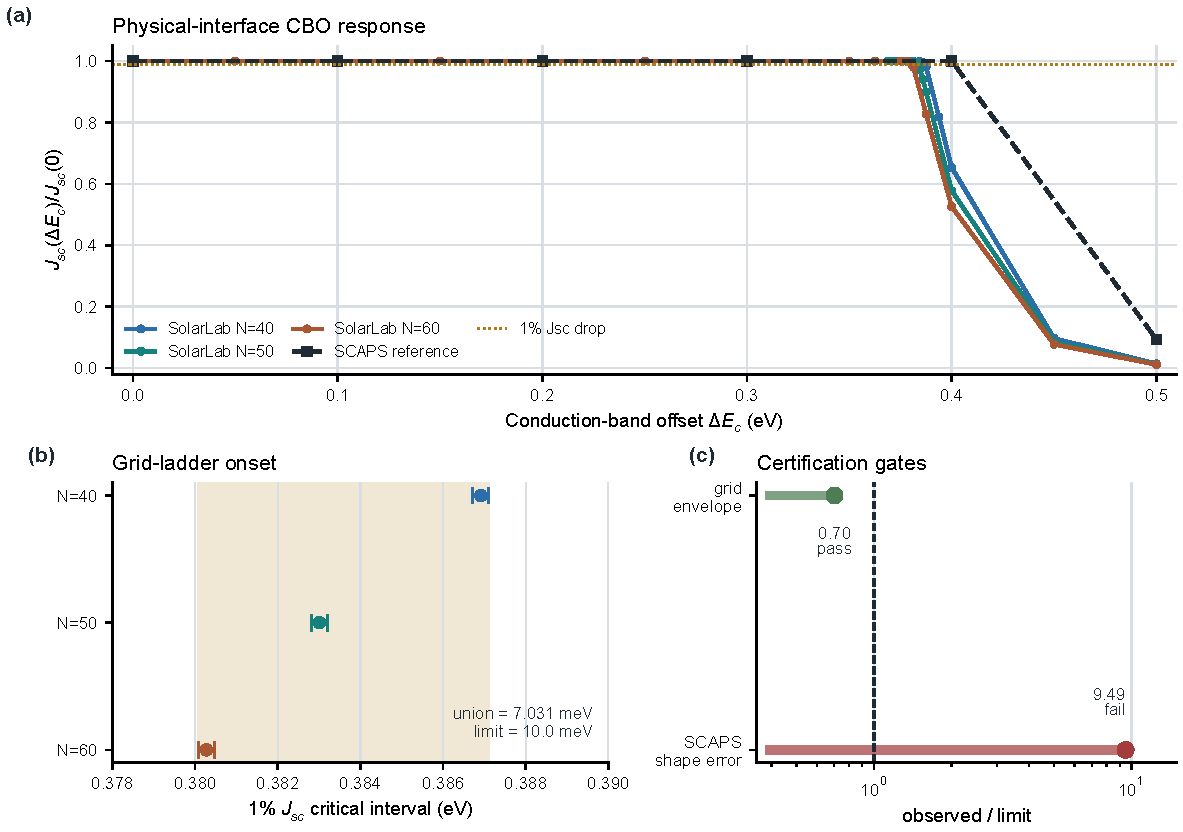
\includegraphics[width=0.98\textwidth,height=\textheight]{figures/cbo_interface_validation.pdf}
\caption{Physical-interface CBO response, grid contraction, and
certification gates}
\end{figure}

The CBO figure reads the complete scan JSON. The SolarLab curves use the
physical zero-thickness interface with \texttt{fermi\_richardson}; the
dashed curve is the registered SCAPS reference. The N=40/50/60
one-percent-\(J_\mathrm{sc}\) intervals form a 7.031 meV union, below
the 10 meV internal numerical limit. The external normalized-shape error
is 0.4744 against a 0.05 limit. The figure therefore shows both parts of
the result: the grid certificate passes, while the top-level external
certificate remains false.

\newpage

\begin{figure}
\centering
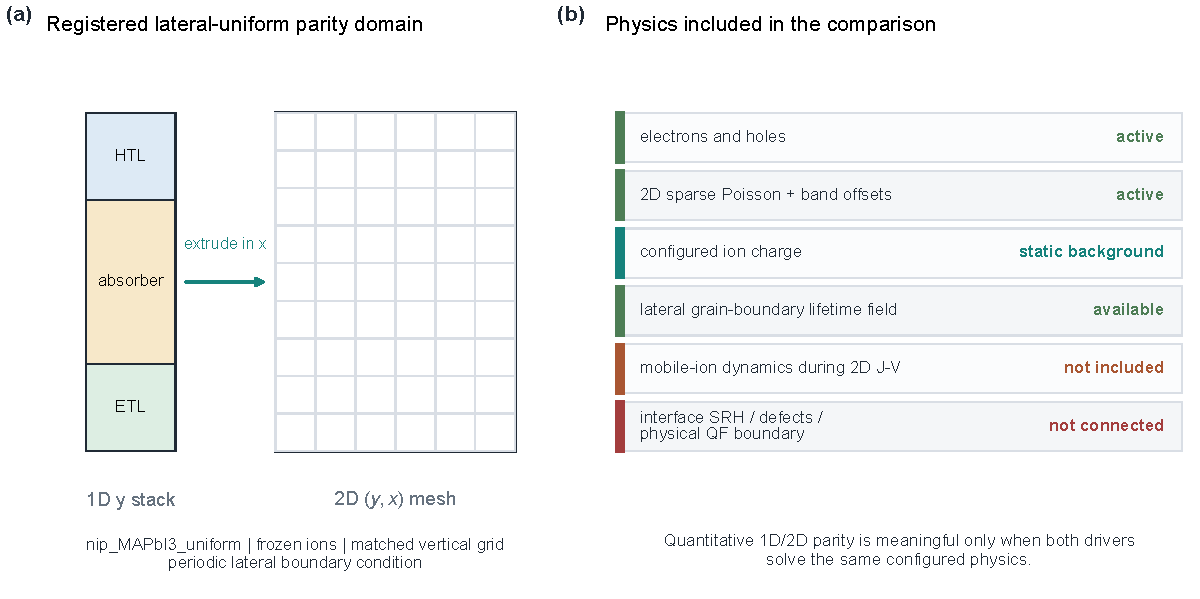
\includegraphics[width=0.98\textwidth,height=\textheight]{figures/twod_scope.pdf}
\caption{Registered 1D/2D parity domain and current model scope}
\end{figure}

The 2D panel is a scope diagram rather than a substitute for stored
result arrays. The registered lateral-uniform comparison freezes ions in
both drivers, matches the vertical grid and uses an interface-free
preset. The 2D solver does not currently consume the 1D interface-SRH,
defect or physical-QF-boundary machinery. Quantitative 1D/2D comparison
on an interface-active stack is therefore outside the validated domain
even when both runs finish.

\hypertarget{other-regression-contracts}{%
\subsection{Other Regression
Contracts}\label{other-regression-contracts}}

The following checks remain useful, but their limits are deterministic
acceptance contracts rather than statistical uncertainties. They are
listed as a table so a tolerance is not mistaken for an error bar.

\begin{longtable}[]{@{}
  >{\raggedright\arraybackslash}p{(\columnwidth - 4\tabcolsep) * \real{0.33}}
  >{\raggedright\arraybackslash}p{(\columnwidth - 4\tabcolsep) * \real{0.33}}
  >{\raggedright\arraybackslash}p{(\columnwidth - 4\tabcolsep) * \real{0.33}}@{}}
\toprule
Contract & Registered value or interval & Interpretation \\
\midrule
\endhead
IonMonger J-V metrics & \(V_\mathrm{oc}=1.1912\,V\),
\(J_\mathrm{sc}=222.59\,A\,m^{-2}\), \(FF=0.7755\), \(PCE=0.2056\);
relative limits 2\%, 3\%, 3\%, 5\% & pinned reverse-scan regression at
\texttt{N\_grid=40}, \texttt{n\_points=20}, \texttt{v\_rate=5.0}; not an
experimental uncertainty \\
TMM \(J_\mathrm{sc}\) & n-i-p 211.02 and p-i-n 216.62 \(A\,m^{-2}\),
each with a \(\pm5\,A\,m^{-2}\) regression tolerance & protects the two
optical baselines from implementation drift; the tolerance is not a
confidence interval \\
Photon-recycling boost & 40--100 mV & literature-informed sanity window
for the recomputed radiative-limit on/off difference; the run value is
not persisted as a manual data series \\
Physical trends & band-gap/current, thickness/voltage, mobility/FF, dark
ideality and Suns-\(V_\mathrm{oc}\) slope & qualitative model checks;
publication plots require the underlying sweep arrays and protocol
metadata \\
2D grain-boundary penalty & 5--100 mV & bounded trend gate on the
registered frozen-ion microstructure case, not a universal MAPbI3
distribution \\
\bottomrule
\end{longtable}

The IonMonger values were re-pinned in July 2026 from 1.1932 V, 231.70
\(A\,m^{-2}\), 0.7774 and 0.2149 when generation was made
photon-conserving. On that configuration the incident photon flux gives
\(q\Phi=224.30\,A\,m^{-2}\), so the superseded \(J_\mathrm{sc}\)
exceeded the available photon budget. Generation is now integrated over
the solver's dual cells, which removes that surplus. The acceptance
percentages were not relaxed.

\hypertarget{validation-traceability-matrix}{%
\section{Validation Traceability
Matrix}\label{validation-traceability-matrix}}

\begingroup\footnotesize\setlength{\tabcolsep}{3.5pt}

\renewcommand{\arraystretch}{1.18}
\begin{longtable}{@{}>{\raggedright\arraybackslash}p{0.24\linewidth}>{\raggedright\arraybackslash}p{0.32\linewidth}>{\raggedright\arraybackslash}p{0.36\linewidth}@{}}
\toprule
Evidence item & Source test or file & What it checks \\
\midrule
\endhead
Current non-slow Python suite & \texttt{pytest -m "not slow"} & broad current-worktree unit/integration coverage for solver, models, backend, experiments, and reproducibility records \\
Frozen P1 slow lane & \path{perovskite-sim/reproducibility/P1_CLOSURE_2026-08-07.md} & expensive regression baselines and the exact acceptance state at P1 closure \\
Current interface/QF target & \path{tests/unit/physics/test_interface_plane_physical_qss.py}, QF/CBO/backend/reproducibility companions & local interface balance, reciprocal transport choices, QF certificates, dispatch, and scan criteria \\
P1 decision registry & \path{perovskite-sim/reproducibility/p1_gaps.yaml} & closed/deferred decisions, reproduction commands, numerical gates, and remaining scientific limits \\
c-Si QF J-V & \path{perovskite-sim/tests/regression/test_csi_quasi_fermi_convergence.py} & 42-point N=200/300/400 grid convergence, photon budget, and per-point physical certificates \\
c-Si QF frequency response & \path{perovskite-sim/tests/regression/test_csi_frequency_domain_impedance.py} & depletion capacitance, storage identity, frequency/step stability, current spread, and linear-solve diagnostics \\
van Nijen c-Si C-V & \path{perovskite-sim/tests/validation/test_csi_vannijen2025_cv.py} & uncalibrated partial external comparison with the 2D/full-area geometry mismatch retained \\
Physical-interface CBO scan & \path{perovskite-sim/outputs/interface-cbo/scan-fermi-edge-qf-grid-40-50-60.json} & internal mesh/statistics certificate and the failed external-shape gate in one result object \\
IonMonger metric envelope & \path{perovskite-sim/tests/integration/test_voc_benchmark.py} & benchmark-scale J-V metrics and hysteresis bounds \\
TMM \(J_\mathrm{sc}\) baselines & \path{perovskite-sim/tests/regression/test_tmm_baseline.py} & optical-stack regression stability \\
Photon-recycling boost & \path{perovskite-sim/tests/regression/test_photon_recycling_voc.py} & radiative-limit voltage boost sanity \\
2D parity & \path{perovskite-sim/tests/regression/test_twod_validation.py} & lateral-uniform 2D consistency with 1D \\
Grain-boundary voltage loss & \path{perovskite-sim/tests/regression/test_twod_microstructure.py} & bounded microstructure-induced voltage penalty \\
Frontend production build & \texttt{npm run build} & TypeScript/Vite production surface \\
Frontend unit tests & \texttt{npm run test:run} & UI result rendering, validation, progress, and workstation state \\
\bottomrule
\end{longtable}
\endgroup

\textsuperscript{a},The frontend checks were run from an isolated
\texttt{/private/tmp} copy using the repository's exact lockfile and the
local npm cache. The OneDrive-resident dependency tree timed out during
direct reads; the local run changes the filesystem location, not the
source or dependency resolution.

The current non-slow Python run reports only \texttt{np.trapz}
deprecation warnings in the compatibility and manufactured-solution
tests. The separate slow command shown in the table is the frozen P1
record unless a newer completed slow pass is stated explicitly; no
unfinished run is counted as evidence.

\hypertarget{scaps-comparison-model-alignment-table}{%
\section{SCAPS Comparison: Model Alignment
Table}\label{scaps-comparison-model-alignment-table}}

Matching input values does not make SCAPS and SolarLab solve the same
problem. They differ in operating mode, contact model, interface
treatment and discretisation, and these choices can change the figures
of merit directly. The table identifies what must be aligned before
comparing a result. Each SolarLab entry was checked against the
implementation; the last column gives the required comparison condition.

\begin{longtable}[]{@{}
  >{\raggedright\arraybackslash}p{(\columnwidth - 6\tabcolsep) * \real{0.25}}
  >{\raggedright\arraybackslash}p{(\columnwidth - 6\tabcolsep) * \real{0.25}}
  >{\raggedright\arraybackslash}p{(\columnwidth - 6\tabcolsep) * \real{0.25}}
  >{\raggedright\arraybackslash}p{(\columnwidth - 6\tabcolsep) * \real{0.25}}@{}}
\toprule
Item & SCAPS & SolarLab & Condition for a valid comparison \\
\midrule
\endhead
Operating mode & Steady state plus linear small signal; no general
transient & Radau/BDF transient, density-based direct steady state,
cancellation-safe QF steady state, and a restricted QF frequency-domain
response & Select the common quantity explicitly. Use
\texttt{steady\_state} for the established ion-frozen comparison, or
\path{quasi_fermi} and \path{quasi_fermi_frequency} where that local
variable set is certified; a transient curve is not definitionally
interchangeable with either \\
Contacts & Metal work function, or a flat-band semiconductor work
function computed per temperature & Explicit metal work functions, or a
Maxwell-Boltzmann semiconductor work-function difference from \(\chi\),
\(E_g\), DOS, doping and temperature; legacy manual override retained
for frozen benchmarks. Ohmic pins and Robin exchange are selected
independently & Use \path{metal_work_function} when the electrode values
are fixed, or \path{semiconductor_work_function} only when the outer
layers represent the same semiconductor reservoirs as SCAPS. Align the
two work functions, contact equilibrium densities and all four surface
velocities separately. A doping sweep moves the semiconductor-derived
potential but must not move an explicitly fixed metal-work-function
difference \\
Temperature & \(N_C,N_V\propto T^{3/2}\);
\(v_\mathrm{th}\propto T^{1/2}\); most other quantities constant &
\(N_C,N_V\propto T^{3/2}\) and \(n_1,p_1\propto n_i(T)/n_i(300)\);
\(\mu\), \(D_\mathrm{ion}\), \(B_\mathrm{rad}\) and \(E_g\) carry
optional laws; per-layer \texttt{v\_th} is imported but has no automatic
\(T^{1/2}\) law & An interface comparison is presently room-temperature
unless the missing thermal-velocity law is supplied and tested
explicitly \\
Interface mesh & Two co-located nodes per interface & Default grid
removes the duplicate point; the opt-in QF boundary carries four
one-sided zero-thickness plane densities eliminated locally & Matching
node count or surface velocity is insufficient. State the topology,
electrical-grid weights/alphas, and the interface support used by each
code \\
Interface transport & Thermionic-emission boundary condition & Default
SG face with an empirical TE cap; alternatively an exclusive physical
boundary with \texttt{fermi\_richardson}, published-SCAPS Boltzmann, or
minimum-thermal-velocity exchange & Compare the actual reciprocal flux
law and statistics. \texttt{scaps\_thermionic} is the closest
equation-level compatibility option, but it remains valid only in its
dilute plane-state regime \\
Interface recombination & Pauwels-Vanhoutte interface states with shared
occupancy & Default surface SRH uses cross-carrier sampling and a
defect-scoped clamp; the exclusive QF boundary uses signed two-sided
capture through one shared occupancy & The defaults are \textbf{not}
equivalent. For the new physical path enable \path{interface_boundary},
report the transport model, and retain the state/DOS and local-residual
certificates; older \path{interface_plane_closure} and
\path{iface_states} results are a separate formulation \\
Tunnelling & WKB, enabled in DC calculations & Static Padovani-Stratton
\(E_{00}\) exponential enhancement & Disable on both sides, or validate
separately. SolarLab's \texttt{interface\_tunneling} is off by default,
so the aligned condition holds without action \\
Grading & Several \(y(x)\), \(P(y)\) and \(P(x)\) laws, including
optical grading & Simplified \(E_g\) and \(\chi\) grading;
\textbf{optics are not graded} & Compare only the common subset. A
graded absorber's absorption edge does not shift spatially in SolarLab,
so \(J_\mathrm{sc}\) reflects the electrical effect alone \\
Mesh & Interface refinement, iterative adaptive & Tanh clustering,
optionally with fixed-budget per-layer weights and alphas & Demonstrate
mesh convergence of the extracted metrics; equal node counts do not
imply equal resolution or allocation \\
Solution method & Gummel with Newton-Raphson sub-steps & Radau/BDF,
density-log Newton, or QF Newton with eliminated Poisson and exact
face-drop coordinates & Compare accepted residuals, continuity and
all-face current conservation, not iteration counts \\
\bottomrule
\end{longtable}

Two differences dominate the comparison used in this chapter. The
optical models are the first. SCAPS integrates a scalar absorption
coefficient with no Fresnel reflection at the transport-layer boundary,
whereas SolarLab runs a coherent transfer-matrix calculation over the
full stack. On the mirrored configuration this accounts for a
\(J_\mathrm{sc}\) of \(218.2\,\mathrm{A\,m^{-2}}\) against the SCAPS
\(262.8\,\mathrm{A\,m^{-2}}\), a \(-17\,\%\) difference. This value uses
the photon-conserving generation quadrature; point-sampling the
front-weighted generation profile would over-count absorbed photons and
understate the model difference. Resolving it requires a SCAPS-matched
optical calculation; changing an electrical parameter does not address
the source of the discrepancy.

The second difference is the set of default choices. Contacts, interface
recombination, transport statistics and thermionic normalisation all
have alternatives that are off by default. Turning one on does not by
itself validate the model. The physical interface boundary now solves
transport and shared-occupancy SRH conservatively, but the current CBO
campaign passes only the internal grid tests and still fails the
declared SCAPS shape test. Reports must state the selected option and
whether the agreement is internal numerical or external.

\hypertarget{limitations-and-best-practices}{%
\chapter{Limitations And Best
Practices}\label{limitations-and-best-practices}}

\hypertarget{model-assumptions}{%
\section{Model Assumptions}\label{model-assumptions}}

SolarLab is a numerical research simulator. Predictive accuracy for a
material stack requires physically justified inputs and a validation
envelope that covers the intended regime.

\hypertarget{known-formulation-limitations}{%
\section{Known Formulation
Limitations}\label{known-formulation-limitations}}

The following model-formulation limitations apply, each flagged at its
point of use in Chapter \ref{governing-equations}:

\begin{itemize}
\tightlist
\item
  the default thermionic-emission bound is an empirical density-weighted
  cap, not the dimensionally normalized Richardson-Dushman current. The
  physical emission-velocity form is available through
  \path{te_physical_norm} and the previously identified sign,
  barrier-input and DOS-consistency defects are corrected. It remains
  opt-in because strongly binding faces still expose conditioning limits
  in some weak-contact, cold-start and deep-injection regimes. Users who
  enable it should verify equilibrium zero current, bias continuation,
  grid convergence and the intended operating window;
\item
  the ionic steric flux now defaults to the diffusion-only modified-PNP
  form (\path{ion_steric_diffusion_only}), so the crowding chemical
  potential modifies diffusion without artificially amplifying field
  drift. The \path{legacy} tier retains the superseded whole-flux
  multiplier for frozen IonMonger comparisons. The current model is
  still a single-site lattice gas: it includes site exclusion but not
  ion-ion correlations, and its near-saturation behaviour is covered by
  flux-level tests rather than a registered device preset;
\item
  the interface-SRH non-negativity clamp applies only at declared-defect
  interfaces. The older cross-carrier approximation can otherwise use a
  cross-side majority-density product as its detailed-balance reference,
  which is not a local mass-action reference. Defect-free interfaces
  retain signed generation. Reverse-bias or dark-current studies that
  depend on the sign of interface generation should use the physically
  referenced interface-plane closure and report that choice;
\item
  the exclusive QF interface boundary removes the support and
  detailed-balance ambiguities of that default cross-carrier
  approximation: ordinary SG transport is removed at the boundary, one
  shared signed occupancy closes capture and emission, and the four
  positive plane states are eliminated under an explicit residual
  certificate. Current evidence is internal: the registered N=40/50/60
  CBO scan passes its numerical grid and local-residual gates, but its
  finest normalized SCAPS \(J_\mathrm{sc}\) error is 0.4744 against a
  0.05 external-shape gate. The path is a grid-certified development
  model; these data do not establish an external CBO threshold;
\item
  the photon-recycling redistribution is spatially uniform, with no
  spatial or spectral reabsorption kernel;
\item
  the Scharfetter-Gummel positivity property is a property of the
  \emph{spatial} semi-discretization. The transient advances \((n,p,P)\)
  with a general-purpose implicit integrator and applies no clipping or
  projection, so non-negativity is not guaranteed at every internal
  stage or accepted step. The direct steady-state driver does enforce
  it, by solving in logarithmic unknowns;
\item
  the slow-ion operator splitting freezes the carriers over the
  macro-step and re-solves Poisson inside the ion RHS. That makes the
  field consistent with the instantaneous charge density but does not
  hold the carriers quasi-stationary against the evolving ionic field,
  so it is a first-order splitting whose error grows with the macro-step
  and with the ion-induced band bending;
\item
  per-layer interface thermal velocities can now be supplied directly
  and are imported by the SCAPS loader, but neither they nor the
  density-of-states prefactor of the per-side interface-defect trap
  levels carry an automatic temperature law. Interface formulations
  using them are therefore room-temperature models unless the missing
  dependence is supplied and validated explicitly.
\end{itemize}

High-occupancy tests showed that the old whole-flux steric multiplier
produced the wrong trend, so the modified-PNP form is now the default.
The normalized thermionic cap remains opt-in because convergence has not
been demonstrated over a sufficiently broad set of strongly binding
cases. These decisions apply only to the tested regimes; they do not
rank the two models in every device class.

\hypertarget{data-and-optical-limits}{%
\section{Data And Optical Limits}\label{data-and-optical-limits}}

TMM, EQE, and EL depend on tabulated \(n,k\) data. \texttt{load\_nk}
does not silently extrapolate outside the source wavelength range.
Placeholder optical constants support workflow testing, but they do not
support material-specific publication claims.

\hypertarget{numerical-limits}{%
\section{Numerical Limits}\label{numerical-limits}}

If a J-V sweep does not bracket \(V_\mathrm{oc}\), first distinguish a
scan that stopped above the current-resolution floor from a bracket
rejected by the thermodynamic ceiling. Increase \texttt{V\_max} only in
the first case, and refine the voltage grid near the expected bracket
when its sampling uncertainty matters. Sentinel zero FF or PCE should
not be interpreted as physical failure until \texttt{voc\_bracketed} and
the associated limits have been checked.

Mott-Schottky fits can be unreliable for fully depleted thin absorbers.

Thick CIGS and crystalline silicon absorbers can be slow in transient
mode.

The shipped crystalline-silicon homojunction requires the
cancellation-safe QF driver for production J-V calculations. On the same
N=200, \(V=0\) one-sun state, the QF residual is \(5.82\times10^{-13}\)
while the collapsed density-SG residual is 33.08. The general
transient/algebraic state remains deferred until a compensated dynamic
mass-matrix or equivalent representation independently passes the
registered voltage and grid gates. A QF result must not be cited as a
converged transient result.

The QF frequency-domain path certifies the restricted local c-Si C-V
model; it does not repair the default time-domain path, whose endpoint
conduction and interval-averaged displacement sampling returned the
whole-wafer geometric capacitance in the audited case. Mobile-ion
impedance still requires the time-domain model, together with an
explicit settling and amplitude study.

\hypertarget{d-limits}{%
\section{2D Limits}\label{d-limits}}

The 2D solver freezes ions. It is suitable for lateral parity and
microstructure studies under that approximation, but not for full
dynamic ion migration in two dimensions.

\hypertarget{reporting-checklist}{%
\section{Reporting Checklist}\label{reporting-checklist}}

A reproducible SolarLab study should report:

\begin{itemize}
\tightlist
\item
  commit hash;
\item
  device YAML or full parameter table;
\item
  physics tier;
\item
  grid settings;
\item
  solver driver, variable set, and tolerances;
\item
  interface-boundary flag, transport law, and QF coordinate system when
  used;
\item
  optical data source;
\item
  validation command results;
\item
  evidence label (\texttt{certified}, \texttt{partial},
  \texttt{load\_only}, \texttt{demo}, or \texttt{unvalidated}) and the
  acceptance criteria it refers to;
\item
  whether \(V_\mathrm{oc}\) was bracketed;
\item
  known limitations relevant to the chosen experiment.
\end{itemize}

\hypertarget{before-publication}{%
\section{Before Publication}\label{before-publication}}

Before publishing a SolarLab figure, verify all of the following:

\begin{itemize}
\tightlist
\item
  the device stack and all changed parameters are reported;
\item
  optical constants and material parameters have provenance;
\item
  the chosen physics tier is justified;
\item
  the grid and solver settings are sufficient for the conclusion;
\item
  validation gates relevant to the claimed regime have passed;
\item
  any internal numerical certificate is kept separate from external
  physical agreement;
\item
  limitations such as frozen 2D ions, placeholder optical data, or
  screening smoke settings are stated explicitly.
\end{itemize}

If any item is missing, the result may still be useful for debugging or
hypothesis screening, but it should not be described as a calibrated
material-specific prediction.

\hypertarget{solarscale-screening-bridge}{%
\chapter{SolarScale Screening
Bridge}\label{solarscale-screening-bridge}}

SolarLab can consume readiness-gated material records from SolarScale.
This is a workflow layer, not the core solver.

Safe mappings include:

\begin{itemize}
\tightlist
\item
  dielectric constant to \texttt{eps\_r};
\item
  electron and hole mobility to \texttt{mu\_n} and \texttt{mu\_p} after
  unit conversion;
\item
  ion diffusion to \texttt{D\_ion};
\item
  ion activation energy to \texttt{E\_a\_ion};
\item
  electron affinity (\texttt{electron\_affinity\_ev}) to the absorber
  \texttt{chi} --- with the caution that this parameter directly sets
  the band alignment at both heterojunctions, so its provenance and
  uncertainty must accompany any screening result that depends on it.
\end{itemize}

Device-only unknowns should be swept rather than guessed:

\begin{itemize}
\tightlist
\item
  absorber thickness;
\item
  SRH lifetime;
\item
  trap density;
\item
  interface recombination velocity;
\item
  contact band alignment.
\end{itemize}

Smoke J-V results in screening workflows validate the process. They are
not publication-grade device predictions unless production settings,
provenance, and validation are also supplied.

\hypertarget{references}{%
\chapter{References}\label{references}}

\begin{enumerate}
\def\labelenumi{\arabic{enumi}.}
\tightlist
\item
  D. L. Scharfetter and H. K. Gummel, ``Large-signal analysis of a
  silicon Read diode oscillator,'' \emph{IEEE Transactions on Electron
  Devices} \textbf{16}, 64--77 (1969). doi:10.1109/T-ED.1969.16566.
\item
  W. Shockley and W. T. Read, ``Statistics of the recombinations of
  holes and electrons,'' \emph{Physical Review} \textbf{87}, 835--842
  (1952). doi:10.1103/PhysRev.87.835.
\item
  R. N. Hall, ``Electron-hole recombination in germanium,''
  \emph{Physical Review} \textbf{87}, 387 (1952).
  doi:10.1103/PhysRev.87.387.
\item
  N. E. Courtier, J. M. Cave, J. M. Foster, A. B. Walker, and G.
  Richardson, ``IonMonger: a free and fast planar perovskite solar cell
  simulator with coupled ion vacancy and charge carrier dynamics,''
  \emph{Journal of Computational Electronics} \textbf{18}, 1435--1449
  (2019). doi:10.1007/s10825-019-01396-2.
\item
  P. Calado, I. Gelmetti, B. Hilton, M. Azzouzi, J. Nelson, and P. R. F.
  Barnes, ``Driftfusion: an open source code for simulating ordered
  semiconductor devices with mixed ionic-electronic conducting materials
  in one dimension,'' \emph{Journal of Computational Electronics}
  \textbf{21}, 960--991 (2022). doi:10.1007/s10825-021-01827-z.
\item
  M. Burgelman, P. Nollet, and S. Degrave, ``Modelling polycrystalline
  semiconductor solar cells,'' \emph{Thin Solid Films}
  \textbf{361--362}, 527--532 (2000). doi:10.1016/S0040-6090(99)00825-1.
\item
  U. Rau, ``Reciprocity relation between photovoltaic quantum efficiency
  and electroluminescent emission of solar cells,'' \emph{Physical
  Review B} \textbf{76}, 085303 (2007). doi:10.1103/PhysRevB.76.085303.
\item
  L. A. A. Pettersson, L. S. Roman, and O. Inganäs, ``Modeling
  photocurrent action spectra of photovoltaic devices based on organic
  thin films,'' \emph{Journal of Applied Physics} \textbf{86}, 487--496
  (1999). doi:10.1063/1.370757.
\item
  E. Yablonovitch, ``Statistical ray optics,'' \emph{Journal of the
  Optical Society of America} \textbf{72}, 899--907 (1982).
  doi:10.1364/JOSA.72.000899.
\item
  D. M. Caughey and R. E. Thomas, ``Carrier mobilities in silicon
  empirically related to doping and field,'' \emph{Proceedings of the
  IEEE} \textbf{55}, 2192--2193 (1967). doi:10.1109/PROC.1967.6123.
\item
  J. Frenkel, ``On pre-breakdown phenomena in insulators and electronic
  semiconductors,'' \emph{Physical Review} \textbf{54}, 647--648 (1938).
  doi:10.1103/PhysRev.54.647.
\item
  M. A. Green, ``Solar cell fill factors: General graph and empirical
  expressions,'' \emph{Solid-State Electronics} \textbf{24}, 788--789
  (1981). doi:10.1016/0038-1101(81)90062-9.
\item
  J. Nelson, \emph{The Physics of Solar Cells} (Imperial College Press,
  London, 2003).
\item
  P. Würfel, \emph{Physics of Solar Cells: From Principles to New
  Concepts} (Wiley-VCH, Weinheim, 2005).
\item
  H. J. Snaith, ``Perovskites: The emergence of a new era for low-cost,
  high-efficiency solar cells,'' \emph{Journal of Physical Chemistry
  Letters} \textbf{4}, 3623--3630 (2013). doi:10.1021/jz4020162.
\item
  L. M. Pazos-Outón et al., ``Photon recycling in lead iodide perovskite
  solar cells,'' \emph{Science} \textbf{351}, 1430--1433 (2016).
  doi:10.1126/science.aaf1168.
\item
  S. Selberherr, \emph{Analysis and Simulation of Semiconductor Devices}
  (Springer, Vienna, 1984).
\item
  E. Hairer and G. Wanner, \emph{Solving Ordinary Differential Equations
  II: Stiff and Differential-Algebraic Problems}, 2nd ed.~(Springer,
  Berlin, 1996).
\item
  G. F. Burkhard, E. T. Hoke, and M. D. McGehee, ``Accounting for
  interference, scattering, and electrode absorption to make accurate
  internal quantum efficiency measurements in organic and other thin
  solar cells,'' \emph{Advanced Materials} \textbf{22}, 3293--3297
  (2010). doi:10.1002/adma.201000883.
\item
  F. A. Padovani and R. Stratton, ``Field and thermionic-field emission
  in Schottky barriers,'' \emph{Solid-State Electronics} \textbf{9},
  695--707 (1966). doi:10.1016/0038-1101(66)90097-9.
\item
  Y. P. Varshni, ``Temperature dependence of the energy gap in
  semiconductors,'' \emph{Physica} \textbf{34}, 149--154 (1967).
  doi:10.1016/0031-8914(67)90062-6.
\item
  M. S. Kilic, M. Z. Bazant, and A. Ajdari, ``Steric effects in the
  dynamics of electrolytes at large applied voltages. II. Modified
  Poisson-Nernst-Planck equations,'' \emph{Physical Review E}
  \textbf{75}, 021503 (2007). doi:10.1103/PhysRevE.75.021503.
\item
  H. Pauwels and G. Vanhoutte, ``The influence of interface state and
  energy barriers on the efficiency of heterojunction solar cells,''
  \emph{Journal of Physics D: Applied Physics} \textbf{11}, 649--667
  (1978). doi:10.1088/0022-3727/11/5/009.
\item
  M. Burgelman and J. Marlein, ``Analysis of graded band gap solar cells
  with SCAPS,'' \emph{Proceedings of the 23rd European Photovoltaic
  Solar Energy Conference}, 2151--2155 (2008).
\item
  Y. F. Chang, ``The capacitance of p-n junctions,'' \emph{Solid-State
  Electronics} \textbf{10}, 281--287 (1967).
  doi:10.1016/0038-1101(67)90014-7.
\item
  M. Hufschmidt et al., ``The influence of edge effects on the
  determination of the doping profile of silicon pad diodes,''
  arXiv:1605.00778v1 (2016).
\item
  J. Verschraegen and M. Burgelman, ``Numerical modeling of intra-band
  tunneling for heterojunction solar cells in SCAPS,'' \emph{Thin Solid
  Films} \textbf{515}, 6276--6279 (2007).
\item
  D. A. van Nijen et al., ``The nature of silicon PN junction impedance
  at high frequency,'' \emph{Solar Energy Materials and Solar Cells}
  \textbf{282}, 113383 (2025). doi:10.1016/j.solmat.2024.113383.
\end{enumerate}

\hypertarget{appendix-a-documentation-sources}{%
\chapter{Appendix A: Documentation
Sources}\label{appendix-a-documentation-sources}}

This manual describes the current implementation, the reason for unusual
defaults, known limitations and the evidence behind the stated
conclusions. It does not keep a development diary. Include a failed
approach only when it changed the physical interpretation or still
determines a default or operating limit. Detailed iteration history
remains in \texttt{perovskite-sim/CLAUDE.md}, the reproducibility
records and version-control history.

The manual was drafted from:

\begin{itemize}
\item
  \texttt{docs/solarlab\_manual\_source\_dossier.md} (removed
  2026-07-29; in git history at \texttt{db700fe})
\item
  \texttt{docs/manual/valEvidence260723.md} (historical 2026-07-23 pass)
\item
  \texttt{docs/manual/valEvidence260519.md} (superseded 2026-05-19 pass)
\item
  \texttt{perovskite-sim/reproducibility/P1\_CLOSURE\_2026-08-07.md}
\item
  \texttt{perovskite-sim/reproducibility/p1\_gaps.yaml}
\item
  \texttt{perovskite-sim/docs/physical-interface-cbo-scan.md}
\item
  \path{perovskite-sim/outputs/interface-cbo/scan-fermi-edge-qf-grid-40-50-60.json}
\item
  \texttt{perovskite-sim/CLAUDE.md}
\item
  \texttt{README.md}
\item
  \texttt{perovskite-sim/README.md}
\item
  \texttt{perovskite-sim/backend/README.md}
\item
  \texttt{perovskite-sim/perovskite\_sim/models/}
\item
  \texttt{perovskite-sim/perovskite\_sim/physics/}
\item
  \texttt{perovskite-sim/perovskite\_sim/solver/}
\item
  \texttt{perovskite-sim/perovskite\_sim/experiments/}
\item
  \texttt{perovskite-sim/perovskite\_sim/experiments/quasi\_fermi\_steady\_state.py}
\item
  \texttt{perovskite-sim/perovskite\_sim/experiments/quasi\_fermi\_impedance.py}
\item
  \texttt{perovskite-sim/perovskite\_sim/physics/interface\_plane.py}
\item
  \texttt{perovskite-sim/perovskite\_sim/twod/}
\item
  \texttt{perovskite-sim/backend/main.py}
\item
  \texttt{perovskite-sim/frontend/src/types.ts}
\end{itemize}

This PDF is intended to be defensible as a project manual. For a journal
supplement, add parameter provenance for every material value and verify
the full bibliography format against the target journal style.

\hypertarget{appendix-b-figure-sources}{%
\chapter{Appendix B: Figure Sources}\label{appendix-b-figure-sources}}

\begingroup\footnotesize\setlength{\tabcolsep}{3.5pt}

\renewcommand{\arraystretch}{1.18}
\begin{longtable}{@{}>{\raggedright\arraybackslash}p{0.24\linewidth}>{\raggedright\arraybackslash}p{0.32\linewidth}>{\raggedright\arraybackslash}p{0.36\linewidth}@{}}
\toprule
Figure & Source & Reproducibility note \\
\midrule
\endhead
Architecture and data flow & \path{docs/manual/generate_manual_figures.py} & Implementation diagram checked against the shared schema, material-cache and explicit driver dispatch paths. \\
Device and contact boundary & \path{perovskite-sim/perovskite_sim/models/device.py}, \path{perovskite-sim/perovskite_sim/solver/mol.py} & Shows YAML layer order, signed contact-potential sources and the independent carrier-contact law. \\
Band and interface conventions & \path{perovskite-sim/perovskite_sim/physics/continuity.py}, \path{perovskite-sim/perovskite_sim/physics/interface_plane.py} & Schematic energy convention; no material-specific solved band profile is implied. \\
Solver topology & \path{perovskite-sim/perovskite_sim/experiments/} and \path{perovskite-sim/perovskite_sim/twod/} & Separates transient, direct steady-state, QF DC, QF frequency and 2D variable sets. \\
c-Si QF convergence & \path{perovskite-sim/reproducibility/config_benchmark_matrix.yaml} & Reads registered N=200/300/400 J-V metrics, adjacent-curve changes and 100 kHz C-V arrays. \\
Physical-interface CBO & \path{perovskite-sim/outputs/interface-cbo/scan-fermi-edge-qf-grid-40-50-60.json} & Reads the full traces, critical intervals and separate internal/external certification gates. \\
2D model scope & \path{perovskite-sim/perovskite_sim/twod/solver_2d.py}, \path{perovskite-sim/tests/regression/test_twod_validation.py} & Identifies the registered parity domain and the interface-physics boundary without inventing unrecorded observations. \\
\bottomrule
\end{longtable}
\endgroup

\hypertarget{appendix-c-glossary}{%
\chapter{Appendix C: Glossary}\label{appendix-c-glossary}}

\begin{longtable}[]{@{}
  >{\raggedright\arraybackslash}p{(\columnwidth - 2\tabcolsep) * \real{0.50}}
  >{\raggedright\arraybackslash}p{(\columnwidth - 2\tabcolsep) * \real{0.50}}@{}}
\toprule
Term & Meaning \\
\midrule
\endhead
AM1.5G & Standard terrestrial solar spectrum used for photovoltaic
testing. \\
Beer-Lambert & Scalar absorption law using an absorption coefficient
\(\alpha\). \\
Bernoulli function & \(B(\xi)=\xi/(e^{\xi}-1)\); the weighting function
of the Scharfetter-Gummel flux. \\
Detailed balance & Requirement that every generation/recombination
channel vanishes exactly at thermodynamic equilibrium. \\
Displacement current & Capacitive current
\(\varepsilon_0\varepsilon_r\,\partial E/\partial t\) included in the
terminal current. \\
Drift-diffusion & Continuum transport model combining diffusion from
concentration gradients and drift from electric fields. \\
FF & Fill factor, the ratio between maximum power and
\(V_\mathrm{oc}J_\mathrm{sc}\). \\
Hysteresis & Difference between forward and reverse J-V scans caused by
state memory, often ionic in perovskites. \\
Quasi-Fermi potential & Electrochemical carrier potential whose spatial
drop drives electron or hole current; SolarLab stores reference and
increment separately in cancellation-sensitive solves. \\
Ideality factor & Slope parameter \(n_\mathrm{id}\) of the dark diode
characteristic. \\
Method of lines & Numerical method that discretizes space first and
integrates the resulting ODE system in time. \\
PCE & Power-conversion efficiency. \\
Photon recycling & Reabsorption of internally emitted photons, reducing
the net radiative loss. \\
Quasi-Fermi level & Electrochemical potential of one carrier population
out of equilibrium; flat quasi-Fermi levels mean zero current. \\
Radau IIA & L-stable fully implicit Runge-Kutta method used for the
stiff time integration. \\
Richardson constant & Prefactor \(A^{*}\) of the thermionic-emission
flux across a band offset. \\
SG flux & Scharfetter-Gummel flux discretization, used for stable
drift-dominated carrier transport. \\
SRH & Shockley-Read-Hall trap-assisted recombination. \\
Steric site density & Finite-site scale \(P_\mathrm{lim}\) entering the
mobile-ion crowding chemical potential; it is not a hard transient-state
bound. \\
Thermionic emission & Interface-limited carrier transport over a
heterojunction band offset. \\
TMM & Transfer-matrix method for wavelength-resolved multilayer
optics. \\
\(J_\mathrm{sc}\) & Short-circuit current density. \\
\(V_\mathrm{oc}\) & Open-circuit voltage. \\
\bottomrule
\end{longtable}

\end{document}
